\PassOptionsToPackage{unicode=true}{hyperref} % options for packages loaded elsewhere
\PassOptionsToPackage{hyphens}{url}
\PassOptionsToPackage{dvipsnames,svgnames*,x11names*}{xcolor}
%
\documentclass[11pt,french,landscape]{article}
\usepackage{lmodern}
\usepackage{amssymb,amsmath}
\usepackage{ifxetex,ifluatex}
\usepackage{fixltx2e} % provides \textsubscript
\ifnum 0\ifxetex 1\fi\ifluatex 1\fi=0 % if pdftex
  \usepackage[T1]{fontenc}
  \usepackage[utf8]{inputenc}
  \usepackage{textcomp} % provides euro and other symbols
\else % if luatex or xelatex
  \usepackage{unicode-math}
  \defaultfontfeatures{Ligatures=TeX,Scale=MatchLowercase}
\fi
% use upquote if available, for straight quotes in verbatim environments
\IfFileExists{upquote.sty}{\usepackage{upquote}}{}
% use microtype if available
\IfFileExists{microtype.sty}{%
\usepackage[]{microtype}
\UseMicrotypeSet[protrusion]{basicmath} % disable protrusion for tt fonts
}{}
\IfFileExists{parskip.sty}{%
\usepackage{parskip}
}{% else
\setlength{\parindent}{0pt}
\setlength{\parskip}{6pt plus 2pt minus 1pt}
}
\usepackage{xcolor}
\usepackage{hyperref}
\hypersetup{
            pdfauthor={Julien Gossa gossa@unistra.fr},
            colorlinks=true,
            linkcolor=blue,
            filecolor=Maroon,
            citecolor=Blue,
            urlcolor=blue,
            breaklinks=true}
\urlstyle{same}  % don't use monospace font for urls
\usepackage[margin=1.5cm]{geometry}
\usepackage{graphicx,grffile}
\makeatletter
\def\maxwidth{\ifdim\Gin@nat@width>\linewidth\linewidth\else\Gin@nat@width\fi}
\def\maxheight{\ifdim\Gin@nat@height>\textheight\textheight\else\Gin@nat@height\fi}
\makeatother
% Scale images if necessary, so that they will not overflow the page
% margins by default, and it is still possible to overwrite the defaults
% using explicit options in \includegraphics[width, height, ...]{}
\setkeys{Gin}{width=\maxwidth,height=\maxheight,keepaspectratio}
\setlength{\emergencystretch}{3em}  % prevent overfull lines
\providecommand{\tightlist}{%
  \setlength{\itemsep}{0pt}\setlength{\parskip}{0pt}}
\setcounter{secnumdepth}{5}
% Redefines (sub)paragraphs to behave more like sections
\ifx\paragraph\undefined\else
\let\oldparagraph\paragraph
\renewcommand{\paragraph}[1]{\oldparagraph{#1}\mbox{}}
\fi
\ifx\subparagraph\undefined\else
\let\oldsubparagraph\subparagraph
\renewcommand{\subparagraph}[1]{\oldsubparagraph{#1}\mbox{}}
\fi

% set default figure placement to htbp
\makeatletter
\def\fps@figure{htbp}
\makeatother

%\usepackage[utf8x]{inputenc}
\usepackage{eurosym}
%\usepackage{draftwatermark}
\usepackage[default]{raleway}
\usepackage[strict]{changepage}
\usepackage{multicol}
\usepackage{calc}
\usepackage{tikz}
\usetikzlibrary{
  calc,
  positioning
}

\def\arraystretch{1.5}

% \usepackage{fancyhdr}
% \makeatletter
% \renewcommand{\@chapapp}{Partie}
% \makeatother
\usepackage{booktabs}
\usepackage{longtable}
\usepackage{array}
\usepackage{multirow}
\usepackage{wrapfig}
\usepackage{float}
\usepackage{colortbl}
\usepackage{pdflscape}
\usepackage{tabu}
\usepackage{threeparttable}
\usepackage{threeparttablex}
\usepackage[normalem]{ulem}
\usepackage{makecell}
\usepackage{xcolor}
\ifnum 0\ifxetex 1\fi\ifluatex 1\fi=0 % if pdftex
  \usepackage[shorthands=off,main=french]{babel}
\else
  % load polyglossia as late as possible as it *could* call bidi if RTL lang (e.g. Hebrew or Arabic)
  \usepackage{polyglossia}
  \setmainlanguage[]{french}
\fi

\author{Julien Gossa\\
\href{mailto:gossa@unistra.fr}{\nolinkurl{gossa@unistra.fr}}}
\date{09/01/2020}

\begin{document}


\newcommand\titre{Tableaux de bord \\ des établissements de \\ l'Enseignement Supérieur \\ et de la Recherche}
\newcommand\auteur{Julien Gossa}
\newcommand\rentree{Edition 2018-2019}
\newcommand\ladate{Mai 2020}
\newcommand\reportid{tdbesr-2018-v1.0}

\definecolor{royalblue(traditional)}{rgb}{0.0, 0.14, 0.4}
\definecolor{royalblue(web)}{rgb}{0.25, 0.41, 0.88}

\newcommand\titleY{0cm}
\newcommand\titleS{3}
\newcommand\titleBoxW{19cm}
\newcommand\titleBoxH{11cm}
\newcommand\titleBoxR{7}


\begin{titlepage}

\begin{tikzpicture}[overlay,remember picture]

  \coordinate (logo) at (current page.north west);
  \coordinate (title) at ($(current page.center) + (0,\titleY)$);
  \coordinate (author) at (current page.south east);

\node (nlogo) [inner sep=20pt, anchor=north west] at (logo)
  {
\includegraphics[width=8cm]{files/logo_cpesr_sackersgothic}};

\node (bandeau) at (title) 
  [draw, minimum width=\titleBoxW, minimum height=\titleBoxH, rotate=\titleBoxR, color=royalblue(web), fill=royalblue(web)] {};

\node (ntitle) at (title) 
  [inner sep=0pt, anchor=center, align=center, font=\bfseries, scale=\titleS, align=center, color=white]  
  {\titre};

\node (nrentree) at ($(bandeau.south west)!0.95!(bandeau.south east)$)
  [inner sep=10pt, anchor=south east, rotate=\titleBoxR, font=\Huge, color=white]
  {\rentree};

\node (num) at ($(bandeau.south west)!0.94!(bandeau.south east)$)
  [inner sep=5pt, anchor=north east, rotate=\titleBoxR, font=\large]
  {\reportid};

\node (nauteur) at (author) 
  [inner sep=50pt, anchor=south east, align=center, font=\huge, align=left, color =black]
  {\textbf{\ladate} \\ \auteur};

  
\end{tikzpicture}

\end{titlepage}



\newlength{\graphesX}
\setlength{\graphesX}{30pt}
\newlength{\graphesY}
\setlength{\graphesY}{-7cm}
\newlength{\graphesW}
\setlength{\graphesW}{0.52\textwidth}

\newcommand\maketdb[4]{
  \begin{tikzpicture}[overlay,remember picture]
    \node (ancetres) [inner sep=0pt, anchor=north west, xshift=\graphesX, yshift=\graphesY] at (current page.north west)
      {\includegraphics[width=0.5\graphesW]{#1}};
    \node (associations) [inner sep=0pt, anchor=west] at (ancetres.east)
      {\includegraphics[width=0.5\graphesW]{#2}};
    \node (composantes) [inner sep=0pt, anchor=north west,yshift=-30pt] at (ancetres.south west)
      {\includegraphics[width=\graphesW]{#3}};
      
    \node (kpi) [inner sep=30pt, anchor=north east] at (current page.north east)
      {\includegraphics[width=\graphesW]{#4}};

    \node (ancetres-tit) [inner sep=0pt, anchor=south] at (ancetres.north) {\bf Filiation};
    \node (associations-tit) [inner sep=0pt, anchor=south] at (associations.north) {\bf Association};
    \node (composantes-tit) [inner sep=0pt, anchor=south] at (composantes.north) {\bf Composition};

  \end{tikzpicture}
}

\hypertarget{avant-propos}{%
\section*{Avant-propos}\label{avant-propos}}
\addcontentsline{toc}{section}{Avant-propos}

Apparaissant dès le XIIIe siècle, les universités sont des organisations
à la durée de vie particulièrement longue. Leur évolution est permanente
et se fait sous différentes tensions, notamment sociales et politiques,
culturelles et cultuelles, ou encore démographiques et géographique, qui
touchent à la profession même des universitaires. Depuis le tournant du
XXIe siècle, un mouvement de profonde transformation de l'Enseignement
supérieur et rechercher (ESR) est engagé :

\begin{itemize}
\tightlist
\item
  La Loi liberté et responsabilités des universités (LRU) amorce en 2007
  un mouvement dit d'«~autonomie des universités~», adossé notamment aux
  responsabilités et compétences élargies (RCE), qui transfèrent la
  masse salariale du ministère aux établissements. Les universités sont
  ainsi invitées à développer leur propre politique d'emploi.
\item
  Onze universités sont sélectionnées pour l'Initiative d'excellence
  (IDEX) sur un projet de gouvernance différenciant dans le cadre du
  Plan d'investissement d'avenir (PIA).
\item
  Un nombre exceptionnel de fusions et regroupements est organisé,
  d'abord autour des Pôles de recherche et d'enseignement supérieur
  (PRES) puis des Communautés d'universités et d'établissements (COMUE).
\end{itemize}

Ces transformations conduisent à des évolutions structurelles locales
qui favorisent les divergences entre les établissements de l'ESR. Ces
divergences se retrouvent à tous les niveaux de détail, par exemple dans
le pyramidage LMD de l'effectif étudiant, et le pyramidage PR-MCF-2d
degré de l'effectif enseignant. Il existe donc un besoin nouveau et
croissant d'outils de suivi et d'analyse des caractéristiques et
politiques des établissements de l'ESR.

Ce document propose donc une sélection d'indicateurs primaires
suffisament peu nombreux et complexes pour être rapidement utilisables,
puis une construction d'indicateurs clés permettant de leur donner du
sens.

\vspace*{\fill}

\begin{center}
\includegraphics[width=200px,height=0.3\textheight]{files/589px-Knowledge-Reid-Highsmith} \end{center}

\newpage
\begin{multicols}{2}
\tableofcontents
\newpage
\part{Présentation des données}

Il existe trois sources principales d'informations sur les
établissements de l'ESR français :

\begin{itemize}
\tightlist
\item
  \href{https://www.data.gouv.fr/fr/}{data.gouv.fr} : le portail des
  données publiques du gouvernement français ;
\item
  \href{https://data.esr.gouv.fr/FR/}{\#DataESR} : le portail des
  données publiques du ministère de l'enseignement supérieur, de la
  recherche et de l'innovation ;
\item
  \href{https://www.wikidata.org/wiki/Wikidata:Main_Page}{WikiData} :
  une base de connaissances libre et gratuite, dans la famille
  WikiMédia, qui compte notamment WikiPédia.
\end{itemize}

Les deux premières sources sont maintenues par des organes officiels, et
proposent essentiellement des jeux de données brutes, très complets et
généralement fiables. En revanche, leur délais de publication peut être
élevé (autour de 18 mois), et ils sont structurellement rigides (il
s'agit seulement de tableaux).

WikiData s'appuie sur l'édition collaborative, plus adaté au rythme des
transformations actuelles, et permet de structurer les données de façon
très souple, grâce à un très large choix de relations entre entités. En
revanche, les données sont peu fiables, souvent incomplètes, et
non-harmonisées.

Ce travail s'appuie à la fois sur ces deux types de données : WikiData
pour décrire les organisations, et les données gouvernementales pour les
indicateurs de performance.

\textbf{\emph{ATTENTION : Les informations présentées dans ce document
sont issues de traitements entièrement automatisés. Leur validité dépend
de la validité de ces traitements, comme de la validité des données
sources.}}

\textbf{Observations et suggestions sont bienvenues dans cette
\href{https://github.com/cpesr/tdbESR-rapport/issues}{interface}.}

\hypertarget{description-des-organisations}{%
\section{Description des
organisations}\label{description-des-organisations}}

Les descriptions d'organisation sont de trois ordres, pour chaque
établissement :

\begin{itemize}
\tightlist
\item
  le diagramme de filiation modélise ses origines ;
\item
  le diagramme d'association modélise ses relations externes, avec
  d'autres organismes ;
\item
  le diagramme de composition modélise ses relations internes, avec ses
  composantes et laboratoires.
\end{itemize}

Dans ces diagrammes :

\begin{itemize}
\tightlist
\item
  les nœuds cerclés sont actifs, alors que les autres sont dissouts ;
\item
  les couleurs dépendent des types d'établissement ;
\item
  les types de traits dépendent des relations entre les nœuds.
\end{itemize}

Pour des raisons de lisibilité, les légendes ne sont pas
systématiquement inclues dans les tableaux de bord.

\hypertarget{exemples-de-lectures}{%
\subsection{Exemples de lectures}\label{exemples-de-lectures}}

\hypertarget{diagramme-de-filiation}{%
\subsubsection{Diagramme de filiation}\label{diagramme-de-filiation}}

\begin{center}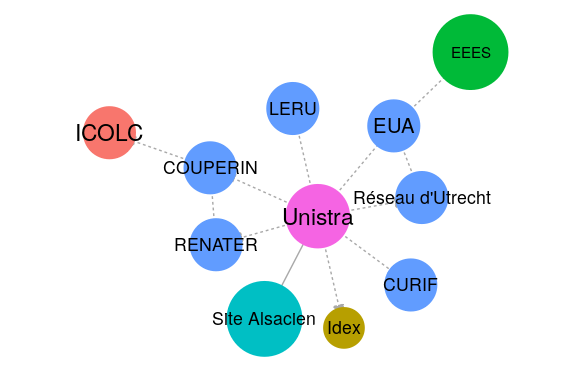
\includegraphics[width=1\linewidth,height=0.3\textheight]{tdbesr-rapport_files/figure-latex/unnamed-chunk-6-1} \end{center}

Exemple de lecture : « L'Université de Strasbourg (Unistra) a été créée
en 2009, par la fusion des universités Louis Pasteur, Robert Schuman et
Marc-Bloch. Ces trois universités ont été créées en 1970, par la
division de l'Université de Strasbourg (Académia argentinensis), dont
les origines remontent à 1528. »

\hypertarget{diagramme-dassociation}{%
\subsubsection{Diagramme d'association}\label{diagramme-dassociation}}

\begin{center}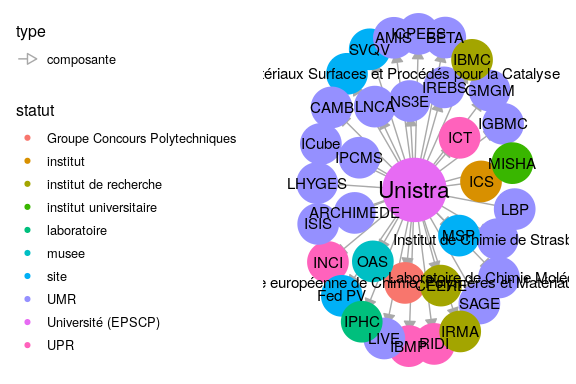
\includegraphics[width=1\linewidth,height=0.3\textheight]{tdbesr-rapport_files/figure-latex/unnamed-chunk-7-1} \end{center}

Exemple de lecture : « L'Université de Strasbourg (Unistra) est inclue
dans le Site Alsacien. Elle est membre de la LERU, de la CURIF, de
l'EUA, du Réseau d'Utrecht, de COUPERIN et de RENATER. Elle est
également lauréate de l'IDEX»

\hypertarget{diagramme-de-composition}{%
\subsubsection{Diagramme de
composition}\label{diagramme-de-composition}}

\begin{center}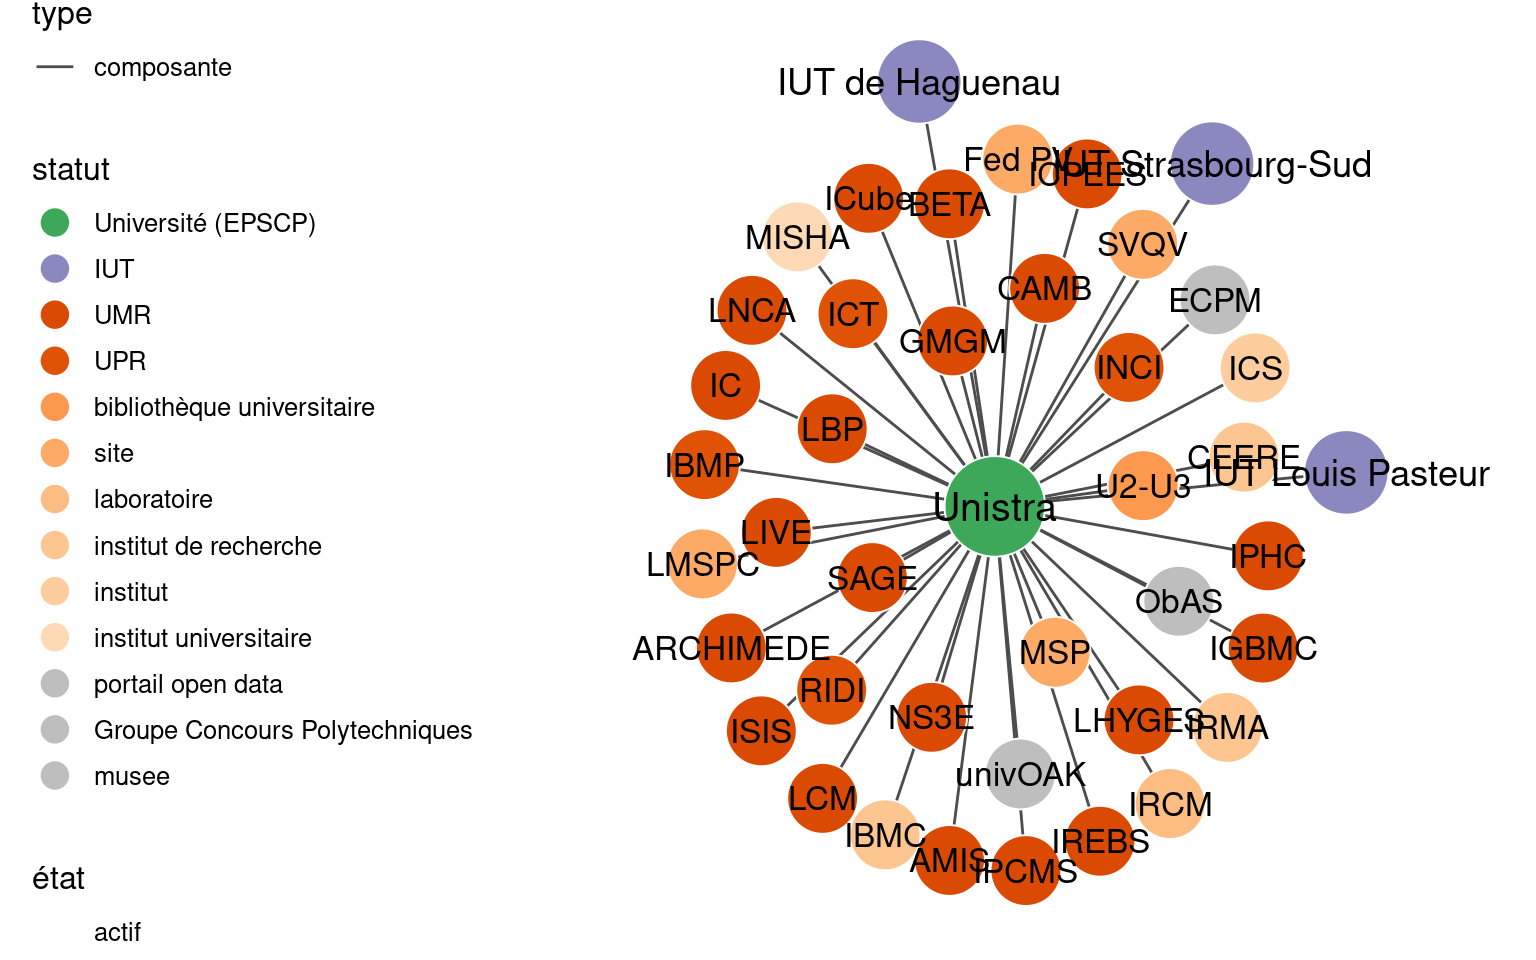
\includegraphics[width=1\linewidth,height=0.3\textheight]{tdbesr-rapport_files/figure-latex/unnamed-chunk-8-1} \end{center}

Exemple de lecture : « L'Université de Strasbourg (Unistra) a de
nombreuses composantes. »

\hypertarget{edition-collaborative}{%
\subsection{Edition collaborative}\label{edition-collaborative}}

Ces diagrammes dépendent d'une édition collaborative. En conséquence,
ils peuvent comporter des informations fausses, mais plus généralement
incomplètes et non uniformes.

Ce document fait partie d'un effort d'harmonisation de ces données,
grâce à une modélisation décrite dans
\href{https://github.com/cpesr/wikidataESR/blob/master/Rmd/wikidataESR.md}{ce
guide}. Chaque tableau de bord comporte un lien permettant de modifier
directement les informations sur WikiData.

Le lecteur est invité à le faire chaque fois qu'il le jugera nécessaire,
et les modifications seront automatiquement incluse dans la prochaine
version de ce document.

\hypertarget{indicateurs-de-performance}{%
\section{Indicateurs de performance}\label{indicateurs-de-performance}}

Dans ce travail, les indicateurs retenus sont de trois ordres~:
effectifs étudiants, effectifs enseignants et données financières. Il
n'existe malheureusement pas de données ouvertes sur les personnels
administratifs.

Ces indicateurs sont déclinés en deux types :

\begin{itemize}
\tightlist
\item
  les indicateurs primaires, secondaires et normalisés, au plus proche
  des jeux de données ouvertes ;
\item
  les indicateurs clés de performance, combinaison des précédents plus
  proche des missions.
\end{itemize}

\hypertarget{les-indicateurs-primaires-secondaires-et-normalisuxe9s}{%
\subsection{Les indicateurs primaires, secondaires et
normalisés}\label{les-indicateurs-primaires-secondaires-et-normalisuxe9s}}

Les indicateurs primaires et secondaires sont ceux qui sont directement
disponibles dans les jeux de données. L'indicateur primaire est le plus
général possible. Les indicateurs secondaires sont plus précis, et
peuvent se recouper (i.e.~la somme des indicateurs secondaires ne
correspond pas à l'indicateur principal).

Leur présentation est en deux volets. Le premier présente les valeurs
brutes, avec en première colonne l'indicateur primaire, et ensuite les
indicateurs secondaires.

Le second volet présente les valeurs normalisées, qui sont calculées
comme le rapport entre les indicateurs secondaires et l'indicateur
primaire. L'avantage principal de ces valeurs relatives est d'être
comparables d'un établissement à l'autre. On peut donc présenter la
moyenne de tous les établissements et leur distribution, afin d'y situer
chaque établissement.

Les indicateurs primaires suivant sont extraits des jeux de données
ouverts :

\begin{itemize}
\tightlist
\item
  \href{https://data.enseignementsup-recherche.gouv.fr/explore/dataset/fr-esr-principaux-etablissements-enseignement-superieur/}{Principaux
  établissements d'enseignement supérieur (lien)}

  \begin{itemize}
  \tightlist
  \item
    \textbf{UAI} : Unité Administrative Immatriculée
  \item
    \textbf{Libellé} et \textbf{Sigle}
  \item
    \textbf{Type} : université, regroupement ou autre
  \item
    \textbf{Type détaillé} : type d'établissement tel qu'il apparait
    dans le jeu de données
  \item
    \textbf{Académie}
  \item
    \textbf{Rattachement} : établissement de rattachement (regroupement
    et fusions)
  \item
    \textbf{Site web}, url \textbf{wikidata} et \textbf{légifrance}
  \end{itemize}
\item
  \href{https://data.enseignementsup-recherche.gouv.fr/explore/dataset/fr-esr-operateurs-indicateurs-financiers/}{Indicateurs
  financiers des opérateurs de l'enseignement supérieur français (lien)}

  \begin{itemize}
  \tightlist
  \item
    \textbf{Ressources} : \emph{Produits encaissables} dans le jeu de
    données
  \item
    \textbf{Masse salariale} : \emph{Dépenses de personnel} dans le jeu
    de données
  \item
    \textbf{Ressources propres} : \emph{Ressources propres / Produits
    encaissables} dans le jeu de données
  \end{itemize}
\item
  \href{https://data.enseignementsup-recherche.gouv.fr/explore/dataset/fr-esr-statistiques-sur-les-effectifs-d-etudiants-inscrits-par-etablissement/}{Statistiques
  sur les effectifs d'étudiants inscrits par établissement public sous
  tutelle du ministère en charge de l'Enseignement supérieur (lien)}

  \begin{itemize}
  \tightlist
  \item
    \textbf{Effectif étudiant} : Nombre d'étudiants inscrits
    (inscriptions principales) hors étudiants inscrits en parallèle en
    CPGE
  \item
    \textbf{Nombre d'inscriptions en Cycle 1 (L)} hors étudiants
    inscrits en parallèle en CPGE, inclu les DUT et autres formations
    post-bac
  \item
    \textbf{Nombre d'inscriptions en Cycle 2 (M)}
  \item
    \textbf{Nombre d'inscriptions en Cycle D (D)}
  \item
    \textbf{Nombre d'inscriptions en diplôme d'établissement} : par
    exemple diplôme d'université (DU)
  \end{itemize}
\item
  \href{https://data.enseignementsup-recherche.gouv.fr/explore/dataset/fr-esr-enseignants-titulaires-esr-public/}{Les
  enseignants titulaires dans les établissements publics de
  l'enseignement supérieur (lien)}
\item
  \href{https://data.enseignementsup-recherche.gouv.fr/explore/dataset/fr-esr-enseignants-nonpermanents-esr-public/}{Les
  enseignants non permanents des établissements publics de
  l'enseignement supérieur (lien)}

  \begin{itemize}
  \tightlist
  \item
    \textbf{Effectif enseignant} : les vacataires ne sont pas
    comptablisés et les quotités ne sont pas prises en compte
  \item
    \textbf{Effectif titulaire}
  \item
    \textbf{Enseignant-chercheurs titulaires}
  \item
    \textbf{Doctorants et ATER}
  \item
    \textbf{Contrats LRU}
  \end{itemize}
\end{itemize}

\hypertarget{les-indicateurs-cluxe9s-de-performance-kpi}{%
\subsection{Les indicateurs clés de performance
(KPI)}\label{les-indicateurs-cluxe9s-de-performance-kpi}}

Sur la base des indicateurs primaires, des indicateurs clés peuvent être
consruits pour représenter des informations plus proches des missions,
et donc plus à même de faire sens. Quatre indicateurs clés sont
présentés dans le cadre de ce travail~:

\begin{itemize}
\tightlist
\item
  \textbf{Taux de ressources propres}~: ce pourcentage des ressources
  qui ne proviennent pas de l'Etat permet de mesurer l'autonomie
  financère de l'établissement vis-à-vis de se tutelle principale.
  \emph{Attention}~: ce gain d'autonomie peut être compensée par une
  perte d'autonomie vis-à-vis d'autres acteurs.
\item
  \textbf{Taux de ressources par étudiant}~: ce rapport entre les
  ressources de l'établissement et le nombre d'étudiants inscrits en
  premier et deuxième cycle (L et M) permet de mesurer les ressources
  dont dispose l'établissement par rapport à la taille de sa population
  étudiante. \emph{Attention}~: ce taux ne correspond pas à la dépense
  de l'établissement pour chacun de ses étudiants \footnote{les dépenses
    sont multiples, et un établissement «~riche~» peut très bien
    consacrer son budget à d'autres fonction que l'enseignement. La
    comptabilité analytique interne aux établissements permet
    d'approcher une valeur de la dépense par étudiant, mais elle est
    généralement très peu fiable}.
\item
  \textbf{Taux d'encadrement}~: ce nombre d'enseignants titulaires pour
  100 étudiants inscrits en premier et deuxième cycle (L et M) permet de
  mesurer à la fois la qualité de l'encadrement, et la charge des
  enseignants. \emph{Attention}~: la répartition de cette charge peut
  être très hétérogène au sein même d'un établissement, tant entre les
  enseignants qu'entre les étudiants.
\item
  \textbf{Taux de titularité}~: pourcentage d'enseignants titulaires
  parmis tous les enseignants. \emph{Attention}~: il existe une
  population d'enseignants non titulaires «~normale~» \footnote{Par
    exemple~: doctorants et ATER, ou les vacataires professionnels qui
    ne relèvent pas d'une politique de précarisation}, ce n'est donc pas
  une mesure directe de la précarité enseignante.
\end{itemize}

Les indicateurs clés de performances sont présentés sous trois formes :

\begin{itemize}
\tightlist
\item
  Normalisés : les valeurs de la dernière année sont présentées en
  fonction de la moyenne nationale des établissements de même type ;
\item
  Evolution en valeur absolue : les valeurs sont présentées sur
  plusieurs années ;
\item
  Evolution en valeur de référence : les valeurs sont présentées en
  pourcentage relatif à l'année de référence.
\end{itemize}

Pour chacune des trois présentations, le fond de graphique représente
les valeurs de tous les autres établissements, sous forme de point (un
point par établissement), de
\href{https://fr.wikipedia.org/wiki/Bo\%C3\%AEte_\%C3\%A0_moustaches}{boite
à moustaches}, ou de distribution en violon.

\hypertarget{exemples-de-lecture}{%
\subsection{Exemples de lecture}\label{exemples-de-lecture}}

\hypertarget{kpi-normalisuxe9s}{%
\subsubsection{KPI : normalisés}\label{kpi-normalisuxe9s}}

\begin{center}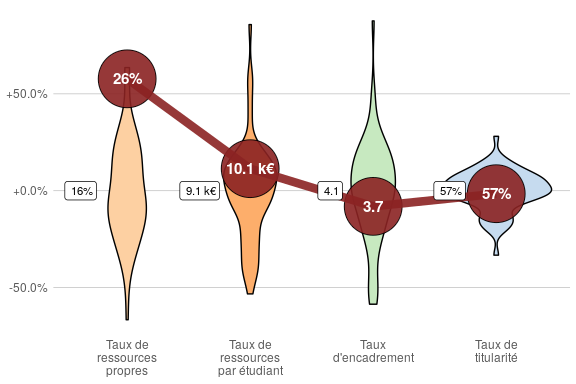
\includegraphics[width=1\linewidth,height=0.3\textheight]{tdbesr-rapport_files/figure-latex/kpi.raw-1} \end{center}

Exemple de lecture : « Le taux de titularité de cet établissement est de
3,7, pour une moyenne nationale de 4,1. ».

\hypertarget{kpi-uxe9volution-en-valeur-absolue}{%
\subsubsection{KPI : évolution en valeur
absolue}\label{kpi-uxe9volution-en-valeur-absolue}}

\begin{center}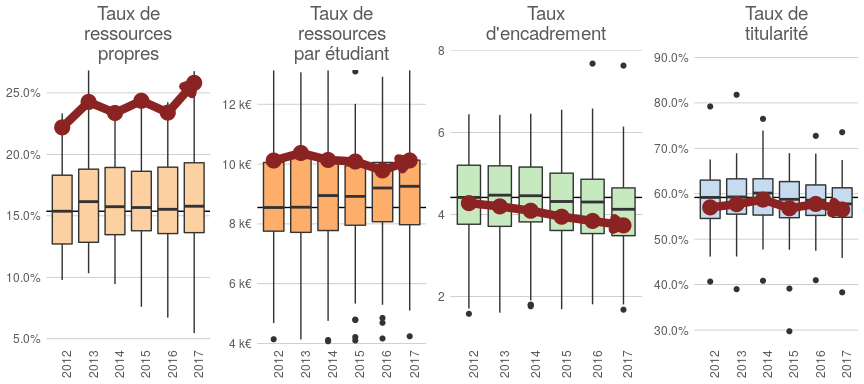
\includegraphics[width=1\linewidth,height=0.3\textheight]{tdbesr-rapport_files/figure-latex/kpi.evol.raw-1} \end{center}

Exemple de lecture : « En 2012, le taux d'encadrement de l'établissement
était à 4,3, soit la médiane pour toutes les universités. Il est
progressivement passé à 3,7, ce qui place maintenant l'établissement
dans le deuxième quartile ».

\hypertarget{kpi-uxe9volution-en-valeur-de-ruxe9fuxe9rence}{%
\subsubsection{KPI : évolution en valeur de
référence}\label{kpi-uxe9volution-en-valeur-de-ruxe9fuxe9rence}}

\begin{center}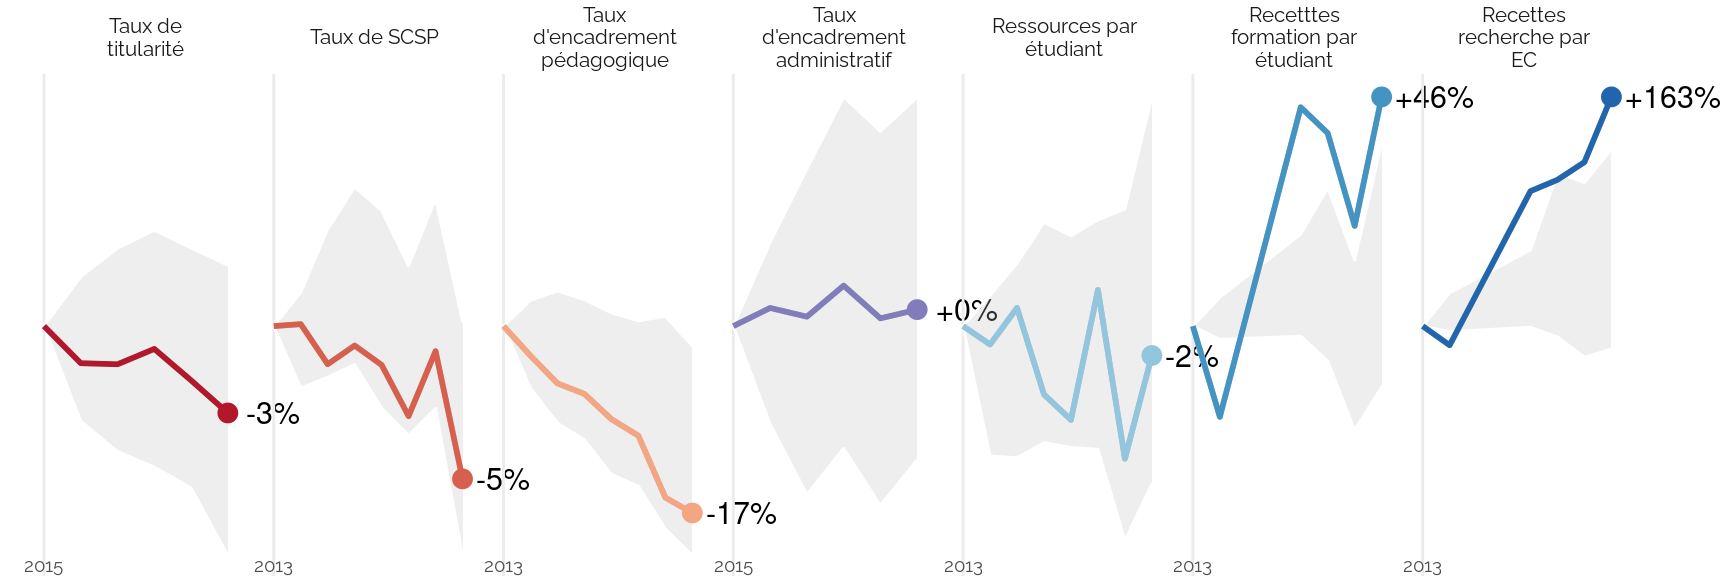
\includegraphics[width=1\linewidth,height=0.3\textheight]{tdbesr-rapport_files/figure-latex/kpi.evol.nor-1} \end{center}

Exemple de lecture : « Entre 2012 et 2017, le taux d'encadrement de
l'établissement a baissé d'environ 15\%, ce qui le place dans le premier
quartile inférieur des évolution de cet indicateur ».

\hypertarget{donnuxe9es-brutes}{%
\subsubsection{Données brutes}\label{donnuxe9es-brutes}}

\begin{center}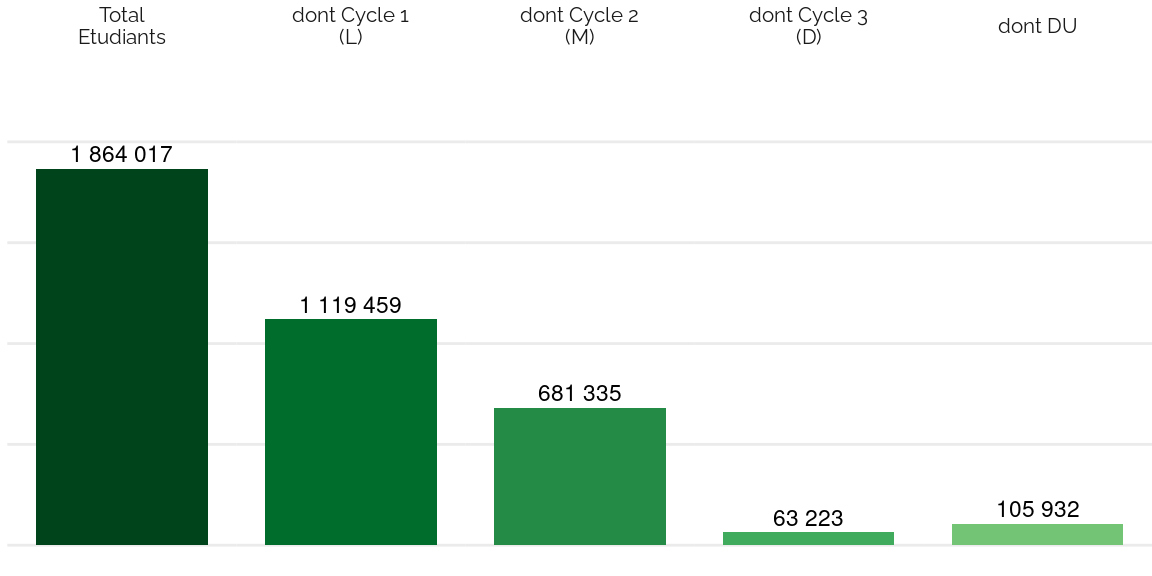
\includegraphics[width=1\linewidth,height=0.3\textheight]{tdbesr-rapport_files/figure-latex/etu.raw-1} \end{center}

Exemple de lecture : « l'établissement compte 47 573 étudiants hors
double inscription en CPGE, dont 26 679 en 1er cycle (L, DUT, prépa,
etc.) ».

\hypertarget{donnuxe9es-normalisuxe9es}{%
\subsubsection{Données normalisées}\label{donnuxe9es-normalisuxe9es}}

\begin{center}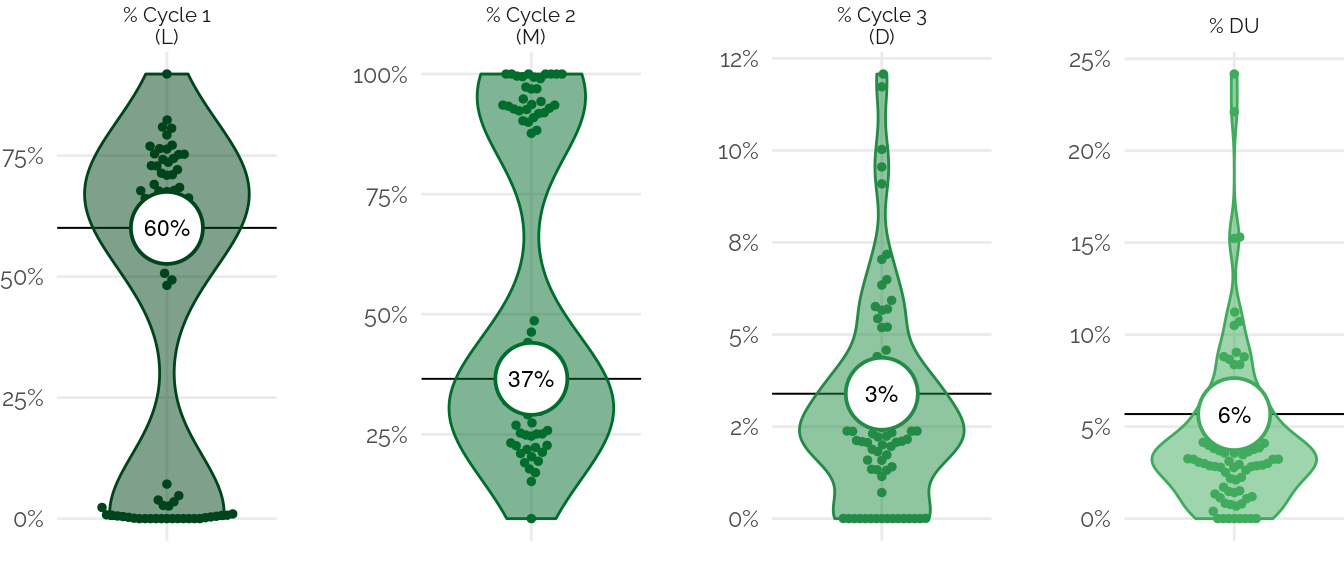
\includegraphics[width=1\linewidth,height=0.3\textheight]{tdbesr-rapport_files/figure-latex/etu.norm-1} \end{center}

Exemple de lecture : « La part moyenne des étudiants en 1er cycle dans
les effectifs des universités est de 68\%. L'établissement présente une
part de 56\%, ce qui le place dans le quartile inférieur ».

\end{multicols}
%\begin{changemargin}{-1cm}{-1cm}

\newpage
\scriptsize

\newpage   
\vspace*{5cm}   
\part{Type d'établissement :  Université }   
\newpage

\hypertarget{acaduxe9mie-aix-marseille}{%
\section{Académie : Aix-Marseille}\label{acaduxe9mie-aix-marseille}}

\hypertarget{aix-marseille-universituxe9-amu}{%
\subsection{Aix-Marseille Université
(AMU)}\label{aix-marseille-universituxe9-amu}}

\begin{tabular*}{0.45\textwidth}{rp{2cm}rl}  
\hline  
Type : & Université & Web : &\href{http://www.univ-amu.fr/}{http://www.univ-amu.fr/} \\  
Rattachement : & N/A & Wikidata : & \href{https://www.wikidata.org/entity/Q2302586}{Q2302586} \\  
UAI : & 0134009M & Décret : & N/A \\  
\hline  
\end{tabular*}

\textit{\scriptsize Pour améliorer ces graphiques, veuillez éditer \href{https://www.wikidata.org/entity/Q2302586}{Q2302586}  selon \href{https://github.com/cpesr/wikidataESR/blob/master/Rmd/wikidataESR.md}{ce guide}}
.

\maketdb{tdbesr-batch/0134009M-filiation}{tdbesr-batch/0134009M-association}{tdbesr-batch/0134009M-composition}{tdbesr-batch/0134009M-kpi}

\newpage

\hypertarget{avignon-universituxe9-au}{%
\subsection{Avignon Université (AU)}\label{avignon-universituxe9-au}}

\begin{tabular*}{0.45\textwidth}{rp{2cm}rl}  
\hline  
Type : & Université & Web : &\href{http://www.univ-avignon.fr/}{http://www.univ-avignon.fr/} \\  
Rattachement : & N/A & Wikidata : & \href{https://www.wikidata.org/entity/Q2033119}{Q2033119} \\  
UAI : & 0840685N & Décret : & N/A \\  
\hline  
\end{tabular*}

\textit{\scriptsize Pour améliorer ces graphiques, veuillez éditer \href{https://www.wikidata.org/entity/Q2033119}{Q2033119}  selon \href{https://github.com/cpesr/wikidataESR/blob/master/Rmd/wikidataESR.md}{ce guide}}
.

\maketdb{tdbesr-batch/0840685N-filiation}{tdbesr-batch/0840685N-association}{tdbesr-batch/0840685N-composition}{tdbesr-batch/0840685N-kpi}

\newpage

\hypertarget{acaduxe9mie-amiens}{%
\section{Académie : Amiens}\label{acaduxe9mie-amiens}}

\hypertarget{universituxe9-de-picardie-jules-verne-upjv}{%
\subsection{Université de Picardie Jules-Verne
(UPJV)}\label{universituxe9-de-picardie-jules-verne-upjv}}

\begin{tabular*}{0.45\textwidth}{rp{2cm}rl}  
\hline  
Type : & Université & Web : &\href{http://www.u-picardie.fr/}{http://www.u-picardie.fr/} \\  
Rattachement : & N/A & Wikidata : & \href{https://www.wikidata.org/entity/Q947747}{Q947747} \\  
UAI : & 0801344B & Décret : & N/A \\  
\hline  
\end{tabular*}

\textit{\scriptsize Pour améliorer ces graphiques, veuillez éditer \href{https://www.wikidata.org/entity/Q947747}{Q947747}  selon \href{https://github.com/cpesr/wikidataESR/blob/master/Rmd/wikidataESR.md}{ce guide}}
.

\maketdb{tdbesr-batch/0801344B-filiation}{tdbesr-batch/0801344B-association}{tdbesr-batch/0801344B-composition}{tdbesr-batch/0801344B-kpi}

\newpage

\hypertarget{acaduxe9mie-besanuxe7on}{%
\section{Académie : Besançon}\label{acaduxe9mie-besanuxe7on}}

\hypertarget{universituxe9-de-franche-comtuxe9-ufc}{%
\subsection{Université de Franche-Comté
(UFC)}\label{universituxe9-de-franche-comtuxe9-ufc}}

\begin{tabular*}{0.45\textwidth}{rp{2cm}rl}  
\hline  
Type : & Université & Web : &\href{http://www.univ-fcomte.fr/}{http://www.univ-fcomte.fr/} \\  
Rattachement : & N/A & Wikidata : & \href{https://www.wikidata.org/entity/Q829449}{Q829449} \\  
UAI : & 0251215K & Décret : & N/A \\  
\hline  
\end{tabular*}

\textit{\scriptsize Pour améliorer ces graphiques, veuillez éditer \href{https://www.wikidata.org/entity/Q829449}{Q829449}  selon \href{https://github.com/cpesr/wikidataESR/blob/master/Rmd/wikidataESR.md}{ce guide}}
.

\maketdb{tdbesr-batch/0251215K-filiation}{tdbesr-batch/0251215K-association}{tdbesr-batch/0251215K-composition}{tdbesr-batch/0251215K-kpi}

\newpage

\hypertarget{acaduxe9mie-bordeaux}{%
\section{Académie : Bordeaux}\label{acaduxe9mie-bordeaux}}

\hypertarget{universituxe9-bordeaux-montaigne-ubm}{%
\subsection{Université Bordeaux-Montaigne
(UBM)}\label{universituxe9-bordeaux-montaigne-ubm}}

\begin{tabular*}{0.45\textwidth}{rp{2cm}rl}  
\hline  
Type : & Université & Web : &\href{http://www.u-bordeaux-montaigne.fr/}{http://www.u-bordeaux-montaigne.fr/} \\  
Rattachement : & N/A & Wikidata : & \href{https://www.wikidata.org/entity/Q13342}{Q13342} \\  
UAI : & 0331766R & Décret : & N/A \\  
\hline  
\end{tabular*}

\textit{\scriptsize Pour améliorer ces graphiques, veuillez éditer \href{https://www.wikidata.org/entity/Q13342}{Q13342}  selon \href{https://github.com/cpesr/wikidataESR/blob/master/Rmd/wikidataESR.md}{ce guide}}
.

\maketdb{tdbesr-batch/0331766R-filiation}{tdbesr-batch/0331766R-association}{tdbesr-batch/0331766R-composition}{tdbesr-batch/0331766R-kpi}

\newpage

\hypertarget{universituxe9-de-bordeaux-na}{%
\subsection{Université de Bordeaux
(N/A)}\label{universituxe9-de-bordeaux-na}}

\begin{tabular*}{0.45\textwidth}{rp{2cm}rl}  
\hline  
Type : & Université & Web : &\href{http://www.u-bordeaux.fr/}{http://www.u-bordeaux.fr/} \\  
Rattachement : & N/A & Wikidata : & \href{https://www.wikidata.org/entity/Q13344}{Q13344} \\  
UAI : & 0333298F & Décret : & N/A \\  
\hline  
\end{tabular*}

\textit{\scriptsize Pour améliorer ces graphiques, veuillez éditer \href{https://www.wikidata.org/entity/Q13344}{Q13344}  selon \href{https://github.com/cpesr/wikidataESR/blob/master/Rmd/wikidataESR.md}{ce guide}}
.

\maketdb{tdbesr-batch/0333298F-filiation}{tdbesr-batch/0333298F-association}{tdbesr-batch/0333298F-composition}{tdbesr-batch/0333298F-kpi}

\newpage

\hypertarget{universituxe9-de-pau-et-des-pays-de-ladour-uppa}{%
\subsection{Université de Pau et des Pays de l'Adour
(UPPA)}\label{universituxe9-de-pau-et-des-pays-de-ladour-uppa}}

\begin{tabular*}{0.45\textwidth}{rp{2cm}rl}  
\hline  
Type : & Université & Web : &\href{http://www.univ-pau.fr/}{http://www.univ-pau.fr/} \\  
Rattachement : & N/A & Wikidata : & \href{https://www.wikidata.org/entity/Q572968}{Q572968} \\  
UAI : & 0640251A & Décret : & N/A \\  
\hline  
\end{tabular*}

\textit{\scriptsize Pour améliorer ces graphiques, veuillez éditer \href{https://www.wikidata.org/entity/Q572968}{Q572968}  selon \href{https://github.com/cpesr/wikidataESR/blob/master/Rmd/wikidataESR.md}{ce guide}}
.

\maketdb{tdbesr-batch/0640251A-filiation}{tdbesr-batch/0640251A-association}{tdbesr-batch/0640251A-composition}{tdbesr-batch/0640251A-kpi}

\newpage

\hypertarget{acaduxe9mie-clermont-ferrand}{%
\section{Académie :
Clermont-Ferrand}\label{acaduxe9mie-clermont-ferrand}}

\hypertarget{universituxe9-clermont-auvergne-uca}{%
\subsection{Université Clermont Auvergne
(UCA)}\label{universituxe9-clermont-auvergne-uca}}

\begin{tabular*}{0.45\textwidth}{rp{2cm}rl}  
\hline  
Type : & Université & Web : &\href{https://www.uca.fr/}{https://www.uca.fr/} \\  
Rattachement : & N/A & Wikidata : & \href{https://www.wikidata.org/entity/Q28057967}{Q28057967} \\  
UAI : & 0632035V & Décret : & \href{https://www.legifrance.gouv.fr/affichTexte.do?cidTexte=JORFTEXT000033119145&categorieLien=id}{Legifrance} \\  
\hline  
\end{tabular*}

\textit{\scriptsize Pour améliorer ces graphiques, veuillez éditer \href{https://www.wikidata.org/entity/Q28057967}{Q28057967}  selon \href{https://github.com/cpesr/wikidataESR/blob/master/Rmd/wikidataESR.md}{ce guide}}
.

\maketdb{tdbesr-batch/0632035V-filiation}{tdbesr-batch/0632035V-association}{tdbesr-batch/0632035V-composition}{tdbesr-batch/0632035V-kpi}

\newpage

\hypertarget{acaduxe9mie-corse}{%
\section{Académie : Corse}\label{acaduxe9mie-corse}}

\hypertarget{universituxe9-de-corse-pasquale-paoli-na}{%
\subsection{Université de Corse Pasquale Paoli
(N/A)}\label{universituxe9-de-corse-pasquale-paoli-na}}

\begin{tabular*}{0.45\textwidth}{rp{2cm}rl}  
\hline  
Type : & Université & Web : &\href{https://www.universita.corsica/fr/}{https://www.universita.corsica/fr/} \\  
Rattachement : & N/A & Wikidata : & \href{https://www.wikidata.org/entity/Q335841}{Q335841} \\  
UAI : & 7200664J & Décret : & N/A \\  
\hline  
\end{tabular*}

\textit{\scriptsize Pour améliorer ces graphiques, veuillez éditer \href{https://www.wikidata.org/entity/Q335841}{Q335841}  selon \href{https://github.com/cpesr/wikidataESR/blob/master/Rmd/wikidataESR.md}{ce guide}}
.

\maketdb{tdbesr-batch/7200664J-filiation}{tdbesr-batch/7200664J-association}{tdbesr-batch/7200664J-composition}{tdbesr-batch/7200664J-kpi}

\newpage

\hypertarget{acaduxe9mie-cruxe9teil}{%
\section{Académie : Créteil}\label{acaduxe9mie-cruxe9teil}}

\hypertarget{universituxe9-sorbonne-paris-nord-na}{%
\subsection{Université Sorbonne Paris Nord
(N/A)}\label{universituxe9-sorbonne-paris-nord-na}}

\begin{tabular*}{0.45\textwidth}{rp{2cm}rl}  
\hline  
Type : & Université & Web : &\href{http://www.univ-paris13.fr/}{http://www.univ-paris13.fr/} \\  
Rattachement : & N/A & Wikidata : & \href{https://www.wikidata.org/entity/Q1780212}{Q1780212} \\  
UAI : & 0931238R & Décret : & N/A \\  
\hline  
\end{tabular*}

\textit{\scriptsize Pour améliorer ces graphiques, veuillez éditer \href{https://www.wikidata.org/entity/Q1780212}{Q1780212}  selon \href{https://github.com/cpesr/wikidataESR/blob/master/Rmd/wikidataESR.md}{ce guide}}
.

\maketdb{tdbesr-batch/0931238R-filiation}{tdbesr-batch/0931238R-association}{tdbesr-batch/0931238R-composition}{tdbesr-batch/0931238R-kpi}

\newpage

\hypertarget{universituxe9-paris-8---vincennes---saint-denis-na}{%
\subsection{Université Paris 8 - Vincennes - Saint-Denis
(N/A)}\label{universituxe9-paris-8---vincennes---saint-denis-na}}

\begin{tabular*}{0.45\textwidth}{rp{2cm}rl}  
\hline  
Type : & Université & Web : &\href{http://www.univ-paris8.fr/}{http://www.univ-paris8.fr/} \\  
Rattachement : & N/A & Wikidata : & \href{https://www.wikidata.org/entity/Q1194988}{Q1194988} \\  
UAI : & 0931827F & Décret : & N/A \\  
\hline  
\end{tabular*}

\textit{\scriptsize Pour améliorer ces graphiques, veuillez éditer \href{https://www.wikidata.org/entity/Q1194988}{Q1194988}  selon \href{https://github.com/cpesr/wikidataESR/blob/master/Rmd/wikidataESR.md}{ce guide}}
.

\maketdb{tdbesr-batch/0931827F-filiation}{tdbesr-batch/0931827F-association}{tdbesr-batch/0931827F-composition}{tdbesr-batch/0931827F-kpi}

\newpage

\hypertarget{universituxe9-paris-est-cruxe9teil-val-de-marne-upec}{%
\subsection{Université Paris-Est Créteil Val-de-Marne
(UPEC)}\label{universituxe9-paris-est-cruxe9teil-val-de-marne-upec}}

\begin{tabular*}{0.45\textwidth}{rp{2cm}rl}  
\hline  
Type : & Université & Web : &\href{http://www.u-pec.fr/}{http://www.u-pec.fr/} \\  
Rattachement : & N/A & Wikidata : & \href{https://www.wikidata.org/entity/Q980688}{Q980688} \\  
UAI : & 0941111X & Décret : & N/A \\  
\hline  
\end{tabular*}

\textit{\scriptsize Pour améliorer ces graphiques, veuillez éditer \href{https://www.wikidata.org/entity/Q980688}{Q980688}  selon \href{https://github.com/cpesr/wikidataESR/blob/master/Rmd/wikidataESR.md}{ce guide}}
.

\maketdb{tdbesr-batch/0941111X-filiation}{tdbesr-batch/0941111X-association}{tdbesr-batch/0941111X-composition}{tdbesr-batch/0941111X-kpi}

\newpage

\hypertarget{acaduxe9mie-dijon}{%
\section{Académie : Dijon}\label{acaduxe9mie-dijon}}

\hypertarget{universituxe9-de-bourgogne-na}{%
\subsection{Université de Bourgogne
(N/A)}\label{universituxe9-de-bourgogne-na}}

\begin{tabular*}{0.45\textwidth}{rp{2cm}rl}  
\hline  
Type : & Université & Web : &\href{http://www.u-bourgogne.fr/}{http://www.u-bourgogne.fr/} \\  
Rattachement : & N/A & Wikidata : & \href{https://www.wikidata.org/entity/Q287072}{Q287072} \\  
UAI : & 0211237F & Décret : & N/A \\  
\hline  
\end{tabular*}

\textit{\scriptsize Pour améliorer ces graphiques, veuillez éditer \href{https://www.wikidata.org/entity/Q287072}{Q287072}  selon \href{https://github.com/cpesr/wikidataESR/blob/master/Rmd/wikidataESR.md}{ce guide}}
.

\maketdb{tdbesr-batch/0211237F-filiation}{tdbesr-batch/0211237F-association}{tdbesr-batch/0211237F-composition}{tdbesr-batch/0211237F-kpi}

\newpage

\hypertarget{acaduxe9mie-grenoble}{%
\section{Académie : Grenoble}\label{acaduxe9mie-grenoble}}

\hypertarget{universituxe9-savoie-mont-blanc-usmb}{%
\subsection{Université Savoie Mont Blanc
(USMB)}\label{universituxe9-savoie-mont-blanc-usmb}}

\begin{tabular*}{0.45\textwidth}{rp{2cm}rl}  
\hline  
Type : & Université & Web : &\href{http://www.univ-savoie.fr/}{http://www.univ-savoie.fr/} \\  
Rattachement : & N/A & Wikidata : & \href{https://www.wikidata.org/entity/Q2496158}{Q2496158} \\  
UAI : & 0730858L & Décret : & N/A \\  
\hline  
\end{tabular*}

\textit{\scriptsize Pour améliorer ces graphiques, veuillez éditer \href{https://www.wikidata.org/entity/Q2496158}{Q2496158}  selon \href{https://github.com/cpesr/wikidataESR/blob/master/Rmd/wikidataESR.md}{ce guide}}
.

\maketdb{tdbesr-batch/0730858L-filiation}{tdbesr-batch/0730858L-association}{tdbesr-batch/0730858L-composition}{tdbesr-batch/0730858L-kpi}

\newpage

\hypertarget{acaduxe9mie-guadeloupe}{%
\section{Académie : Guadeloupe}\label{acaduxe9mie-guadeloupe}}

\hypertarget{universituxe9-des-antilles-na}{%
\subsection{Université des Antilles
(N/A)}\label{universituxe9-des-antilles-na}}

\begin{tabular*}{0.45\textwidth}{rp{2cm}rl}  
\hline  
Type : & Université & Web : &\href{http://www.univ-ag.fr/}{http://www.univ-ag.fr/} \\  
Rattachement : & N/A & Wikidata : & \href{https://www.wikidata.org/entity/Q829169}{Q829169} \\  
UAI : & 9710585J & Décret : & N/A \\  
\hline  
\end{tabular*}

\textit{\scriptsize Pour améliorer ces graphiques, veuillez éditer \href{https://www.wikidata.org/entity/Q829169}{Q829169}  selon \href{https://github.com/cpesr/wikidataESR/blob/master/Rmd/wikidataESR.md}{ce guide}}
.

\maketdb{tdbesr-batch/9710585J-filiation}{tdbesr-batch/9710585J-association}{tdbesr-batch/9710585J-composition}{tdbesr-batch/9710585J-kpi}

\newpage

\hypertarget{acaduxe9mie-guyane}{%
\section{Académie : Guyane}\label{acaduxe9mie-guyane}}

\hypertarget{universituxe9-de-guyane-na}{%
\subsection{Université de Guyane
(N/A)}\label{universituxe9-de-guyane-na}}

\begin{tabular*}{0.45\textwidth}{rp{2cm}rl}  
\hline  
Type : & Université & Web : &\href{http://www.univ-guyane.fr/}{http://www.univ-guyane.fr/} \\  
Rattachement : & N/A & Wikidata : & \href{https://www.wikidata.org/entity/Q16682067}{Q16682067} \\  
UAI : & 9730429D & Décret : & \href{http://www.legifrance.gouv.fr/affichTexte.do;jsessionid=?cidTexte=JORFTEXT000029310823&dateTexte=&oldAction=dernierJO&categorieLien=id}{Legifrance} \\  
\hline  
\end{tabular*}

\textit{\scriptsize Pour améliorer ces graphiques, veuillez éditer \href{https://www.wikidata.org/entity/Q16682067}{Q16682067}  selon \href{https://github.com/cpesr/wikidataESR/blob/master/Rmd/wikidataESR.md}{ce guide}}
.

\maketdb{tdbesr-batch/9730429D-filiation}{tdbesr-batch/9730429D-association}{tdbesr-batch/9730429D-composition}{tdbesr-batch/9730429D-kpi}

\newpage

\hypertarget{acaduxe9mie-la-ruxe9union}{%
\section{Académie : La Réunion}\label{acaduxe9mie-la-ruxe9union}}

\hypertarget{universituxe9-de-la-ruxe9union-na}{%
\subsection{Université de La Réunion
(N/A)}\label{universituxe9-de-la-ruxe9union-na}}

\begin{tabular*}{0.45\textwidth}{rp{2cm}rl}  
\hline  
Type : & Université & Web : &\href{http://www.univ-reunion.fr/}{http://www.univ-reunion.fr/} \\  
Rattachement : & N/A & Wikidata : & \href{https://www.wikidata.org/entity/Q834819}{Q834819} \\  
UAI : & 9740478B & Décret : & N/A \\  
\hline  
\end{tabular*}

\textit{\scriptsize Pour améliorer ces graphiques, veuillez éditer \href{https://www.wikidata.org/entity/Q834819}{Q834819}  selon \href{https://github.com/cpesr/wikidataESR/blob/master/Rmd/wikidataESR.md}{ce guide}}
.

\maketdb{tdbesr-batch/9740478B-filiation}{tdbesr-batch/9740478B-association}{tdbesr-batch/9740478B-composition}{tdbesr-batch/9740478B-kpi}

\newpage

\hypertarget{acaduxe9mie-lille}{%
\section{Académie : Lille}\label{acaduxe9mie-lille}}

\hypertarget{universituxe9-du-littoral-cuxf4te-dopale-ulco}{%
\subsection{Université du Littoral Côte d'Opale
(ULCO)}\label{universituxe9-du-littoral-cuxf4te-dopale-ulco}}

\begin{tabular*}{0.45\textwidth}{rp{2cm}rl}  
\hline  
Type : & Université & Web : &\href{http://www.univ-littoral.fr/}{http://www.univ-littoral.fr/} \\  
Rattachement : & N/A & Wikidata : & \href{https://www.wikidata.org/entity/Q3551755}{Q3551755} \\  
UAI : & 0595964M & Décret : & N/A \\  
\hline  
\end{tabular*}

\textit{\scriptsize Pour améliorer ces graphiques, veuillez éditer \href{https://www.wikidata.org/entity/Q3551755}{Q3551755}  selon \href{https://github.com/cpesr/wikidataESR/blob/master/Rmd/wikidataESR.md}{ce guide}}
.

\maketdb{tdbesr-batch/0595964M-filiation}{tdbesr-batch/0595964M-association}{tdbesr-batch/0595964M-composition}{tdbesr-batch/0595964M-kpi}

\newpage

\hypertarget{universituxe9-de-lille-na}{%
\subsection{Université de Lille (N/A)}\label{universituxe9-de-lille-na}}

\begin{tabular*}{0.45\textwidth}{rp{2cm}rl}  
\hline  
Type : & Université & Web : &\href{https://www.univ-lille.fr/}{https://www.univ-lille.fr/} \\  
Rattachement : & N/A & Wikidata : & \href{https://www.wikidata.org/entity/Q3551621}{Q3551621} \\  
UAI : & 0597065J & Décret : & \href{https://www.legifrance.gouv.fr/affichTexte.do?cidTexte=JORFTEXT000035543008}{Legifrance} \\  
\hline  
\end{tabular*}

\textit{\scriptsize Pour améliorer ces graphiques, veuillez éditer \href{https://www.wikidata.org/entity/Q3551621}{Q3551621}  selon \href{https://github.com/cpesr/wikidataESR/blob/master/Rmd/wikidataESR.md}{ce guide}}
.

\maketdb{tdbesr-batch/0597065J-filiation}{tdbesr-batch/0597065J-association}{tdbesr-batch/0597065J-composition}{tdbesr-batch/0597065J-kpi}

\newpage

\hypertarget{universituxe9-dartois-na}{%
\subsection{Université d'Artois (N/A)}\label{universituxe9-dartois-na}}

\begin{tabular*}{0.45\textwidth}{rp{2cm}rl}  
\hline  
Type : & Université & Web : &\href{http://www.univ-artois.fr/}{http://www.univ-artois.fr/} \\  
Rattachement : & N/A & Wikidata : & \href{https://www.wikidata.org/entity/Q475504}{Q475504} \\  
UAI : & 0623957P & Décret : & N/A \\  
\hline  
\end{tabular*}

\textit{\scriptsize Pour améliorer ces graphiques, veuillez éditer \href{https://www.wikidata.org/entity/Q475504}{Q475504}  selon \href{https://github.com/cpesr/wikidataESR/blob/master/Rmd/wikidataESR.md}{ce guide}}
.

\maketdb{tdbesr-batch/0623957P-filiation}{tdbesr-batch/0623957P-association}{tdbesr-batch/0623957P-composition}{tdbesr-batch/0623957P-kpi}

\newpage

\hypertarget{acaduxe9mie-limoges}{%
\section{Académie : Limoges}\label{acaduxe9mie-limoges}}

\hypertarget{universituxe9-de-limoges-na}{%
\subsection{Université de Limoges
(N/A)}\label{universituxe9-de-limoges-na}}

\begin{tabular*}{0.45\textwidth}{rp{2cm}rl}  
\hline  
Type : & Université & Web : &\href{http://www.unilim.fr/}{http://www.unilim.fr/} \\  
Rattachement : & N/A & Wikidata : & \href{https://www.wikidata.org/entity/Q2661290}{Q2661290} \\  
UAI : & 0870669E & Décret : & \href{https://www.legifrance.gouv.fr/eli/decret/2016/12/15/MENS1630827D/jo/texte/fr}{Legifrance} \\  
\hline  
\end{tabular*}

\textit{\scriptsize Pour améliorer ces graphiques, veuillez éditer \href{https://www.wikidata.org/entity/Q2661290}{Q2661290}  selon \href{https://github.com/cpesr/wikidataESR/blob/master/Rmd/wikidataESR.md}{ce guide}}
.

\maketdb{tdbesr-batch/0870669E-filiation}{tdbesr-batch/0870669E-association}{tdbesr-batch/0870669E-composition}{tdbesr-batch/0870669E-kpi}

\newpage

\hypertarget{acaduxe9mie-lyon}{%
\section{Académie : Lyon}\label{acaduxe9mie-lyon}}

\hypertarget{universituxe9-jean-monnet-na}{%
\subsection{Université Jean Monnet
(N/A)}\label{universituxe9-jean-monnet-na}}

\begin{tabular*}{0.45\textwidth}{rp{2cm}rl}  
\hline  
Type : & Université & Web : &\href{http://portail.univ-st-etienne.fr/}{http://portail.univ-st-etienne.fr/} \\  
Rattachement : & N/A & Wikidata : & \href{https://www.wikidata.org/entity/Q623154}{Q623154} \\  
UAI : & 0421095M & Décret : & N/A \\  
\hline  
\end{tabular*}

\textit{\scriptsize Pour améliorer ces graphiques, veuillez éditer \href{https://www.wikidata.org/entity/Q623154}{Q623154}  selon \href{https://github.com/cpesr/wikidataESR/blob/master/Rmd/wikidataESR.md}{ce guide}}
.

\maketdb{tdbesr-batch/0421095M-filiation}{tdbesr-batch/0421095M-association}{tdbesr-batch/0421095M-composition}{tdbesr-batch/0421095M-kpi}

\newpage

\hypertarget{universituxe9-claude-bernard---lyon-1-na}{%
\subsection{Université Claude Bernard - Lyon 1
(N/A)}\label{universituxe9-claude-bernard---lyon-1-na}}

\begin{tabular*}{0.45\textwidth}{rp{2cm}rl}  
\hline  
Type : & Université & Web : &\href{http://www.univ-lyon1.fr/}{http://www.univ-lyon1.fr/} \\  
Rattachement : & N/A & Wikidata : & \href{https://www.wikidata.org/entity/Q4032}{Q4032} \\  
UAI : & 0691774D & Décret : & N/A \\  
\hline  
\end{tabular*}

\textit{\scriptsize Pour améliorer ces graphiques, veuillez éditer \href{https://www.wikidata.org/entity/Q4032}{Q4032}  selon \href{https://github.com/cpesr/wikidataESR/blob/master/Rmd/wikidataESR.md}{ce guide}}
.

\maketdb{tdbesr-batch/0691774D-filiation}{tdbesr-batch/0691774D-association}{tdbesr-batch/0691774D-composition}{tdbesr-batch/0691774D-kpi}

\newpage

\hypertarget{universituxe9-lumiuxe8re---lyon-2-na}{%
\subsection{Université Lumière - Lyon 2
(N/A)}\label{universituxe9-lumiuxe8re---lyon-2-na}}

\begin{tabular*}{0.45\textwidth}{rp{2cm}rl}  
\hline  
Type : & Université & Web : &\href{http://www.univ-lyon2.fr/}{http://www.univ-lyon2.fr/} \\  
Rattachement : & N/A & Wikidata : & \href{https://www.wikidata.org/entity/Q4041}{Q4041} \\  
UAI : & 0691775E & Décret : & N/A \\  
\hline  
\end{tabular*}

\textit{\scriptsize Pour améliorer ces graphiques, veuillez éditer \href{https://www.wikidata.org/entity/Q4041}{Q4041}  selon \href{https://github.com/cpesr/wikidataESR/blob/master/Rmd/wikidataESR.md}{ce guide}}
.

\maketdb{tdbesr-batch/0691775E-filiation}{tdbesr-batch/0691775E-association}{tdbesr-batch/0691775E-composition}{tdbesr-batch/0691775E-kpi}

\newpage

\hypertarget{universituxe9-jean-moulin---lyon-3-na}{%
\subsection{Université Jean Moulin - Lyon 3
(N/A)}\label{universituxe9-jean-moulin---lyon-3-na}}

\begin{tabular*}{0.45\textwidth}{rp{2cm}rl}  
\hline  
Type : & Université & Web : &\href{http://www.univ-lyon3.fr/}{http://www.univ-lyon3.fr/} \\  
Rattachement : & N/A & Wikidata : & \href{https://www.wikidata.org/entity/Q4027}{Q4027} \\  
UAI : & 0692437Z & Décret : & N/A \\  
\hline  
\end{tabular*}

\textit{\scriptsize Pour améliorer ces graphiques, veuillez éditer \href{https://www.wikidata.org/entity/Q4027}{Q4027}  selon \href{https://github.com/cpesr/wikidataESR/blob/master/Rmd/wikidataESR.md}{ce guide}}
.

\maketdb{tdbesr-batch/0692437Z-filiation}{tdbesr-batch/0692437Z-association}{tdbesr-batch/0692437Z-composition}{tdbesr-batch/0692437Z-kpi}

\newpage

\hypertarget{acaduxe9mie-montpellier}{%
\section{Académie : Montpellier}\label{acaduxe9mie-montpellier}}

\hypertarget{universituxe9-de-nuxeemes-unuxeemes}{%
\subsection{Université de Nîmes
(UNÎMES)}\label{universituxe9-de-nuxeemes-unuxeemes}}

\begin{tabular*}{0.45\textwidth}{rp{2cm}rl}  
\hline  
Type : & Université & Web : &\href{http://www.unimes.fr/}{http://www.unimes.fr/} \\  
Rattachement : & N/A & Wikidata : & \href{https://www.wikidata.org/entity/Q2496121}{Q2496121} \\  
UAI : & 0301687W & Décret : & \href{http://www.legifrance.gouv.fr/affichTexte.do;jsessionid=3976DDB631865D070704985BB39F3EC7.tpdjo05v_1?cidTexte=JORFTEXT000025790064&categorieLien=id}{Legifrance} \\  
\hline  
\end{tabular*}

\textit{\scriptsize Pour améliorer ces graphiques, veuillez éditer \href{https://www.wikidata.org/entity/Q2496121}{Q2496121}  selon \href{https://github.com/cpesr/wikidataESR/blob/master/Rmd/wikidataESR.md}{ce guide}}
.

\maketdb{tdbesr-batch/0301687W-filiation}{tdbesr-batch/0301687W-association}{tdbesr-batch/0301687W-composition}{tdbesr-batch/0301687W-kpi}

\newpage

\hypertarget{universituxe9-montpellier-3---paul-valuxe9ry-upv}{%
\subsection{Université Montpellier 3 - Paul-Valéry
(UPV)}\label{universituxe9-montpellier-3---paul-valuxe9ry-upv}}

\begin{tabular*}{0.45\textwidth}{rp{2cm}rl}  
\hline  
Type : & Université & Web : &\href{http://www.univ-montp3.fr/}{http://www.univ-montp3.fr/} \\  
Rattachement : & N/A & Wikidata : & \href{https://www.wikidata.org/entity/Q2912244}{Q2912244} \\  
UAI : & 0341089Z & Décret : & N/A \\  
\hline  
\end{tabular*}

\textit{\scriptsize Pour améliorer ces graphiques, veuillez éditer \href{https://www.wikidata.org/entity/Q2912244}{Q2912244}  selon \href{https://github.com/cpesr/wikidataESR/blob/master/Rmd/wikidataESR.md}{ce guide}}
.

\maketdb{tdbesr-batch/0341089Z-filiation}{tdbesr-batch/0341089Z-association}{tdbesr-batch/0341089Z-composition}{tdbesr-batch/0341089Z-kpi}

\newpage

\hypertarget{universituxe9-de-montpellier-na}{%
\subsection{Université de Montpellier
(N/A)}\label{universituxe9-de-montpellier-na}}

\begin{tabular*}{0.45\textwidth}{rp{2cm}rl}  
\hline  
Type : & Université & Web : &\href{http://www.umontpellier.fr/}{http://www.umontpellier.fr/} \\  
Rattachement : & N/A & Wikidata : & \href{https://www.wikidata.org/entity/Q776223}{Q776223} \\  
UAI : & 0342321N & Décret : & N/A \\  
\hline  
\end{tabular*}

\textit{\scriptsize Pour améliorer ces graphiques, veuillez éditer \href{https://www.wikidata.org/entity/Q776223}{Q776223}  selon \href{https://github.com/cpesr/wikidataESR/blob/master/Rmd/wikidataESR.md}{ce guide}}
.

\maketdb{tdbesr-batch/0342321N-filiation}{tdbesr-batch/0342321N-association}{tdbesr-batch/0342321N-composition}{tdbesr-batch/0342321N-kpi}

\newpage

\hypertarget{universituxe9-de-perpignan---via-domitia-na}{%
\subsection{Université de Perpignan - Via Domitia
(N/A)}\label{universituxe9-de-perpignan---via-domitia-na}}

\begin{tabular*}{0.45\textwidth}{rp{2cm}rl}  
\hline  
Type : & Université & Web : &\href{http://www.univ-perp.fr/}{http://www.univ-perp.fr/} \\  
Rattachement : & N/A & Wikidata : & \href{https://www.wikidata.org/entity/Q304872}{Q304872} \\  
UAI : & 0660437S & Décret : & N/A \\  
\hline  
\end{tabular*}

\textit{\scriptsize Pour améliorer ces graphiques, veuillez éditer \href{https://www.wikidata.org/entity/Q304872}{Q304872}  selon \href{https://github.com/cpesr/wikidataESR/blob/master/Rmd/wikidataESR.md}{ce guide}}
.

\maketdb{tdbesr-batch/0660437S-filiation}{tdbesr-batch/0660437S-association}{tdbesr-batch/0660437S-composition}{tdbesr-batch/0660437S-kpi}

\newpage

\hypertarget{acaduxe9mie-nantes}{%
\section{Académie : Nantes}\label{acaduxe9mie-nantes}}

\hypertarget{universituxe9-de-nantes-na}{%
\subsection{Université de Nantes
(N/A)}\label{universituxe9-de-nantes-na}}

\begin{tabular*}{0.45\textwidth}{rp{2cm}rl}  
\hline  
Type : & Université & Web : &\href{http://www.univ-nantes.fr/}{http://www.univ-nantes.fr/} \\  
Rattachement : & N/A & Wikidata : & \href{https://www.wikidata.org/entity/Q259388}{Q259388} \\  
UAI : & 0440984F & Décret : & N/A \\  
\hline  
\end{tabular*}

\textit{\scriptsize Pour améliorer ces graphiques, veuillez éditer \href{https://www.wikidata.org/entity/Q259388}{Q259388}  selon \href{https://github.com/cpesr/wikidataESR/blob/master/Rmd/wikidataESR.md}{ce guide}}
.

\maketdb{tdbesr-batch/0440984F-filiation}{tdbesr-batch/0440984F-association}{tdbesr-batch/0440984F-composition}{tdbesr-batch/0440984F-kpi}

\newpage

\hypertarget{universituxe9-dangers-na}{%
\subsection{Université d'Angers (N/A)}\label{universituxe9-dangers-na}}

\begin{tabular*}{0.45\textwidth}{rp{2cm}rl}  
\hline  
Type : & Université & Web : &\href{http://www.univ-angers.fr/}{http://www.univ-angers.fr/} \\  
Rattachement : & N/A & Wikidata : & \href{https://www.wikidata.org/entity/Q1538727}{Q1538727} \\  
UAI : & 0490970N & Décret : & N/A \\  
\hline  
\end{tabular*}

\textit{\scriptsize Pour améliorer ces graphiques, veuillez éditer \href{https://www.wikidata.org/entity/Q1538727}{Q1538727}  selon \href{https://github.com/cpesr/wikidataESR/blob/master/Rmd/wikidataESR.md}{ce guide}}
.

\maketdb{tdbesr-batch/0490970N-filiation}{tdbesr-batch/0490970N-association}{tdbesr-batch/0490970N-composition}{tdbesr-batch/0490970N-kpi}

\newpage

\hypertarget{le-mans-universituxe9-na}{%
\subsection{Le Mans Université (N/A)}\label{le-mans-universituxe9-na}}

\begin{tabular*}{0.45\textwidth}{rp{2cm}rl}  
\hline  
Type : & Université & Web : &\href{http://www.univ-lemans.fr/}{http://www.univ-lemans.fr/} \\  
Rattachement : & N/A & Wikidata : & \href{https://www.wikidata.org/entity/Q834825}{Q834825} \\  
UAI : & 0720916E & Décret : & N/A \\  
\hline  
\end{tabular*}

\textit{\scriptsize Pour améliorer ces graphiques, veuillez éditer \href{https://www.wikidata.org/entity/Q834825}{Q834825}  selon \href{https://github.com/cpesr/wikidataESR/blob/master/Rmd/wikidataESR.md}{ce guide}}
.

\maketdb{tdbesr-batch/0720916E-filiation}{tdbesr-batch/0720916E-association}{tdbesr-batch/0720916E-composition}{tdbesr-batch/0720916E-kpi}

\newpage

\hypertarget{acaduxe9mie-nice}{%
\section{Académie : Nice}\label{acaduxe9mie-nice}}

\hypertarget{universituxe9-de-toulon-na}{%
\subsection{Université de Toulon
(N/A)}\label{universituxe9-de-toulon-na}}

\begin{tabular*}{0.45\textwidth}{rp{2cm}rl}  
\hline  
Type : & Université & Web : &\href{http://www.univ-tln.fr/}{http://www.univ-tln.fr/} \\  
Rattachement : & N/A & Wikidata : & \href{https://www.wikidata.org/entity/Q1816857}{Q1816857} \\  
UAI : & 0830766G & Décret : & N/A \\  
\hline  
\end{tabular*}

\textit{\scriptsize Pour améliorer ces graphiques, veuillez éditer \href{https://www.wikidata.org/entity/Q1816857}{Q1816857}  selon \href{https://github.com/cpesr/wikidataESR/blob/master/Rmd/wikidataESR.md}{ce guide}}
.

\maketdb{tdbesr-batch/0830766G-filiation}{tdbesr-batch/0830766G-association}{tdbesr-batch/0830766G-composition}{tdbesr-batch/0830766G-kpi}

\newpage

\hypertarget{acaduxe9mie-normandie}{%
\section{Académie : Normandie}\label{acaduxe9mie-normandie}}

\hypertarget{universituxe9-de-caen-normandie-na}{%
\subsection{Université de Caen Normandie
(N/A)}\label{universituxe9-de-caen-normandie-na}}

\begin{tabular*}{0.45\textwidth}{rp{2cm}rl}  
\hline  
Type : & Université & Web : &\href{http://www.unicaen.fr/}{http://www.unicaen.fr/} \\  
Rattachement : & N/A & Wikidata : & \href{https://www.wikidata.org/entity/Q568554}{Q568554} \\  
UAI : & 0141408E & Décret : & N/A \\  
\hline  
\end{tabular*}

\textit{\scriptsize Pour améliorer ces graphiques, veuillez éditer \href{https://www.wikidata.org/entity/Q568554}{Q568554}  selon \href{https://github.com/cpesr/wikidataESR/blob/master/Rmd/wikidataESR.md}{ce guide}}
.

\maketdb{tdbesr-batch/0141408E-filiation}{tdbesr-batch/0141408E-association}{tdbesr-batch/0141408E-composition}{tdbesr-batch/0141408E-kpi}

\newpage

\hypertarget{universituxe9-de-rouen-na}{%
\subsection{Université de Rouen (N/A)}\label{universituxe9-de-rouen-na}}

\begin{tabular*}{0.45\textwidth}{rp{2cm}rl}  
\hline  
Type : & Université & Web : &\href{http://www.univ-rouen.fr/}{http://www.univ-rouen.fr/} \\  
Rattachement : & N/A & Wikidata : & \href{https://www.wikidata.org/entity/Q494247}{Q494247} \\  
UAI : & 0761904G & Décret : & N/A \\  
\hline  
\end{tabular*}

\textit{\scriptsize Pour améliorer ces graphiques, veuillez éditer \href{https://www.wikidata.org/entity/Q494247}{Q494247}  selon \href{https://github.com/cpesr/wikidataESR/blob/master/Rmd/wikidataESR.md}{ce guide}}
.

\maketdb{tdbesr-batch/0761904G-filiation}{tdbesr-batch/0761904G-association}{tdbesr-batch/0761904G-composition}{tdbesr-batch/0761904G-kpi}

\newpage

\hypertarget{universituxe9-le-havre-normandie-na}{%
\subsection{Université Le Havre Normandie
(N/A)}\label{universituxe9-le-havre-normandie-na}}

\begin{tabular*}{0.45\textwidth}{rp{2cm}rl}  
\hline  
Type : & Université & Web : &\href{http://www.univ-lehavre.fr/}{http://www.univ-lehavre.fr/} \\  
Rattachement : & N/A & Wikidata : & \href{https://www.wikidata.org/entity/Q1784954}{Q1784954} \\  
UAI : & 0762762P & Décret : & N/A \\  
\hline  
\end{tabular*}

\textit{\scriptsize Pour améliorer ces graphiques, veuillez éditer \href{https://www.wikidata.org/entity/Q1784954}{Q1784954}  selon \href{https://github.com/cpesr/wikidataESR/blob/master/Rmd/wikidataESR.md}{ce guide}}
.

\maketdb{tdbesr-batch/0762762P-filiation}{tdbesr-batch/0762762P-association}{tdbesr-batch/0762762P-composition}{tdbesr-batch/0762762P-kpi}

\newpage

\hypertarget{acaduxe9mie-nouvelle-caluxe9donie}{%
\section{Académie :
Nouvelle-Calédonie}\label{acaduxe9mie-nouvelle-caluxe9donie}}

\hypertarget{universituxe9-de-la-nouvelle-caluxe9donie-na}{%
\subsection{Université de la Nouvelle-Calédonie
(N/A)}\label{universituxe9-de-la-nouvelle-caluxe9donie-na}}

\begin{tabular*}{0.45\textwidth}{rp{2cm}rl}  
\hline  
Type : & Université & Web : &\href{http://www.univ-nc.nc/}{http://www.univ-nc.nc/} \\  
Rattachement : & N/A & Wikidata : & \href{https://www.wikidata.org/entity/Q734332}{Q734332} \\  
UAI : & 9830445S & Décret : & N/A \\  
\hline  
\end{tabular*}

\textit{\scriptsize Pour améliorer ces graphiques, veuillez éditer \href{https://www.wikidata.org/entity/Q734332}{Q734332}  selon \href{https://github.com/cpesr/wikidataESR/blob/master/Rmd/wikidataESR.md}{ce guide}}
.

\maketdb{tdbesr-batch/9830445S-filiation}{tdbesr-batch/9830445S-association}{tdbesr-batch/9830445S-composition}{tdbesr-batch/9830445S-kpi}

\newpage

\hypertarget{acaduxe9mie-orluxe9ans-tours}{%
\section{Académie : Orléans-Tours}\label{acaduxe9mie-orluxe9ans-tours}}

\hypertarget{universituxe9-de-tours-na}{%
\subsection{Université de Tours (N/A)}\label{universituxe9-de-tours-na}}

\begin{tabular*}{0.45\textwidth}{rp{2cm}rl}  
\hline  
Type : & Université & Web : &\href{https://www.univ-tours.fr/}{https://www.univ-tours.fr/} \\  
Rattachement : & N/A & Wikidata : & \href{https://www.wikidata.org/entity/Q494335}{Q494335} \\  
UAI : & 0370800U & Décret : & N/A \\  
\hline  
\end{tabular*}

\textit{\scriptsize Pour améliorer ces graphiques, veuillez éditer \href{https://www.wikidata.org/entity/Q494335}{Q494335}  selon \href{https://github.com/cpesr/wikidataESR/blob/master/Rmd/wikidataESR.md}{ce guide}}
.

\maketdb{tdbesr-batch/0370800U-filiation}{tdbesr-batch/0370800U-association}{tdbesr-batch/0370800U-composition}{tdbesr-batch/0370800U-kpi}

\newpage

\hypertarget{universituxe9-dorluxe9ans-na}{%
\subsection{Université d'Orléans
(N/A)}\label{universituxe9-dorluxe9ans-na}}

\begin{tabular*}{0.45\textwidth}{rp{2cm}rl}  
\hline  
Type : & Université & Web : &\href{http://www.univ-orleans.fr/}{http://www.univ-orleans.fr/} \\  
Rattachement : & N/A & Wikidata : & \href{https://www.wikidata.org/entity/Q13334}{Q13334} \\  
UAI : & 0450855K & Décret : & N/A \\  
\hline  
\end{tabular*}

\textit{\scriptsize Pour améliorer ces graphiques, veuillez éditer \href{https://www.wikidata.org/entity/Q13334}{Q13334}  selon \href{https://github.com/cpesr/wikidataESR/blob/master/Rmd/wikidataESR.md}{ce guide}}
.

\maketdb{tdbesr-batch/0450855K-filiation}{tdbesr-batch/0450855K-association}{tdbesr-batch/0450855K-composition}{tdbesr-batch/0450855K-kpi}

\newpage

\hypertarget{acaduxe9mie-paris}{%
\section{Académie : Paris}\label{acaduxe9mie-paris}}

\hypertarget{universituxe9-paris-1---panthuxe9on-sorbonne-na}{%
\subsection{Université Paris 1 - Panthéon Sorbonne
(N/A)}\label{universituxe9-paris-1---panthuxe9on-sorbonne-na}}

\begin{tabular*}{0.45\textwidth}{rp{2cm}rl}  
\hline  
Type : & Université & Web : &\href{http://www.univ-paris1.fr/}{http://www.univ-paris1.fr/} \\  
Rattachement : & N/A & Wikidata : & \href{https://www.wikidata.org/entity/Q999763}{Q999763} \\  
UAI : & 0751717J & Décret : & N/A \\  
\hline  
\end{tabular*}

\textit{\scriptsize Pour améliorer ces graphiques, veuillez éditer \href{https://www.wikidata.org/entity/Q999763}{Q999763}  selon \href{https://github.com/cpesr/wikidataESR/blob/master/Rmd/wikidataESR.md}{ce guide}}
.

\maketdb{tdbesr-batch/0751717J-filiation}{tdbesr-batch/0751717J-association}{tdbesr-batch/0751717J-composition}{tdbesr-batch/0751717J-kpi}

\newpage

\hypertarget{universituxe9-panthuxe9on-assas-na}{%
\subsection{Université Panthéon-Assas
(N/A)}\label{universituxe9-panthuxe9on-assas-na}}

\begin{tabular*}{0.45\textwidth}{rp{2cm}rl}  
\hline  
Type : & Université & Web : &\href{http://www.u-paris2.fr/}{http://www.u-paris2.fr/} \\  
Rattachement : & N/A & Wikidata : & \href{https://www.wikidata.org/entity/Q662976}{Q662976} \\  
UAI : & 0751718K & Décret : & N/A \\  
\hline  
\end{tabular*}

\textit{\scriptsize Pour améliorer ces graphiques, veuillez éditer \href{https://www.wikidata.org/entity/Q662976}{Q662976}  selon \href{https://github.com/cpesr/wikidataESR/blob/master/Rmd/wikidataESR.md}{ce guide}}
.

\maketdb{tdbesr-batch/0751718K-filiation}{tdbesr-batch/0751718K-association}{tdbesr-batch/0751718K-composition}{tdbesr-batch/0751718K-kpi}

\newpage

\hypertarget{universituxe9-sorbonne-nouvelle---paris-3-na}{%
\subsection{Université Sorbonne Nouvelle - Paris 3
(N/A)}\label{universituxe9-sorbonne-nouvelle---paris-3-na}}

\begin{tabular*}{0.45\textwidth}{rp{2cm}rl}  
\hline  
Type : & Université & Web : &\href{http://www.univ-paris3.fr/}{http://www.univ-paris3.fr/} \\  
Rattachement : & N/A & Wikidata : & \href{https://www.wikidata.org/entity/Q571293}{Q571293} \\  
UAI : & 0751719L & Décret : & N/A \\  
\hline  
\end{tabular*}

\textit{\scriptsize Pour améliorer ces graphiques, veuillez éditer \href{https://www.wikidata.org/entity/Q571293}{Q571293}  selon \href{https://github.com/cpesr/wikidataESR/blob/master/Rmd/wikidataESR.md}{ce guide}}
.

\maketdb{tdbesr-batch/0751719L-filiation}{tdbesr-batch/0751719L-association}{tdbesr-batch/0751719L-composition}{tdbesr-batch/0751719L-kpi}

\newpage

\hypertarget{sorbonne-universituxe9-na}{%
\subsection{Sorbonne Université (N/A)}\label{sorbonne-universituxe9-na}}

\begin{tabular*}{0.45\textwidth}{rp{2cm}rl}  
\hline  
Type : & Université & Web : &\href{https://www.sorbonne-universite.fr/}{https://www.sorbonne-universite.fr/} \\  
Rattachement : & N/A & Wikidata : & \href{https://www.wikidata.org/entity/Q41497113}{Q41497113} \\  
UAI : & 0755890V & Décret : & \href{https://www.legifrance.gouv.fr/affichTexte.do?cidTexte=JORFTEXT000034455357&categorieLien=id}{Legifrance} \\  
\hline  
\end{tabular*}

\textit{\scriptsize Pour améliorer ces graphiques, veuillez éditer \href{https://www.wikidata.org/entity/Q41497113}{Q41497113}  selon \href{https://github.com/cpesr/wikidataESR/blob/master/Rmd/wikidataESR.md}{ce guide}}
.

\maketdb{tdbesr-batch/0755890V-filiation}{tdbesr-batch/0755890V-association}{tdbesr-batch/0755890V-composition}{tdbesr-batch/0755890V-kpi}

\newpage

\hypertarget{acaduxe9mie-poitiers}{%
\section{Académie : Poitiers}\label{acaduxe9mie-poitiers}}

\hypertarget{la-rochelle-universituxe9-na}{%
\subsection{La Rochelle Université
(N/A)}\label{la-rochelle-universituxe9-na}}

\begin{tabular*}{0.45\textwidth}{rp{2cm}rl}  
\hline  
Type : & Université & Web : &\href{http://www.univ-larochelle.fr/}{http://www.univ-larochelle.fr/} \\  
Rattachement : & N/A & Wikidata : & \href{https://www.wikidata.org/entity/Q1500822}{Q1500822} \\  
UAI : & 0171463Y & Décret : & N/A \\  
\hline  
\end{tabular*}

\textit{\scriptsize Pour améliorer ces graphiques, veuillez éditer \href{https://www.wikidata.org/entity/Q1500822}{Q1500822}  selon \href{https://github.com/cpesr/wikidataESR/blob/master/Rmd/wikidataESR.md}{ce guide}}
.

\maketdb{tdbesr-batch/0171463Y-filiation}{tdbesr-batch/0171463Y-association}{tdbesr-batch/0171463Y-composition}{tdbesr-batch/0171463Y-kpi}

\newpage

\hypertarget{universituxe9-de-poitiers-na}{%
\subsection{Université de Poitiers
(N/A)}\label{universituxe9-de-poitiers-na}}

\begin{tabular*}{0.45\textwidth}{rp{2cm}rl}  
\hline  
Type : & Université & Web : &\href{http://www.univ-poitiers.fr/}{http://www.univ-poitiers.fr/} \\  
Rattachement : & N/A & Wikidata : & \href{https://www.wikidata.org/entity/Q661056}{Q661056} \\  
UAI : & 0860856N & Décret : & N/A \\  
\hline  
\end{tabular*}

\textit{\scriptsize Pour améliorer ces graphiques, veuillez éditer \href{https://www.wikidata.org/entity/Q661056}{Q661056}  selon \href{https://github.com/cpesr/wikidataESR/blob/master/Rmd/wikidataESR.md}{ce guide}}
.

\maketdb{tdbesr-batch/0860856N-filiation}{tdbesr-batch/0860856N-association}{tdbesr-batch/0860856N-composition}{tdbesr-batch/0860856N-kpi}

\newpage

\hypertarget{acaduxe9mie-polynuxe9sie-franuxe7aise}{%
\section{Académie : Polynésie
Française}\label{acaduxe9mie-polynuxe9sie-franuxe7aise}}

\hypertarget{universituxe9-de-la-polynuxe9sie-franuxe7aise-upf}{%
\subsection{Université de la Polynésie Française
(UPF)}\label{universituxe9-de-la-polynuxe9sie-franuxe7aise-upf}}

\begin{tabular*}{0.45\textwidth}{rp{2cm}rl}  
\hline  
Type : & Université & Web : &\href{http://www.upf.pf/}{http://www.upf.pf/} \\  
Rattachement : & N/A & Wikidata : & \href{https://www.wikidata.org/entity/Q1695245}{Q1695245} \\  
UAI : & 9840349G & Décret : & N/A \\  
\hline  
\end{tabular*}

\textit{\scriptsize Pour améliorer ces graphiques, veuillez éditer \href{https://www.wikidata.org/entity/Q1695245}{Q1695245}  selon \href{https://github.com/cpesr/wikidataESR/blob/master/Rmd/wikidataESR.md}{ce guide}}
.

\maketdb{tdbesr-batch/9840349G-filiation}{tdbesr-batch/9840349G-association}{tdbesr-batch/9840349G-composition}{tdbesr-batch/9840349G-kpi}

\newpage

\hypertarget{acaduxe9mie-reims}{%
\section{Académie : Reims}\label{acaduxe9mie-reims}}

\hypertarget{universituxe9-de-reims-champagne-ardenne-urca}{%
\subsection{Université de Reims Champagne-Ardenne
(URCA)}\label{universituxe9-de-reims-champagne-ardenne-urca}}

\begin{tabular*}{0.45\textwidth}{rp{2cm}rl}  
\hline  
Type : & Université & Web : &\href{http://www.univ-reims.fr/}{http://www.univ-reims.fr/} \\  
Rattachement : & N/A & Wikidata : & \href{https://www.wikidata.org/entity/Q2496149}{Q2496149} \\  
UAI : & 0511296G & Décret : & N/A \\  
\hline  
\end{tabular*}

\textit{\scriptsize Pour améliorer ces graphiques, veuillez éditer \href{https://www.wikidata.org/entity/Q2496149}{Q2496149}  selon \href{https://github.com/cpesr/wikidataESR/blob/master/Rmd/wikidataESR.md}{ce guide}}
.

\maketdb{tdbesr-batch/0511296G-filiation}{tdbesr-batch/0511296G-association}{tdbesr-batch/0511296G-composition}{tdbesr-batch/0511296G-kpi}

\newpage

\hypertarget{acaduxe9mie-rennes}{%
\section{Académie : Rennes}\label{acaduxe9mie-rennes}}

\hypertarget{universituxe9-de-bretagne-occidentale-ubo}{%
\subsection{Université de Bretagne Occidentale
(UBO)}\label{universituxe9-de-bretagne-occidentale-ubo}}

\begin{tabular*}{0.45\textwidth}{rp{2cm}rl}  
\hline  
Type : & Université & Web : &\href{http://www.univ-brest.fr/}{http://www.univ-brest.fr/} \\  
Rattachement : & N/A & Wikidata : & \href{https://www.wikidata.org/entity/Q1857334}{Q1857334} \\  
UAI : & 0290346U & Décret : & N/A \\  
\hline  
\end{tabular*}

\textit{\scriptsize Pour améliorer ces graphiques, veuillez éditer \href{https://www.wikidata.org/entity/Q1857334}{Q1857334}  selon \href{https://github.com/cpesr/wikidataESR/blob/master/Rmd/wikidataESR.md}{ce guide}}
.

\maketdb{tdbesr-batch/0290346U-filiation}{tdbesr-batch/0290346U-association}{tdbesr-batch/0290346U-composition}{tdbesr-batch/0290346U-kpi}

\newpage

\hypertarget{universituxe9-de-rennes-1-na}{%
\subsection{Université de Rennes 1
(N/A)}\label{universituxe9-de-rennes-1-na}}

\begin{tabular*}{0.45\textwidth}{rp{2cm}rl}  
\hline  
Type : & Université & Web : &\href{http://www.univ-rennes1.fr/}{http://www.univ-rennes1.fr/} \\  
Rattachement : & N/A & Wikidata : & \href{https://www.wikidata.org/entity/Q726595}{Q726595} \\  
UAI : & 0350936C & Décret : & N/A \\  
\hline  
\end{tabular*}

\textit{\scriptsize Pour améliorer ces graphiques, veuillez éditer \href{https://www.wikidata.org/entity/Q726595}{Q726595}  selon \href{https://github.com/cpesr/wikidataESR/blob/master/Rmd/wikidataESR.md}{ce guide}}
.

\maketdb{tdbesr-batch/0350936C-filiation}{tdbesr-batch/0350936C-association}{tdbesr-batch/0350936C-composition}{tdbesr-batch/0350936C-kpi}

\newpage

\hypertarget{universituxe9-rennes-2-na}{%
\subsection{Université Rennes 2 (N/A)}\label{universituxe9-rennes-2-na}}

\begin{tabular*}{0.45\textwidth}{rp{2cm}rl}  
\hline  
Type : & Université & Web : &\href{http://www.univ-rennes2.fr/}{http://www.univ-rennes2.fr/} \\  
Rattachement : & N/A & Wikidata : & \href{https://www.wikidata.org/entity/Q459026}{Q459026} \\  
UAI : & 0350937D & Décret : & N/A \\  
\hline  
\end{tabular*}

\textit{\scriptsize Pour améliorer ces graphiques, veuillez éditer \href{https://www.wikidata.org/entity/Q459026}{Q459026}  selon \href{https://github.com/cpesr/wikidataESR/blob/master/Rmd/wikidataESR.md}{ce guide}}
.

\maketdb{tdbesr-batch/0350937D-filiation}{tdbesr-batch/0350937D-association}{tdbesr-batch/0350937D-composition}{tdbesr-batch/0350937D-kpi}

\newpage

\hypertarget{universituxe9-de-bretagne-sud-ubs}{%
\subsection{Université de Bretagne-Sud
(UBS)}\label{universituxe9-de-bretagne-sud-ubs}}

\begin{tabular*}{0.45\textwidth}{rp{2cm}rl}  
\hline  
Type : & Université & Web : &\href{http://www.univ-ubs.fr/}{http://www.univ-ubs.fr/} \\  
Rattachement : & N/A & Wikidata : & \href{https://www.wikidata.org/entity/Q1125958}{Q1125958} \\  
UAI : & 0561718N & Décret : & N/A \\  
\hline  
\end{tabular*}

\textit{\scriptsize Pour améliorer ces graphiques, veuillez éditer \href{https://www.wikidata.org/entity/Q1125958}{Q1125958}  selon \href{https://github.com/cpesr/wikidataESR/blob/master/Rmd/wikidataESR.md}{ce guide}}
.

\maketdb{tdbesr-batch/0561718N-filiation}{tdbesr-batch/0561718N-association}{tdbesr-batch/0561718N-composition}{tdbesr-batch/0561718N-kpi}

\newpage

\hypertarget{acaduxe9mie-strasbourg}{%
\section{Académie : Strasbourg}\label{acaduxe9mie-strasbourg}}

\hypertarget{universituxe9-de-strasbourg-na}{%
\subsection{Université de Strasbourg
(N/A)}\label{universituxe9-de-strasbourg-na}}

\begin{tabular*}{0.45\textwidth}{rp{2cm}rl}  
\hline  
Type : & Université & Web : &\href{http://www.unistra.fr/}{http://www.unistra.fr/} \\  
Rattachement : & N/A & Wikidata : & \href{https://www.wikidata.org/entity/Q157575}{Q157575} \\  
UAI : & 0673021V & Décret : & N/A \\  
\hline  
\end{tabular*}

\textit{\scriptsize Pour améliorer ces graphiques, veuillez éditer \href{https://www.wikidata.org/entity/Q157575}{Q157575}  selon \href{https://github.com/cpesr/wikidataESR/blob/master/Rmd/wikidataESR.md}{ce guide}}
.

\maketdb{tdbesr-batch/0673021V-filiation}{tdbesr-batch/0673021V-association}{tdbesr-batch/0673021V-composition}{tdbesr-batch/0673021V-kpi}

\newpage

\hypertarget{universituxe9-de-haute-alsace-uha}{%
\subsection{Université de Haute-Alsace
(UHA)}\label{universituxe9-de-haute-alsace-uha}}

\begin{tabular*}{0.45\textwidth}{rp{2cm}rl}  
\hline  
Type : & Université & Web : &\href{http://www.uha.fr/}{http://www.uha.fr/} \\  
Rattachement : & N/A & Wikidata : & \href{https://www.wikidata.org/entity/Q280183}{Q280183} \\  
UAI : & 0681166Y & Décret : & N/A \\  
\hline  
\end{tabular*}

\textit{\scriptsize Pour améliorer ces graphiques, veuillez éditer \href{https://www.wikidata.org/entity/Q280183}{Q280183}  selon \href{https://github.com/cpesr/wikidataESR/blob/master/Rmd/wikidataESR.md}{ce guide}}
.

\maketdb{tdbesr-batch/0681166Y-filiation}{tdbesr-batch/0681166Y-association}{tdbesr-batch/0681166Y-composition}{tdbesr-batch/0681166Y-kpi}

\newpage

\hypertarget{acaduxe9mie-toulouse}{%
\section{Académie : Toulouse}\label{acaduxe9mie-toulouse}}

\hypertarget{universituxe9-toulouse-1---capitole-na}{%
\subsection{Université Toulouse 1 - Capitole
(N/A)}\label{universituxe9-toulouse-1---capitole-na}}

\begin{tabular*}{0.45\textwidth}{rp{2cm}rl}  
\hline  
Type : & Université & Web : &\href{http://www.ut-capitole.fr/}{http://www.ut-capitole.fr/} \\  
Rattachement : & N/A & Wikidata : & \href{https://www.wikidata.org/entity/Q590201}{Q590201} \\  
UAI : & 0311382J & Décret : & N/A \\  
\hline  
\end{tabular*}

\textit{\scriptsize Pour améliorer ces graphiques, veuillez éditer \href{https://www.wikidata.org/entity/Q590201}{Q590201}  selon \href{https://github.com/cpesr/wikidataESR/blob/master/Rmd/wikidataESR.md}{ce guide}}
.

\maketdb{tdbesr-batch/0311382J-filiation}{tdbesr-batch/0311382J-association}{tdbesr-batch/0311382J-composition}{tdbesr-batch/0311382J-kpi}

\newpage

\hypertarget{universituxe9-toulouse---jean-jauruxe8s-na}{%
\subsection{Université Toulouse - Jean Jaurès
(N/A)}\label{universituxe9-toulouse---jean-jauruxe8s-na}}

\begin{tabular*}{0.45\textwidth}{rp{2cm}rl}  
\hline  
Type : & Université & Web : &\href{http://www.univ-tlse2.fr/}{http://www.univ-tlse2.fr/} \\  
Rattachement : & N/A & Wikidata : & \href{https://www.wikidata.org/entity/Q1933558}{Q1933558} \\  
UAI : & 0311383K & Décret : & N/A \\  
\hline  
\end{tabular*}

\textit{\scriptsize Pour améliorer ces graphiques, veuillez éditer \href{https://www.wikidata.org/entity/Q1933558}{Q1933558}  selon \href{https://github.com/cpesr/wikidataESR/blob/master/Rmd/wikidataESR.md}{ce guide}}
.

\maketdb{tdbesr-batch/0311383K-filiation}{tdbesr-batch/0311383K-association}{tdbesr-batch/0311383K-composition}{tdbesr-batch/0311383K-kpi}

\newpage

\hypertarget{universituxe9-de-toulouse-3---paul-sabatier-na}{%
\subsection{Université de Toulouse 3 - Paul Sabatier
(N/A)}\label{universituxe9-de-toulouse-3---paul-sabatier-na}}

\begin{tabular*}{0.45\textwidth}{rp{2cm}rl}  
\hline  
Type : & Université & Web : &\href{http://www.univ-tlse3.fr/}{http://www.univ-tlse3.fr/} \\  
Rattachement : & N/A & Wikidata : & \href{https://www.wikidata.org/entity/Q1273188}{Q1273188} \\  
UAI : & 0311384L & Décret : & N/A \\  
\hline  
\end{tabular*}

\textit{\scriptsize Pour améliorer ces graphiques, veuillez éditer \href{https://www.wikidata.org/entity/Q1273188}{Q1273188}  selon \href{https://github.com/cpesr/wikidataESR/blob/master/Rmd/wikidataESR.md}{ce guide}}
.

\maketdb{tdbesr-batch/0311384L-filiation}{tdbesr-batch/0311384L-association}{tdbesr-batch/0311384L-composition}{tdbesr-batch/0311384L-kpi}

\newpage

\hypertarget{acaduxe9mie-versailles}{%
\section{Académie : Versailles}\label{acaduxe9mie-versailles}}

\hypertarget{universituxe9-de-versailles-saint-quentin-en-yvelines-na}{%
\subsection{Université de Versailles Saint-Quentin-en-Yvelines
(N/A)}\label{universituxe9-de-versailles-saint-quentin-en-yvelines-na}}

\begin{tabular*}{0.45\textwidth}{rp{2cm}rl}  
\hline  
Type : & Université & Web : &\href{http://www.uvsq.fr/}{http://www.uvsq.fr/} \\  
Rattachement : & N/A & Wikidata : & \href{https://www.wikidata.org/entity/Q186638}{Q186638} \\  
UAI : & 0781944P & Décret : & N/A \\  
\hline  
\end{tabular*}

\textit{\scriptsize Pour améliorer ces graphiques, veuillez éditer \href{https://www.wikidata.org/entity/Q186638}{Q186638}  selon \href{https://github.com/cpesr/wikidataESR/blob/master/Rmd/wikidataESR.md}{ce guide}}
.

\maketdb{tdbesr-batch/0781944P-filiation}{tdbesr-batch/0781944P-association}{tdbesr-batch/0781944P-composition}{tdbesr-batch/0781944P-kpi}

\newpage

\hypertarget{universituxe9-duxe9vry-val-dessonne-na}{%
\subsection{Université d'Évry-Val d'Essonne
(N/A)}\label{universituxe9-duxe9vry-val-dessonne-na}}

\begin{tabular*}{0.45\textwidth}{rp{2cm}rl}  
\hline  
Type : & Université & Web : &\href{http://www.univ-evry.fr/}{http://www.univ-evry.fr/} \\  
Rattachement : & N/A & Wikidata : & \href{https://www.wikidata.org/entity/Q1531014}{Q1531014} \\  
UAI : & 0911975C & Décret : & N/A \\  
\hline  
\end{tabular*}

\textit{\scriptsize Pour améliorer ces graphiques, veuillez éditer \href{https://www.wikidata.org/entity/Q1531014}{Q1531014}  selon \href{https://github.com/cpesr/wikidataESR/blob/master/Rmd/wikidataESR.md}{ce guide}}
.

\maketdb{tdbesr-batch/0911975C-filiation}{tdbesr-batch/0911975C-association}{tdbesr-batch/0911975C-composition}{tdbesr-batch/0911975C-kpi}

\newpage

\hypertarget{universituxe9-paris-nanterre-na}{%
\subsection{Université Paris Nanterre
(N/A)}\label{universituxe9-paris-nanterre-na}}

\begin{tabular*}{0.45\textwidth}{rp{2cm}rl}  
\hline  
Type : & Université & Web : &\href{https://www.parisnanterre.fr/}{https://www.parisnanterre.fr/} \\  
Rattachement : & N/A & Wikidata : & \href{https://www.wikidata.org/entity/Q1394262}{Q1394262} \\  
UAI : & 0921204J & Décret : & N/A \\  
\hline  
\end{tabular*}

\textit{\scriptsize Pour améliorer ces graphiques, veuillez éditer \href{https://www.wikidata.org/entity/Q1394262}{Q1394262}  selon \href{https://github.com/cpesr/wikidataESR/blob/master/Rmd/wikidataESR.md}{ce guide}}
.

\maketdb{tdbesr-batch/0921204J-filiation}{tdbesr-batch/0921204J-association}{tdbesr-batch/0921204J-composition}{tdbesr-batch/0921204J-kpi}

\newpage   
\vspace*{5cm}   
\part{Type d'établissement :  Grand établissement }   
\newpage

\hypertarget{acaduxe9mie-bordeaux-1}{%
\section{Académie : Bordeaux}\label{acaduxe9mie-bordeaux-1}}

\hypertarget{bordeaux-inp-ipb}{%
\subsection{Bordeaux INP (IPB)}\label{bordeaux-inp-ipb}}

\begin{tabular*}{0.45\textwidth}{rp{2cm}rl}  
\hline  
Type : & Grand établissement & Web : &\href{https://www.ipb.fr/}{https://www.ipb.fr/} \\  
Rattachement : & Université de Bordeaux & Wikidata : & \href{https://www.wikidata.org/entity/Q3152470}{Q3152470} \\  
UAI : & 0333232J & Décret : & \href{http://legifrance.gouv.fr/affichTexte.do?cidTexte=JORFTEXT000030820446&dateTexte=&categorieLien=id}{Legifrance} \\  
\hline  
\end{tabular*}

\textit{\scriptsize Pour améliorer ces graphiques, veuillez éditer \href{https://www.wikidata.org/entity/Q3152470}{Q3152470}  selon \href{https://github.com/cpesr/wikidataESR/blob/master/Rmd/wikidataESR.md}{ce guide}}
.

\maketdb{tdbesr-batch/0333232J-filiation}{tdbesr-batch/0333232J-association}{tdbesr-batch/0333232J-composition}{tdbesr-batch/0333232J-kpi}

\newpage

\hypertarget{acaduxe9mie-dijon-1}{%
\section{Académie : Dijon}\label{acaduxe9mie-dijon-1}}

\hypertarget{institut-national-supuxe9rieur-des-sciences-agronomiques-de-lalimentation-et-de-lenvironnement-agrosup-dijon}{%
\subsection{Institut national supérieur des sciences agronomiques, de
l'alimentation et de l'environnement (Agrosup
Dijon)}\label{institut-national-supuxe9rieur-des-sciences-agronomiques-de-lalimentation-et-de-lenvironnement-agrosup-dijon}}

\begin{tabular*}{0.45\textwidth}{rp{2cm}rl}  
\hline  
Type : & Grand établissement & Web : &\href{http://www.agrosupdijon.fr/}{http://www.agrosupdijon.fr/} \\  
Rattachement : & N/A & Wikidata : & \href{https://www.wikidata.org/entity/Q3152459}{Q3152459} \\  
UAI : & 0212198A & Décret : & N/A \\  
\hline  
\end{tabular*}

\textit{\scriptsize Pour améliorer ces graphiques, veuillez éditer \href{https://www.wikidata.org/entity/Q3152459}{Q3152459}  selon \href{https://github.com/cpesr/wikidataESR/blob/master/Rmd/wikidataESR.md}{ce guide}}
.

\maketdb{tdbesr-batch/0212198A-filiation}{tdbesr-batch/0212198A-association}{tdbesr-batch/0212198A-composition}{tdbesr-batch/0212198A-kpi}

\newpage

\hypertarget{acaduxe9mie-lyon-1}{%
\section{Académie : Lyon}\label{acaduxe9mie-lyon-1}}

\hypertarget{uxe9cole-nationale-supuxe9rieure-des-sciences-de-linformation-et-des-bibliothuxe8ques-enssib}{%
\subsection{École nationale supérieure des sciences de l'information et
des bibliothèques
(ENSSIB)}\label{uxe9cole-nationale-supuxe9rieure-des-sciences-de-linformation-et-des-bibliothuxe8ques-enssib}}

\begin{tabular*}{0.45\textwidth}{rp{2cm}rl}  
\hline  
Type : & Grand établissement & Web : &\href{http://www.enssib.fr/}{http://www.enssib.fr/} \\  
Rattachement : & N/A & Wikidata : & \href{https://www.wikidata.org/entity/Q2791269}{Q2791269} \\  
UAI : & 0692459Y & Décret : & N/A \\  
\hline  
\end{tabular*}

\textit{\scriptsize Pour améliorer ces graphiques, veuillez éditer \href{https://www.wikidata.org/entity/Q2791269}{Q2791269}  selon \href{https://github.com/cpesr/wikidataESR/blob/master/Rmd/wikidataESR.md}{ce guide}}
.

\maketdb{tdbesr-batch/0692459Y-filiation}{tdbesr-batch/0692459Y-association}{tdbesr-batch/0692459Y-composition}{tdbesr-batch/0692459Y-kpi}

\newpage

\hypertarget{acaduxe9mie-nancy-metz}{%
\section{Académie : Nancy-Metz}\label{acaduxe9mie-nancy-metz}}

\hypertarget{universituxe9-de-lorraine-na}{%
\subsection{Université de Lorraine
(N/A)}\label{universituxe9-de-lorraine-na}}

\begin{tabular*}{0.45\textwidth}{rp{2cm}rl}  
\hline  
Type : & Grand établissement & Web : &\href{http://www.univ-lorraine.fr/}{http://www.univ-lorraine.fr/} \\  
Rattachement : & N/A & Wikidata : & \href{https://www.wikidata.org/entity/Q4173330}{Q4173330} \\  
UAI : & 0542493S & Décret : & N/A \\  
\hline  
\end{tabular*}

\textit{\scriptsize Pour améliorer ces graphiques, veuillez éditer \href{https://www.wikidata.org/entity/Q4173330}{Q4173330}  selon \href{https://github.com/cpesr/wikidataESR/blob/master/Rmd/wikidataESR.md}{ce guide}}
.

\maketdb{tdbesr-batch/0542493S-filiation}{tdbesr-batch/0542493S-association}{tdbesr-batch/0542493S-composition}{tdbesr-batch/0542493S-kpi}

\newpage

\hypertarget{acaduxe9mie-paris-1}{%
\section{Académie : Paris}\label{acaduxe9mie-paris-1}}

\hypertarget{arts-et-muxe9tiers-sciences-et-technologies-na}{%
\subsection{Arts et métiers sciences et technologies
(N/A)}\label{arts-et-muxe9tiers-sciences-et-technologies-na}}

\begin{tabular*}{0.45\textwidth}{rp{2cm}rl}  
\hline  
Type : & Grand établissement & Web : &\href{http://www.ensam.eu/}{http://www.ensam.eu/} \\  
Rattachement : & N/A & Wikidata : & \href{https://www.wikidata.org/entity/Q2570220}{Q2570220} \\  
UAI : & 0753237L & Décret : & N/A \\  
\hline  
\end{tabular*}

\textit{\scriptsize Pour améliorer ces graphiques, veuillez éditer \href{https://www.wikidata.org/entity/Q2570220}{Q2570220}  selon \href{https://github.com/cpesr/wikidataESR/blob/master/Rmd/wikidataESR.md}{ce guide}}
.

\maketdb{tdbesr-batch/0753237L-filiation}{tdbesr-batch/0753237L-association}{tdbesr-batch/0753237L-composition}{tdbesr-batch/0753237L-kpi}

\newpage

\hypertarget{conservatoire-national-des-arts-et-muxe9tiers-cnam}{%
\subsection{Conservatoire national des arts et métiers
(CNAM)}\label{conservatoire-national-des-arts-et-muxe9tiers-cnam}}

\begin{tabular*}{0.45\textwidth}{rp{2cm}rl}  
\hline  
Type : & Grand établissement & Web : &\href{http://www.cnam.fr/}{http://www.cnam.fr/} \\  
Rattachement : & N/A & Wikidata : & \href{https://www.wikidata.org/entity/Q524289}{Q524289} \\  
UAI : & 0753471R & Décret : & \href{http://www.legifrance.gouv.fr/affichTexte.do?dateTexte=&categorieLien=id&cidTexte=JORFTEXT000021292171&fastPos=1&fastReqId=2018633024&oldAction=rechExpTexteJorf}{Legifrance} \\  
\hline  
\end{tabular*}

\textit{\scriptsize Pour améliorer ces graphiques, veuillez éditer \href{https://www.wikidata.org/entity/Q524289}{Q524289}  selon \href{https://github.com/cpesr/wikidataESR/blob/master/Rmd/wikidataESR.md}{ce guide}}
.

\maketdb{tdbesr-batch/0753471R-filiation}{tdbesr-batch/0753471R-association}{tdbesr-batch/0753471R-composition}{tdbesr-batch/0753471R-kpi}

\newpage

\hypertarget{colluxe8ge-de-france-na}{%
\subsection{Collège de France (N/A)}\label{colluxe8ge-de-france-na}}

\begin{tabular*}{0.45\textwidth}{rp{2cm}rl}  
\hline  
Type : & Grand établissement & Web : &\href{http://www.college-de-france.fr/}{http://www.college-de-france.fr/} \\  
Rattachement : & N/A & Wikidata : & \href{https://www.wikidata.org/entity/Q202660}{Q202660} \\  
UAI : & 0753480A & Décret : & \href{http://www.legifrance.gouv.fr/affichTexte.do?dateTexte=&categorieLien=id&cidTexte=JORFTEXT000000350825&fastPos=2&fastReqId=1763095596&oldAction=rechExpTexteJorf}{Legifrance} \\  
\hline  
\end{tabular*}

\textit{\scriptsize Pour améliorer ces graphiques, veuillez éditer \href{https://www.wikidata.org/entity/Q202660}{Q202660}  selon \href{https://github.com/cpesr/wikidataESR/blob/master/Rmd/wikidataESR.md}{ce guide}}
.

\maketdb{tdbesr-batch/0753480A-filiation}{tdbesr-batch/0753480A-association}{tdbesr-batch/0753480A-composition}{tdbesr-batch/0753480A-kpi}

\newpage

\hypertarget{institut-national-des-langues-et-civilisations-orientales-inalco}{%
\subsection{Institut national des langues et civilisations orientales
(INALCO)}\label{institut-national-des-langues-et-civilisations-orientales-inalco}}

\begin{tabular*}{0.45\textwidth}{rp{2cm}rl}  
\hline  
Type : & Grand établissement & Web : &\href{http://www.inalco.fr/}{http://www.inalco.fr/} \\  
Rattachement : & N/A & Wikidata : & \href{https://www.wikidata.org/entity/Q1430113}{Q1430113} \\  
UAI : & 0753488J & Décret : & N/A \\  
\hline  
\end{tabular*}

\textit{\scriptsize Pour améliorer ces graphiques, veuillez éditer \href{https://www.wikidata.org/entity/Q1430113}{Q1430113}  selon \href{https://github.com/cpesr/wikidataESR/blob/master/Rmd/wikidataESR.md}{ce guide}}
.

\maketdb{tdbesr-batch/0753488J-filiation}{tdbesr-batch/0753488J-association}{tdbesr-batch/0753488J-composition}{tdbesr-batch/0753488J-kpi}

\newpage

\hypertarget{musuxe9um-national-dhistoire-naturelle-mnhn}{%
\subsection{Muséum national d'histoire naturelle
(MNHN)}\label{musuxe9um-national-dhistoire-naturelle-mnhn}}

\begin{tabular*}{0.45\textwidth}{rp{2cm}rl}  
\hline  
Type : & Grand établissement & Web : &\href{http://www.mnhn.fr/fr}{http://www.mnhn.fr/fr} \\  
Rattachement : & N/A & Wikidata : & \href{https://www.wikidata.org/entity/Q838691}{Q838691} \\  
UAI : & 0753494R & Décret : & N/A \\  
\hline  
\end{tabular*}

\textit{\scriptsize Pour améliorer ces graphiques, veuillez éditer \href{https://www.wikidata.org/entity/Q838691}{Q838691}  selon \href{https://github.com/cpesr/wikidataESR/blob/master/Rmd/wikidataESR.md}{ce guide}}
.

\maketdb{tdbesr-batch/0753494R-filiation}{tdbesr-batch/0753494R-association}{tdbesr-batch/0753494R-composition}{tdbesr-batch/0753494R-kpi}

\newpage

\hypertarget{uxe9cole-des-hautes-uxe9tudes-en-sciences-sociales-ehess}{%
\subsection{École des hautes études en sciences sociales
(EHESS)}\label{uxe9cole-des-hautes-uxe9tudes-en-sciences-sociales-ehess}}

\begin{tabular*}{0.45\textwidth}{rp{2cm}rl}  
\hline  
Type : & Grand établissement & Web : &\href{http://www.ehess.fr/}{http://www.ehess.fr/} \\  
Rattachement : & N/A & Wikidata : & \href{https://www.wikidata.org/entity/Q273518}{Q273518} \\  
UAI : & 0753742K & Décret : & N/A \\  
\hline  
\end{tabular*}

\textit{\scriptsize Pour améliorer ces graphiques, veuillez éditer \href{https://www.wikidata.org/entity/Q273518}{Q273518}  selon \href{https://github.com/cpesr/wikidataESR/blob/master/Rmd/wikidataESR.md}{ce guide}}
.

\maketdb{tdbesr-batch/0753742K-filiation}{tdbesr-batch/0753742K-association}{tdbesr-batch/0753742K-composition}{tdbesr-batch/0753742K-kpi}

\newpage

\hypertarget{institut-national-dhistoire-de-lart-inha}{%
\subsection{Institut national d'histoire de l'art
(INHA)}\label{institut-national-dhistoire-de-lart-inha}}

\begin{tabular*}{0.45\textwidth}{rp{2cm}rl}  
\hline  
Type : & Grand établissement & Web : &\href{http://www.inha.fr/}{http://www.inha.fr/} \\  
Rattachement : & N/A & Wikidata : & \href{https://www.wikidata.org/entity/Q3152376}{Q3152376} \\  
UAI : & 0755026F & Décret : & N/A \\  
\hline  
\end{tabular*}

\textit{\scriptsize Pour améliorer ces graphiques, veuillez éditer \href{https://www.wikidata.org/entity/Q3152376}{Q3152376}  selon \href{https://github.com/cpesr/wikidataESR/blob/master/Rmd/wikidataESR.md}{ce guide}}
.

\maketdb{tdbesr-batch/0755026F-filiation}{tdbesr-batch/0755026F-association}{tdbesr-batch/0755026F-composition}{tdbesr-batch/0755026F-kpi}

\newpage

\hypertarget{institut-duxe9tudes-politiques-de-paris-iep-de-paris}{%
\subsection{Institut d'études politiques de Paris (IEP de
Paris)}\label{institut-duxe9tudes-politiques-de-paris-iep-de-paris}}

\begin{tabular*}{0.45\textwidth}{rp{2cm}rl}  
\hline  
Type : & Grand établissement & Web : &\href{http://www.sciencespo.fr/}{http://www.sciencespo.fr/} \\  
Rattachement : & N/A & Wikidata : & \href{https://www.wikidata.org/entity/Q859363}{Q859363} \\  
UAI : & 0753431X & Décret : & N/A \\  
\hline  
\end{tabular*}

\textit{\scriptsize Pour améliorer ces graphiques, veuillez éditer \href{https://www.wikidata.org/entity/Q859363}{Q859363}  selon \href{https://github.com/cpesr/wikidataESR/blob/master/Rmd/wikidataESR.md}{ce guide}}
.

\maketdb{tdbesr-batch/0753431X-filiation}{tdbesr-batch/0753431X-association}{tdbesr-batch/0753431X-composition}{tdbesr-batch/0753431X-kpi}

\newpage

\hypertarget{acaduxe9mie-rennes-1}{%
\section{Académie : Rennes}\label{acaduxe9mie-rennes-1}}

\hypertarget{uxe9cole-des-hautes-uxe9tudes-en-santuxe9-publique-ehesp}{%
\subsection{École des hautes études en santé publique
(EHESP)}\label{uxe9cole-des-hautes-uxe9tudes-en-santuxe9-publique-ehesp}}

\begin{tabular*}{0.45\textwidth}{rp{2cm}rl}  
\hline  
Type : & Grand établissement & Web : &\href{http://www.ehesp.fr/}{http://www.ehesp.fr/} \\  
Rattachement : & N/A & Wikidata : & \href{https://www.wikidata.org/entity/Q1587855}{Q1587855} \\  
UAI : & 0350095N & Décret : & N/A \\  
\hline  
\end{tabular*}

\textit{\scriptsize Pour améliorer ces graphiques, veuillez éditer \href{https://www.wikidata.org/entity/Q1587855}{Q1587855}  selon \href{https://github.com/cpesr/wikidataESR/blob/master/Rmd/wikidataESR.md}{ce guide}}
.

\maketdb{tdbesr-batch/0350095N-filiation}{tdbesr-batch/0350095N-association}{tdbesr-batch/0350095N-composition}{tdbesr-batch/0350095N-kpi}

\newpage   
\vspace*{5cm}   
\part{Type d'établissement :  École }   
\newpage

\hypertarget{acaduxe9mie-aix-marseille-1}{%
\section{Académie : Aix-Marseille}\label{acaduxe9mie-aix-marseille-1}}

\hypertarget{centrale-marseille-na}{%
\subsection{Centrale Marseille (N/A)}\label{centrale-marseille-na}}

\begin{tabular*}{0.45\textwidth}{rp{2cm}rl}  
\hline  
Type : & École & Web : &\href{http://www.centrale-marseille.fr/}{http://www.centrale-marseille.fr/} \\  
Rattachement : & N/A & Wikidata : & \href{https://www.wikidata.org/entity/Q273454}{Q273454} \\  
UAI : & 0133774G & Décret : & \href{http://www.legifrance.gouv.fr/affichTexte.do?dateTexte=&categorieLien=id&cidTexte=JORFTEXT000000427883&fastPos=1&fastReqId=899520006&oldAction=rechExpTexteJorf}{Legifrance} \\  
\hline  
\end{tabular*}

\textit{\scriptsize Pour améliorer ces graphiques, veuillez éditer \href{https://www.wikidata.org/entity/Q273454}{Q273454}  selon \href{https://github.com/cpesr/wikidataESR/blob/master/Rmd/wikidataESR.md}{ce guide}}
.

\maketdb{tdbesr-batch/0133774G-filiation}{tdbesr-batch/0133774G-association}{tdbesr-batch/0133774G-composition}{tdbesr-batch/0133774G-kpi}

\newpage

\hypertarget{acaduxe9mie-amiens-1}{%
\section{Académie : Amiens}\label{acaduxe9mie-amiens-1}}

\hypertarget{universituxe9-de-technologie-de-compiuxe8gne-utc}{%
\subsection{Université de technologie de Compiègne
(UTC)}\label{universituxe9-de-technologie-de-compiuxe8gne-utc}}

\begin{tabular*}{0.45\textwidth}{rp{2cm}rl}  
\hline  
Type : & École & Web : &\href{http://www.utc.fr/}{http://www.utc.fr/} \\  
Rattachement : & N/A & Wikidata : & \href{https://www.wikidata.org/entity/Q622906}{Q622906} \\  
UAI : & 0601223D & Décret : & \href{http://www.legifrance.gouv.fr/affichTexte.do?dateTexte=&categorieLien=id&cidTexte=JORFTEXT000000699822&fastPos=1&fastReqId=1104423477&oldAction=rechExpTexteJorf}{Legifrance} \\  
\hline  
\end{tabular*}

\textit{\scriptsize Pour améliorer ces graphiques, veuillez éditer \href{https://www.wikidata.org/entity/Q622906}{Q622906}  selon \href{https://github.com/cpesr/wikidataESR/blob/master/Rmd/wikidataESR.md}{ce guide}}
.

\maketdb{tdbesr-batch/0601223D-filiation}{tdbesr-batch/0601223D-association}{tdbesr-batch/0601223D-composition}{tdbesr-batch/0601223D-kpi}

\newpage

\hypertarget{acaduxe9mie-besanuxe7on-1}{%
\section{Académie : Besançon}\label{acaduxe9mie-besanuxe7on-1}}

\hypertarget{uxe9cole-nationale-supuxe9rieure-de-muxe9canique-et-des-microtechniques-ensmm-besanuxe7on}{%
\subsection{École nationale supérieure de mécanique et des
microtechniques (ENSMM
Besançon)}\label{uxe9cole-nationale-supuxe9rieure-de-muxe9canique-et-des-microtechniques-ensmm-besanuxe7on}}

\begin{tabular*}{0.45\textwidth}{rp{2cm}rl}  
\hline  
Type : & École & Web : &\href{http://www.ens2m.fr/}{http://www.ens2m.fr/} \\  
Rattachement : & N/A & Wikidata : & \href{https://www.wikidata.org/entity/Q3578235}{Q3578235} \\  
UAI : & 0250082D & Décret : & \href{http://www.legifrance.gouv.fr/affichTexte.do;jsessionid=9F6183426F68F6E802BCEC824495876F.tpdila09v_3?cidTexte=JORFTEXT000031402219&dateTexte=&oldAction=rechJO&categorieLien=id&idJO=JORFCONT000031402159}{Legifrance} \\  
\hline  
\end{tabular*}

\textit{\scriptsize Pour améliorer ces graphiques, veuillez éditer \href{https://www.wikidata.org/entity/Q3578235}{Q3578235}  selon \href{https://github.com/cpesr/wikidataESR/blob/master/Rmd/wikidataESR.md}{ce guide}}
.

\maketdb{tdbesr-batch/0250082D-filiation}{tdbesr-batch/0250082D-association}{tdbesr-batch/0250082D-composition}{tdbesr-batch/0250082D-kpi}

\newpage

\hypertarget{universituxe9-de-technologie-de-belfort-montbuxe9liard-utbm}{%
\subsection{Université de technologie de Belfort-Montbéliard
(UTBM)}\label{universituxe9-de-technologie-de-belfort-montbuxe9liard-utbm}}

\begin{tabular*}{0.45\textwidth}{rp{2cm}rl}  
\hline  
Type : & École & Web : &\href{http://www.utbm.fr/}{http://www.utbm.fr/} \\  
Rattachement : & N/A & Wikidata : & \href{https://www.wikidata.org/entity/Q2399264}{Q2399264} \\  
UAI : & 0900424X & Décret : & \href{http://www.legifrance.gouv.fr/affichTexte.do?dateTexte=&categorieLien=id&cidTexte=JORFTEXT000000209137&fastPos=3&fastReqId=32302630&oldAction=rechExpTexteJorf}{Legifrance} \\  
\hline  
\end{tabular*}

\textit{\scriptsize Pour améliorer ces graphiques, veuillez éditer \href{https://www.wikidata.org/entity/Q2399264}{Q2399264}  selon \href{https://github.com/cpesr/wikidataESR/blob/master/Rmd/wikidataESR.md}{ce guide}}
.

\maketdb{tdbesr-batch/0900424X-filiation}{tdbesr-batch/0900424X-association}{tdbesr-batch/0900424X-composition}{tdbesr-batch/0900424X-kpi}

\newpage

\hypertarget{acaduxe9mie-clermont-ferrand-1}{%
\section{Académie :
Clermont-Ferrand}\label{acaduxe9mie-clermont-ferrand-1}}

\hypertarget{sigma-clermont-sigma}{%
\subsection{SIGMA Clermont (SIGMA)}\label{sigma-clermont-sigma}}

\begin{tabular*}{0.45\textwidth}{rp{2cm}rl}  
\hline  
Type : & École & Web : &\href{http://www.sigma-clermont.fr/}{http://www.sigma-clermont.fr/} \\  
Rattachement : & N/A & Wikidata : & \href{https://www.wikidata.org/entity/Q21968199}{Q21968199} \\  
UAI : & 0632033T & Décret : & \href{http://www.legifrance.gouv.fr/affichTexte.do?cidTexte=JORFTEXT000031691554&categorieLien=id}{Legifrance} \\  
\hline  
\end{tabular*}

\textit{\scriptsize Pour améliorer ces graphiques, veuillez éditer \href{https://www.wikidata.org/entity/Q21968199}{Q21968199}  selon \href{https://github.com/cpesr/wikidataESR/blob/master/Rmd/wikidataESR.md}{ce guide}}
.

\maketdb{tdbesr-batch/0632033T-filiation}{tdbesr-batch/0632033T-association}{tdbesr-batch/0632033T-composition}{tdbesr-batch/0632033T-kpi}

\newpage

\hypertarget{acaduxe9mie-cruxe9teil-1}{%
\section{Académie : Créteil}\label{acaduxe9mie-cruxe9teil-1}}

\hypertarget{institut-supuxe9rieur-de-muxe9canique-de-paris-supmuxe9ca}{%
\subsection{Institut supérieur de mécanique de Paris
(Supméca)}\label{institut-supuxe9rieur-de-muxe9canique-de-paris-supmuxe9ca}}

\begin{tabular*}{0.45\textwidth}{rp{2cm}rl}  
\hline  
Type : & École & Web : &\href{http://www.supmeca.fr/}{http://www.supmeca.fr/} \\  
Rattachement : & N/A & Wikidata : & \href{https://www.wikidata.org/entity/Q1267711}{Q1267711} \\  
UAI : & 0930603A & Décret : & \href{http://www.legifrance.gouv.fr/affichTexte.do?dateTexte=&categorieLien=id&cidTexte=JORFTEXT000000429626&fastPos=1&fastReqId=1463704545&oldAction=rechExpTexteJorf}{Legifrance} \\  
\hline  
\end{tabular*}

\textit{\scriptsize Pour améliorer ces graphiques, veuillez éditer \href{https://www.wikidata.org/entity/Q1267711}{Q1267711}  selon \href{https://github.com/cpesr/wikidataESR/blob/master/Rmd/wikidataESR.md}{ce guide}}
.

\maketdb{tdbesr-batch/0930603A-filiation}{tdbesr-batch/0930603A-association}{tdbesr-batch/0930603A-composition}{tdbesr-batch/0930603A-kpi}

\newpage

\hypertarget{uxe9cole-nationale-supuxe9rieure-louis-lumiuxe8re-ensll}{%
\subsection{École nationale supérieure Louis Lumière
(ENSLL)}\label{uxe9cole-nationale-supuxe9rieure-louis-lumiuxe8re-ensll}}

\begin{tabular*}{0.45\textwidth}{rp{2cm}rl}  
\hline  
Type : & École & Web : &\href{http://www.ens-louis-lumiere.fr/}{http://www.ens-louis-lumiere.fr/} \\  
Rattachement : & N/A & Wikidata : & \href{https://www.wikidata.org/entity/Q273466}{Q273466} \\  
UAI : & 0932066R & Décret : & N/A \\  
\hline  
\end{tabular*}

\textit{\scriptsize Pour améliorer ces graphiques, veuillez éditer \href{https://www.wikidata.org/entity/Q273466}{Q273466}  selon \href{https://github.com/cpesr/wikidataESR/blob/master/Rmd/wikidataESR.md}{ce guide}}
.

\maketdb{tdbesr-batch/0932066R-filiation}{tdbesr-batch/0932066R-association}{tdbesr-batch/0932066R-composition}{tdbesr-batch/0932066R-kpi}

\newpage

\hypertarget{acaduxe9mie-lille-1}{%
\section{Académie : Lille}\label{acaduxe9mie-lille-1}}

\hypertarget{uxe9cole-nationale-supuxe9rieure-des-arts-et-industries-textiles-ensait}{%
\subsection{École nationale supérieure des arts et industries textiles
(ENSAIT)}\label{uxe9cole-nationale-supuxe9rieure-des-arts-et-industries-textiles-ensait}}

\begin{tabular*}{0.45\textwidth}{rp{2cm}rl}  
\hline  
Type : & École & Web : &\href{http://www.ensait.fr/}{http://www.ensait.fr/} \\  
Rattachement : & N/A & Wikidata : & \href{https://www.wikidata.org/entity/Q273582}{Q273582} \\  
UAI : & 0590338X & Décret : & \href{http://www.legifrance.gouv.fr/affichTexte.do?dateTexte=&categorieLien=id&cidTexte=JORFTEXT000000246728&fastPos=1&fastReqId=421881616&oldAction=rechExpTexteJorf}{Legifrance} \\  
\hline  
\end{tabular*}

\textit{\scriptsize Pour améliorer ces graphiques, veuillez éditer \href{https://www.wikidata.org/entity/Q273582}{Q273582}  selon \href{https://github.com/cpesr/wikidataESR/blob/master/Rmd/wikidataESR.md}{ce guide}}
.

\maketdb{tdbesr-batch/0590338X-filiation}{tdbesr-batch/0590338X-association}{tdbesr-batch/0590338X-composition}{tdbesr-batch/0590338X-kpi}

\newpage

\hypertarget{acaduxe9mie-lyon-2}{%
\section{Académie : Lyon}\label{acaduxe9mie-lyon-2}}

\hypertarget{uxe9cole-nationale-dinguxe9nieurs-de-saint-uxe9tienne-enise}{%
\subsection{École nationale d'ingénieurs de Saint-Étienne
(ENISE)}\label{uxe9cole-nationale-dinguxe9nieurs-de-saint-uxe9tienne-enise}}

\begin{tabular*}{0.45\textwidth}{rp{2cm}rl}  
\hline  
Type : & École & Web : &\href{http://www.enise.fr/}{http://www.enise.fr/} \\  
Rattachement : & N/A & Wikidata : & \href{https://www.wikidata.org/entity/Q3578093}{Q3578093} \\  
UAI : & 0420093Y & Décret : & N/A \\  
\hline  
\end{tabular*}

\textit{\scriptsize Pour améliorer ces graphiques, veuillez éditer \href{https://www.wikidata.org/entity/Q3578093}{Q3578093}  selon \href{https://github.com/cpesr/wikidataESR/blob/master/Rmd/wikidataESR.md}{ce guide}}
.

\maketdb{tdbesr-batch/0420093Y-filiation}{tdbesr-batch/0420093Y-association}{tdbesr-batch/0420093Y-composition}{tdbesr-batch/0420093Y-kpi}

\newpage

\hypertarget{centrale-lyon-ec-lyon}{%
\subsection{Centrale Lyon (EC Lyon)}\label{centrale-lyon-ec-lyon}}

\begin{tabular*}{0.45\textwidth}{rp{2cm}rl}  
\hline  
Type : & École & Web : &\href{http://www.ec-lyon.fr/}{http://www.ec-lyon.fr/} \\  
Rattachement : & N/A & Wikidata : & \href{https://www.wikidata.org/entity/Q10177}{Q10177} \\  
UAI : & 0690187D & Décret : & \href{http://www.legifrance.gouv.fr/affichTexte.do?dateTexte=&categorieLien=id&cidTexte=JORFTEXT000026512132&fastPos=1&fastReqId=2009709206&oldAction=rechExpTexteJorf}{Legifrance} \\  
\hline  
\end{tabular*}

\textit{\scriptsize Pour améliorer ces graphiques, veuillez éditer \href{https://www.wikidata.org/entity/Q10177}{Q10177}  selon \href{https://github.com/cpesr/wikidataESR/blob/master/Rmd/wikidataESR.md}{ce guide}}
.

\maketdb{tdbesr-batch/0690187D-filiation}{tdbesr-batch/0690187D-association}{tdbesr-batch/0690187D-composition}{tdbesr-batch/0690187D-kpi}

\newpage

\hypertarget{institut-national-des-sciences-appliquuxe9es-de-lyon-insa-lyon}{%
\subsection{Institut national des sciences appliquées de Lyon (INSA
Lyon)}\label{institut-national-des-sciences-appliquuxe9es-de-lyon-insa-lyon}}

\begin{tabular*}{0.45\textwidth}{rp{2cm}rl}  
\hline  
Type : & École & Web : &\href{http://www.insa-lyon.fr/}{http://www.insa-lyon.fr/} \\  
Rattachement : & N/A & Wikidata : & \href{https://www.wikidata.org/entity/Q1633859}{Q1633859} \\  
UAI : & 0690192J & Décret : & \href{Abrogé}{Legifrance} \\  
\hline  
\end{tabular*}

\textit{\scriptsize Pour améliorer ces graphiques, veuillez éditer \href{https://www.wikidata.org/entity/Q1633859}{Q1633859}  selon \href{https://github.com/cpesr/wikidataESR/blob/master/Rmd/wikidataESR.md}{ce guide}}
.

\maketdb{tdbesr-batch/0690192J-filiation}{tdbesr-batch/0690192J-association}{tdbesr-batch/0690192J-composition}{tdbesr-batch/0690192J-kpi}

\newpage

\hypertarget{uxe9cole-nationale-supuxe9rieure-des-arts-et-techniques-du-thuxe9uxe2tre-ensatt}{%
\subsection{École nationale supérieure des arts et techniques du théâtre
(ENSATT)}\label{uxe9cole-nationale-supuxe9rieure-des-arts-et-techniques-du-thuxe9uxe2tre-ensatt}}

\begin{tabular*}{0.45\textwidth}{rp{2cm}rl}  
\hline  
Type : & École & Web : &\href{http://www.ensatt.fr/}{http://www.ensatt.fr/} \\  
Rattachement : & N/A & Wikidata : & \href{https://www.wikidata.org/entity/Q3578242}{Q3578242} \\  
UAI : & 0693735K & Décret : & N/A \\  
\hline  
\end{tabular*}

\textit{\scriptsize Pour améliorer ces graphiques, veuillez éditer \href{https://www.wikidata.org/entity/Q3578242}{Q3578242}  selon \href{https://github.com/cpesr/wikidataESR/blob/master/Rmd/wikidataESR.md}{ce guide}}
.

\maketdb{tdbesr-batch/0693735K-filiation}{tdbesr-batch/0693735K-association}{tdbesr-batch/0693735K-composition}{tdbesr-batch/0693735K-kpi}

\newpage

\hypertarget{uxe9cole-normale-supuxe9rieure-de-lyon-ens-de-lyon}{%
\subsection{École normale supérieure de Lyon (ENS de
Lyon)}\label{uxe9cole-normale-supuxe9rieure-de-lyon-ens-de-lyon}}

\begin{tabular*}{0.45\textwidth}{rp{2cm}rl}  
\hline  
Type : & École & Web : &\href{http://www.ens-lyon.eu/}{http://www.ens-lyon.eu/} \\  
Rattachement : & N/A & Wikidata : & \href{https://www.wikidata.org/entity/Q10159}{Q10159} \\  
UAI : & 0694123G & Décret : & N/A \\  
\hline  
\end{tabular*}

\textit{\scriptsize Pour améliorer ces graphiques, veuillez éditer \href{https://www.wikidata.org/entity/Q10159}{Q10159}  selon \href{https://github.com/cpesr/wikidataESR/blob/master/Rmd/wikidataESR.md}{ce guide}}
.

\maketdb{tdbesr-batch/0694123G-filiation}{tdbesr-batch/0694123G-association}{tdbesr-batch/0694123G-composition}{tdbesr-batch/0694123G-kpi}

\newpage

\hypertarget{acaduxe9mie-montpellier-1}{%
\section{Académie : Montpellier}\label{acaduxe9mie-montpellier-1}}

\hypertarget{uxe9cole-nationale-supuxe9rieure-de-chimie-de-montpellier-ens-chimie-montpellier}{%
\subsection{École nationale supérieure de chimie de Montpellier (ENS
Chimie
Montpellier)}\label{uxe9cole-nationale-supuxe9rieure-de-chimie-de-montpellier-ens-chimie-montpellier}}

\begin{tabular*}{0.45\textwidth}{rp{2cm}rl}  
\hline  
Type : & École & Web : &\href{http://www.enscm.fr/}{http://www.enscm.fr/} \\  
Rattachement : & Université de Montpellier & Wikidata : & \href{https://www.wikidata.org/entity/Q948420}{Q948420} \\  
UAI : & 0340112M & Décret : & N/A \\  
\hline  
\end{tabular*}

\textit{\scriptsize Pour améliorer ces graphiques, veuillez éditer \href{https://www.wikidata.org/entity/Q948420}{Q948420}  selon \href{https://github.com/cpesr/wikidataESR/blob/master/Rmd/wikidataESR.md}{ce guide}}
.

\maketdb{tdbesr-batch/0340112M-filiation}{tdbesr-batch/0340112M-association}{tdbesr-batch/0340112M-composition}{tdbesr-batch/0340112M-kpi}

\newpage

\hypertarget{acaduxe9mie-nantes-1}{%
\section{Académie : Nantes}\label{acaduxe9mie-nantes-1}}

\hypertarget{centrale-nantes-na}{%
\subsection{Centrale Nantes (N/A)}\label{centrale-nantes-na}}

\begin{tabular*}{0.45\textwidth}{rp{2cm}rl}  
\hline  
Type : & École & Web : &\href{http://www.ec-nantes.fr/}{http://www.ec-nantes.fr/} \\  
Rattachement : & N/A & Wikidata : & \href{https://www.wikidata.org/entity/Q273458}{Q273458} \\  
UAI : & 0440100V & Décret : & \href{http://www.legifrance.gouv.fr/affichTexte.do?dateTexte=&categorieLien=id&cidTexte=JORFTEXT000000517472&fastPos=1&fastReqId=701362281&oldAction=rechExpTexteJorf}{Legifrance} \\  
\hline  
\end{tabular*}

\textit{\scriptsize Pour améliorer ces graphiques, veuillez éditer \href{https://www.wikidata.org/entity/Q273458}{Q273458}  selon \href{https://github.com/cpesr/wikidataESR/blob/master/Rmd/wikidataESR.md}{ce guide}}
.

\maketdb{tdbesr-batch/0440100V-filiation}{tdbesr-batch/0440100V-association}{tdbesr-batch/0440100V-composition}{tdbesr-batch/0440100V-kpi}

\newpage

\hypertarget{acaduxe9mie-normandie-1}{%
\section{Académie : Normandie}\label{acaduxe9mie-normandie-1}}

\hypertarget{uxe9cole-nationale-supuxe9rieure-dinguxe9nieurs-de-caen-ensi-caen}{%
\subsection{École nationale supérieure d'ingénieurs de Caen (ENSI
Caen)}\label{uxe9cole-nationale-supuxe9rieure-dinguxe9nieurs-de-caen-ensi-caen}}

\begin{tabular*}{0.45\textwidth}{rp{2cm}rl}  
\hline  
Type : & École & Web : &\href{http://www.ensicaen.fr/}{http://www.ensicaen.fr/} \\  
Rattachement : & N/A & Wikidata : & \href{https://www.wikidata.org/entity/Q3578208}{Q3578208} \\  
UAI : & 0141720U & Décret : & \href{http://www.legifrance.gouv.fr/affichTexte.do;jsessionid=4CDB3AA29A7C409BB10ADEC6C3F60536.tpdila11v_2?cidTexte=JORFTEXT000031056872&dateTexte=&oldAction=rechJO&categorieLien=id&idJO=JORFCONT000031056523}{Legifrance} \\  
\hline  
\end{tabular*}

\textit{\scriptsize Pour améliorer ces graphiques, veuillez éditer \href{https://www.wikidata.org/entity/Q3578208}{Q3578208}  selon \href{https://github.com/cpesr/wikidataESR/blob/master/Rmd/wikidataESR.md}{ce guide}}
.

\maketdb{tdbesr-batch/0141720U-filiation}{tdbesr-batch/0141720U-association}{tdbesr-batch/0141720U-composition}{tdbesr-batch/0141720U-kpi}

\newpage

\hypertarget{institut-national-des-sciences-appliquuxe9es-de-rouen-insa-rouen}{%
\subsection{Institut national des sciences appliquées de Rouen (INSA
Rouen)}\label{institut-national-des-sciences-appliquuxe9es-de-rouen-insa-rouen}}

\begin{tabular*}{0.45\textwidth}{rp{2cm}rl}  
\hline  
Type : & École & Web : &\href{https://www.insa-rouen.fr/}{https://www.insa-rouen.fr/} \\  
Rattachement : & N/A & Wikidata : & \href{https://www.wikidata.org/entity/Q1665112}{Q1665112} \\  
UAI : & 0760165S & Décret : & \href{Abrogé}{Legifrance} \\  
\hline  
\end{tabular*}

\textit{\scriptsize Pour améliorer ces graphiques, veuillez éditer \href{https://www.wikidata.org/entity/Q1665112}{Q1665112}  selon \href{https://github.com/cpesr/wikidataESR/blob/master/Rmd/wikidataESR.md}{ce guide}}
.

\maketdb{tdbesr-batch/0760165S-filiation}{tdbesr-batch/0760165S-association}{tdbesr-batch/0760165S-composition}{tdbesr-batch/0760165S-kpi}

\newpage

\hypertarget{acaduxe9mie-orluxe9ans-tours-1}{%
\section{Académie :
Orléans-Tours}\label{acaduxe9mie-orluxe9ans-tours-1}}

\hypertarget{institut-national-des-sciences-appliquuxe9es-centre-val-de-loire-insa-cvl}{%
\subsection{Institut national des sciences appliquées Centre Val de
Loire (INSA
CVL)}\label{institut-national-des-sciences-appliquuxe9es-centre-val-de-loire-insa-cvl}}

\begin{tabular*}{0.45\textwidth}{rp{2cm}rl}  
\hline  
Type : & École & Web : &\href{http://www.insa-centrevaldeloire.fr/}{http://www.insa-centrevaldeloire.fr/} \\  
Rattachement : & N/A & Wikidata : & \href{https://www.wikidata.org/entity/Q15651478}{Q15651478} \\  
UAI : & 0180974L & Décret : & N/A \\  
\hline  
\end{tabular*}

\textit{\scriptsize Pour améliorer ces graphiques, veuillez éditer \href{https://www.wikidata.org/entity/Q15651478}{Q15651478}  selon \href{https://github.com/cpesr/wikidataESR/blob/master/Rmd/wikidataESR.md}{ce guide}}
.

\maketdb{tdbesr-batch/0180974L-filiation}{tdbesr-batch/0180974L-association}{tdbesr-batch/0180974L-composition}{tdbesr-batch/0180974L-kpi}

\newpage

\hypertarget{acaduxe9mie-paris-2}{%
\section{Académie : Paris}\label{acaduxe9mie-paris-2}}

\hypertarget{institut-dadministration-des-entreprises-de-paris-iae-de-paris}{%
\subsection{Institut d'administration des entreprises de Paris (IAE de
Paris)}\label{institut-dadministration-des-entreprises-de-paris-iae-de-paris}}

\begin{tabular*}{0.45\textwidth}{rp{2cm}rl}  
\hline  
Type : & École & Web : &\href{http://www.iae-paris.com/}{http://www.iae-paris.com/} \\  
Rattachement : & Université Paris 1 - Panthéon Sorbonne & Wikidata : & \href{https://www.wikidata.org/entity/Q3151899}{Q3151899} \\  
UAI : & 0753364Z & Décret : & N/A \\  
\hline  
\end{tabular*}

\textit{\scriptsize Pour améliorer ces graphiques, veuillez éditer \href{https://www.wikidata.org/entity/Q3151899}{Q3151899}  selon \href{https://github.com/cpesr/wikidataESR/blob/master/Rmd/wikidataESR.md}{ce guide}}
.

\maketdb{tdbesr-batch/0753364Z-filiation}{tdbesr-batch/0753364Z-association}{tdbesr-batch/0753364Z-composition}{tdbesr-batch/0753364Z-kpi}

\newpage

\hypertarget{acaduxe9mie-poitiers-1}{%
\section{Académie : Poitiers}\label{acaduxe9mie-poitiers-1}}

\hypertarget{uxe9cole-nationale-supuxe9rieure-de-muxe9canique-et-dauxe9rotechnique-de-poitiers-isae-ensma}{%
\subsection{École nationale supérieure de mécanique et d'aérotechnique
de Poitiers
(ISAE-ENSMA)}\label{uxe9cole-nationale-supuxe9rieure-de-muxe9canique-et-dauxe9rotechnique-de-poitiers-isae-ensma}}

\begin{tabular*}{0.45\textwidth}{rp{2cm}rl}  
\hline  
Type : & École & Web : &\href{http://www.ensma.fr/}{http://www.ensma.fr/} \\  
Rattachement : & N/A & Wikidata : & \href{https://www.wikidata.org/entity/Q391044}{Q391044} \\  
UAI : & 0860073M & Décret : & \href{https://www.legifrance.gouv.fr/affichTexte.do?cidTexte=JORFTEXT000033658895&dateTexte=&categorieLien=id}{Legifrance} \\  
\hline  
\end{tabular*}

\textit{\scriptsize Pour améliorer ces graphiques, veuillez éditer \href{https://www.wikidata.org/entity/Q391044}{Q391044}  selon \href{https://github.com/cpesr/wikidataESR/blob/master/Rmd/wikidataESR.md}{ce guide}}
.

\maketdb{tdbesr-batch/0860073M-filiation}{tdbesr-batch/0860073M-association}{tdbesr-batch/0860073M-composition}{tdbesr-batch/0860073M-kpi}

\newpage

\hypertarget{acaduxe9mie-reims-1}{%
\section{Académie : Reims}\label{acaduxe9mie-reims-1}}

\hypertarget{universituxe9-de-technologie-de-troyes-utt}{%
\subsection{Université de technologie de Troyes
(UTT)}\label{universituxe9-de-technologie-de-troyes-utt}}

\begin{tabular*}{0.45\textwidth}{rp{2cm}rl}  
\hline  
Type : & École & Web : &\href{http://www.utt.fr/}{http://www.utt.fr/} \\  
Rattachement : & N/A & Wikidata : & \href{https://www.wikidata.org/entity/Q1037208}{Q1037208} \\  
UAI : & 0101060Y & Décret : & \href{http://www.legifrance.gouv.fr/affichTexte.do?dateTexte=&categorieLien=id&cidTexte=JORFTEXT000000731419&fastPos=1&fastReqId=116735684&oldAction=rechExpTexteJorf}{Legifrance} \\  
\hline  
\end{tabular*}

\textit{\scriptsize Pour améliorer ces graphiques, veuillez éditer \href{https://www.wikidata.org/entity/Q1037208}{Q1037208}  selon \href{https://github.com/cpesr/wikidataESR/blob/master/Rmd/wikidataESR.md}{ce guide}}
.

\maketdb{tdbesr-batch/0101060Y-filiation}{tdbesr-batch/0101060Y-association}{tdbesr-batch/0101060Y-composition}{tdbesr-batch/0101060Y-kpi}

\newpage

\hypertarget{acaduxe9mie-rennes-2}{%
\section{Académie : Rennes}\label{acaduxe9mie-rennes-2}}

\hypertarget{uxe9cole-nationale-dinguxe9nieurs-de-brest-enib}{%
\subsection{École nationale d'ingénieurs de Brest
(ENIB)}\label{uxe9cole-nationale-dinguxe9nieurs-de-brest-enib}}

\begin{tabular*}{0.45\textwidth}{rp{2cm}rl}  
\hline  
Type : & École & Web : &\href{http://www.enib.fr/}{http://www.enib.fr/} \\  
Rattachement : & Université de Bretagne Occidentale & Wikidata : & \href{https://www.wikidata.org/entity/Q273564}{Q273564} \\  
UAI : & 0290119X & Décret : & N/A \\  
\hline  
\end{tabular*}

\textit{\scriptsize Pour améliorer ces graphiques, veuillez éditer \href{https://www.wikidata.org/entity/Q273564}{Q273564}  selon \href{https://github.com/cpesr/wikidataESR/blob/master/Rmd/wikidataESR.md}{ce guide}}
.

\maketdb{tdbesr-batch/0290119X-filiation}{tdbesr-batch/0290119X-association}{tdbesr-batch/0290119X-composition}{tdbesr-batch/0290119X-kpi}

\newpage

\hypertarget{uxe9cole-nationale-supuxe9rieure-de-chimie-de-rennes-ens-chimie-rennes}{%
\subsection{École nationale supérieure de chimie de Rennes (ENS Chimie
Rennes)}\label{uxe9cole-nationale-supuxe9rieure-de-chimie-de-rennes-ens-chimie-rennes}}

\begin{tabular*}{0.45\textwidth}{rp{2cm}rl}  
\hline  
Type : & École & Web : &\href{http://www.ensc-rennes.fr/}{http://www.ensc-rennes.fr/} \\  
Rattachement : & Université de Rennes 1 & Wikidata : & \href{https://www.wikidata.org/entity/Q3578223}{Q3578223} \\  
UAI : & 0350077U & Décret : & N/A \\  
\hline  
\end{tabular*}

\textit{\scriptsize Pour améliorer ces graphiques, veuillez éditer \href{https://www.wikidata.org/entity/Q3578223}{Q3578223}  selon \href{https://github.com/cpesr/wikidataESR/blob/master/Rmd/wikidataESR.md}{ce guide}}
.

\maketdb{tdbesr-batch/0350077U-filiation}{tdbesr-batch/0350077U-association}{tdbesr-batch/0350077U-composition}{tdbesr-batch/0350077U-kpi}

\newpage

\hypertarget{institut-national-des-sciences-appliquuxe9es-de-rennes-insa-rennes}{%
\subsection{Institut national des sciences appliquées de Rennes (INSA
Rennes)}\label{institut-national-des-sciences-appliquuxe9es-de-rennes-insa-rennes}}

\begin{tabular*}{0.45\textwidth}{rp{2cm}rl}  
\hline  
Type : & École & Web : &\href{http://www.insa-rennes.fr/}{http://www.insa-rennes.fr/} \\  
Rattachement : & N/A & Wikidata : & \href{https://www.wikidata.org/entity/Q1934614}{Q1934614} \\  
UAI : & 0350097R & Décret : & \href{Abrogé}{Legifrance} \\  
\hline  
\end{tabular*}

\textit{\scriptsize Pour améliorer ces graphiques, veuillez éditer \href{https://www.wikidata.org/entity/Q1934614}{Q1934614}  selon \href{https://github.com/cpesr/wikidataESR/blob/master/Rmd/wikidataESR.md}{ce guide}}
.

\maketdb{tdbesr-batch/0350097R-filiation}{tdbesr-batch/0350097R-association}{tdbesr-batch/0350097R-composition}{tdbesr-batch/0350097R-kpi}

\newpage

\hypertarget{uxe9cole-normale-supuxe9rieure-de-rennes-ens-rennes}{%
\subsection{École normale supérieure de Rennes (ENS
Rennes)}\label{uxe9cole-normale-supuxe9rieure-de-rennes-ens-rennes}}

\begin{tabular*}{0.45\textwidth}{rp{2cm}rl}  
\hline  
Type : & École & Web : &\href{http://www.ens-rennes.fr/}{http://www.ens-rennes.fr/} \\  
Rattachement : & N/A & Wikidata : & \href{https://www.wikidata.org/entity/Q2852691}{Q2852691} \\  
UAI : & 0352440M & Décret : & N/A \\  
\hline  
\end{tabular*}

\textit{\scriptsize Pour améliorer ces graphiques, veuillez éditer \href{https://www.wikidata.org/entity/Q2852691}{Q2852691}  selon \href{https://github.com/cpesr/wikidataESR/blob/master/Rmd/wikidataESR.md}{ce guide}}
.

\maketdb{tdbesr-batch/0352440M-filiation}{tdbesr-batch/0352440M-association}{tdbesr-batch/0352440M-composition}{tdbesr-batch/0352440M-kpi}

\newpage

\hypertarget{acaduxe9mie-strasbourg-1}{%
\section{Académie : Strasbourg}\label{acaduxe9mie-strasbourg-1}}

\hypertarget{institut-national-des-sciences-appliquuxe9es-de-strasbourg-insa-strasbourg}{%
\subsection{Institut national des sciences appliquées de Strasbourg
(INSA
Strasbourg)}\label{institut-national-des-sciences-appliquuxe9es-de-strasbourg-insa-strasbourg}}

\begin{tabular*}{0.45\textwidth}{rp{2cm}rl}  
\hline  
Type : & École & Web : &\href{http://www.insa-strasbourg.fr/}{http://www.insa-strasbourg.fr/} \\  
Rattachement : & N/A & Wikidata : & \href{https://www.wikidata.org/entity/Q521036}{Q521036} \\  
UAI : & 0670190T & Décret : & \href{Abrogé}{Legifrance} \\  
\hline  
\end{tabular*}

\textit{\scriptsize Pour améliorer ces graphiques, veuillez éditer \href{https://www.wikidata.org/entity/Q521036}{Q521036}  selon \href{https://github.com/cpesr/wikidataESR/blob/master/Rmd/wikidataESR.md}{ce guide}}
.

\maketdb{tdbesr-batch/0670190T-filiation}{tdbesr-batch/0670190T-association}{tdbesr-batch/0670190T-composition}{tdbesr-batch/0670190T-kpi}

\newpage

\hypertarget{acaduxe9mie-toulouse-1}{%
\section{Académie : Toulouse}\label{acaduxe9mie-toulouse-1}}

\hypertarget{institut-national-des-sciences-appliquuxe9es-de-toulouse-insa-toulouse}{%
\subsection{Institut national des sciences appliquées de Toulouse (INSA
Toulouse)}\label{institut-national-des-sciences-appliquuxe9es-de-toulouse-insa-toulouse}}

\begin{tabular*}{0.45\textwidth}{rp{2cm}rl}  
\hline  
Type : & École & Web : &\href{http://www.insa-toulouse.fr/}{http://www.insa-toulouse.fr/} \\  
Rattachement : & N/A & Wikidata : & \href{https://www.wikidata.org/entity/Q858979}{Q858979} \\  
UAI : & 0310152X & Décret : & \href{Abrogé}{Legifrance} \\  
\hline  
\end{tabular*}

\textit{\scriptsize Pour améliorer ces graphiques, veuillez éditer \href{https://www.wikidata.org/entity/Q858979}{Q858979}  selon \href{https://github.com/cpesr/wikidataESR/blob/master/Rmd/wikidataESR.md}{ce guide}}
.

\maketdb{tdbesr-batch/0310152X-filiation}{tdbesr-batch/0310152X-association}{tdbesr-batch/0310152X-composition}{tdbesr-batch/0310152X-kpi}

\newpage

\hypertarget{institut-national-polytechnique-de-toulouse-inpt}{%
\subsection{Institut national polytechnique de Toulouse
(INPT)}\label{institut-national-polytechnique-de-toulouse-inpt}}

\begin{tabular*}{0.45\textwidth}{rp{2cm}rl}  
\hline  
Type : & École & Web : &\href{http://www.inp-toulouse.fr/}{http://www.inp-toulouse.fr/} \\  
Rattachement : & N/A & Wikidata : & \href{https://www.wikidata.org/entity/Q3152453}{Q3152453} \\  
UAI : & 0311381H & Décret : & N/A \\  
\hline  
\end{tabular*}

\textit{\scriptsize Pour améliorer ces graphiques, veuillez éditer \href{https://www.wikidata.org/entity/Q3152453}{Q3152453}  selon \href{https://github.com/cpesr/wikidataESR/blob/master/Rmd/wikidataESR.md}{ce guide}}
.

\maketdb{tdbesr-batch/0311381H-filiation}{tdbesr-batch/0311381H-association}{tdbesr-batch/0311381H-composition}{tdbesr-batch/0311381H-kpi}

\newpage

\hypertarget{uxe9cole-nationale-dinguxe9nieurs-de-tarbes-eni-tarbes}{%
\subsection{École nationale d'ingénieurs de Tarbes (ENI
Tarbes)}\label{uxe9cole-nationale-dinguxe9nieurs-de-tarbes-eni-tarbes}}

\begin{tabular*}{0.45\textwidth}{rp{2cm}rl}  
\hline  
Type : & École & Web : &\href{http://www.enit.fr/}{http://www.enit.fr/} \\  
Rattachement : & Institut national polytechnique de Toulouse & Wikidata : & \href{https://www.wikidata.org/entity/Q3578096}{Q3578096} \\  
UAI : & 0650048Z & Décret : & N/A \\  
\hline  
\end{tabular*}

\textit{\scriptsize Pour améliorer ces graphiques, veuillez éditer \href{https://www.wikidata.org/entity/Q3578096}{Q3578096}  selon \href{https://github.com/cpesr/wikidataESR/blob/master/Rmd/wikidataESR.md}{ce guide}}
.

\maketdb{tdbesr-batch/0650048Z-filiation}{tdbesr-batch/0650048Z-association}{tdbesr-batch/0650048Z-composition}{tdbesr-batch/0650048Z-kpi}

\newpage

\hypertarget{acaduxe9mie-versailles-1}{%
\section{Académie : Versailles}\label{acaduxe9mie-versailles-1}}

\hypertarget{uxe9cole-nationale-supuxe9rieure-dinformatique-pour-lindustrie-et-lentreprise-ensiie}{%
\subsection{École nationale supérieure d'informatique pour l'industrie
et l'entreprise
(ENSIIE)}\label{uxe9cole-nationale-supuxe9rieure-dinformatique-pour-lindustrie-et-lentreprise-ensiie}}

\begin{tabular*}{0.45\textwidth}{rp{2cm}rl}  
\hline  
Type : & École & Web : &\href{http://www.ensiie.fr/}{http://www.ensiie.fr/} \\  
Rattachement : & Université d'Évry-Val d'Essonne & Wikidata : & \href{https://www.wikidata.org/entity/Q3578204}{Q3578204} \\  
UAI : & 0912266U & Décret : & N/A \\  
\hline  
\end{tabular*}

\textit{\scriptsize Pour améliorer ces graphiques, veuillez éditer \href{https://www.wikidata.org/entity/Q3578204}{Q3578204}  selon \href{https://github.com/cpesr/wikidataESR/blob/master/Rmd/wikidataESR.md}{ce guide}}
.

\maketdb{tdbesr-batch/0912266U-filiation}{tdbesr-batch/0912266U-association}{tdbesr-batch/0912266U-composition}{tdbesr-batch/0912266U-kpi}

\newpage

\hypertarget{institut-national-supuxe9rieur-de-formation-et-de-recherche-pour-luxe9ducation-des-jeunes-handicapuxe9s-et-les-enseignements-adaptuxe9s-ins-hea}{%
\subsection{Institut national supérieur de formation et de recherche
pour l'éducation des jeunes handicapés et les enseignements adaptés (INS
HEA)}\label{institut-national-supuxe9rieur-de-formation-et-de-recherche-pour-luxe9ducation-des-jeunes-handicapuxe9s-et-les-enseignements-adaptuxe9s-ins-hea}}

\begin{tabular*}{0.45\textwidth}{rp{2cm}rl}  
\hline  
Type : & École & Web : &\href{http://www.inshea.fr/}{http://www.inshea.fr/} \\  
Rattachement : & N/A & Wikidata : & \href{https://www.wikidata.org/entity/Q3152454}{Q3152454} \\  
UAI : & 0922605G & Décret : & N/A \\  
\hline  
\end{tabular*}

\textit{\scriptsize Pour améliorer ces graphiques, veuillez éditer \href{https://www.wikidata.org/entity/Q3152454}{Q3152454}  selon \href{https://github.com/cpesr/wikidataESR/blob/master/Rmd/wikidataESR.md}{ce guide}}
.

\maketdb{tdbesr-batch/0922605G-filiation}{tdbesr-batch/0922605G-association}{tdbesr-batch/0922605G-composition}{tdbesr-batch/0922605G-kpi}

\newpage

\hypertarget{uxe9cole-nationale-supuxe9rieure-de-luxe9lectronique-et-de-ses-applications-de-cergy-ensea}{%
\subsection{École nationale supérieure de l'électronique et de ses
applications de Cergy
(ENSEA)}\label{uxe9cole-nationale-supuxe9rieure-de-luxe9lectronique-et-de-ses-applications-de-cergy-ensea}}

\begin{tabular*}{0.45\textwidth}{rp{2cm}rl}  
\hline  
Type : & École & Web : &\href{http://www.ensea.fr/}{http://www.ensea.fr/} \\  
Rattachement : & N/A & Wikidata : & \href{https://www.wikidata.org/entity/Q2707341}{Q2707341} \\  
UAI : & 0951376E & Décret : & N/A \\  
\hline  
\end{tabular*}

\textit{\scriptsize Pour améliorer ces graphiques, veuillez éditer \href{https://www.wikidata.org/entity/Q2707341}{Q2707341}  selon \href{https://github.com/cpesr/wikidataESR/blob/master/Rmd/wikidataESR.md}{ce guide}}
.

\maketdb{tdbesr-batch/0951376E-filiation}{tdbesr-batch/0951376E-association}{tdbesr-batch/0951376E-composition}{tdbesr-batch/0951376E-kpi}

\newpage

\vspace*{5cm}
\part{Classements des universités}
\newpage
\scriptsize
\def\arraystretch{1.2}

\hypertarget{taux-de-ressources-propres}{%
\section{Taux de ressources propres}\label{taux-de-ressources-propres}}

\begin{longtable}{rrlrrrrrrlrr}
\toprule
\multicolumn{3}{c}{Rang et écart à la moyenne} & \multicolumn{3}{c}{Détails} & \multicolumn{6}{c}{Historique} \\
\cmidrule(l{3pt}r{3pt}){1-3} \cmidrule(l{3pt}r{3pt}){4-6} \cmidrule(l{3pt}r{3pt}){7-12}
Rang & Ecart & Libellé & Taux & Ressources & Res. Propres & 2012 & 2013 & 2014 & 2015 & 2016 & 2017\\
\midrule
\endfirsthead
\multicolumn{12}{@{}l}{\textit{(continued)}}\\
\toprule
Rang & Ecart & Libellé & Taux & Ressources & Res. Propres & 2012 & 2013 & 2014 & 2015 & 2016 & 2017\\
\midrule
\endhead
\
\endfoot
\bottomrule
\endlastfoot
\rowcolor{gray!6}  1 & +65.3\% & Université de Bordeaux & 27\% & 460 M€ & 123 M€ & NA & 27\% & 30\% & 30\% & 27\% & 27\%\\
2 & +63.2\% & Université de Corse Pasquale Paoli & 26\% & 54 M€ & 14 M€ & NA & 32\% & 31\% & 25\% & 24\% & 26\%\\
\rowcolor{gray!6}  3 & +59.4\% & Université de Strasbourg & 26\% & 457 M€ & 118 M€ & 22\% & 24\% & 23\% & 24\% & 23\% & 26\%\\
4 & +37.6\% & Université de Bretagne-Sud & 22\% & 82 M€ & 18 M€ & 19\% & 18\% & 20\% & 21\% & 22\% & 22\%\\
\rowcolor{gray!6}  5 & +37.0\% & Université de Montpellier & 22\% & 381 M€ & 85 M€ & NA & 19\% & 19\% & 22\% & 21\% & 22\%\\
\addlinespace
6 & +36.3\% & Université de Versailles Saint-Quentin-en-Yvelines & 22\% & 145 M€ & 32 M€ & 18\% & 15\% & 19\% & 24\% & 22\% & 22\%\\
\rowcolor{gray!6}  7 & +30.2\% & Université Claude Bernard - Lyon 1 & 21\% & 382 M€ & 81 M€ & 22\% & 23\% & 19\% & 18\% & 20\% & 21\%\\
8 & +29.4\% & Sorbonne Université & 21\% & 621 M€ & 130 M€ & NA & NA & NA & NA & NA & 21\%\\
\rowcolor{gray!6}  9 & +27.7\% & Université Panthéon-Assas & 21\% & 89 M€ & 18 M€ & 18\% & 19\% & 21\% & 18\% & 20\% & 21\%\\
10 & +24.1\% & Aix-Marseille Université & 20\% & 635 M€ & 128 M€ & 15\% & 17\% & 19\% & 20\% & 19\% & 20\%\\
\addlinespace
\rowcolor{gray!6}  11 & +22.1\% & Université de Haute-Alsace & 20\% & 92 M€ & 18 M€ & 23\% & 23\% & 24\% & 23\% & 20\% & 20\%\\
12 & +19.8\% & Université de Pau et des Pays de l'Adour & 19\% & 113 M€ & 22 M€ & 19\% & 16\% & 16\% & 17\% & 16\% & 19\%\\
\rowcolor{gray!6}  13 & +19.7\% & Université Jean Moulin - Lyon 3 & 19\% & 112 M€ & 22 M€ & 19\% & 19\% & 19\% & 19\% & 19\% & 19\%\\
14 & +19.1\% & Université de Nantes & 19\% & 309 M€ & 60 M€ & 17\% & 14\% & 17\% & 19\% & 19\% & 19\%\\
\rowcolor{gray!6}  15 & +17.7\% & Université de Rennes 1 & 19\% & 256 M€ & 49 M€ & 22\% & 20\% & 22\% & 21\% & 19\% & 19\%\\
\addlinespace
16 & +16.8\% & Université Toulouse 1 - Capitole & 19\% & 104 M€ & 20 M€ & 18\% & 19\% & 21\% & 35\% & 18\% & 19\%\\
\rowcolor{gray!6}  17 & +14.6\% & Université d'Évry-Val d'Essonne & 19\% & 87 M€ & 16 M€ & 18\% & 18\% & 20\% & 21\% & 19\% & 19\%\\
18 & +14.1\% & La Rochelle Université & 18\% & 73 M€ & 14 M€ & 18\% & 17\% & 16\% & 16\% & 15\% & 18\%\\
\rowcolor{gray!6}  19 & +12.2\% & Université de Bretagne Occidentale & 18\% & 182 M€ & 33 M€ & 16\% & 19\% & 20\% & 21\% & 15\% & 18\%\\
20 & +7.4\% & Université Jean Monnet & 17\% & 129 M€ & 22 M€ & 21\% & 21\% & 18\% & 17\% & 17\% & 17\%\\
\addlinespace
\rowcolor{gray!6}  21 & +5.3\% & Université de Limoges & 17\% & 151 M€ & 26 M€ & 17\% & 17\% & 18\% & 19\% & 19\% & 17\%\\
22 & +3.7\% & Université Paris 1 - Panthéon Sorbonne & 17\% & 217 M€ & 36 M€ & 15\% & 20\% & 17\% & 15\% & 16\% & 17\%\\
\rowcolor{gray!6}  23 & +3.2\% & Université d'Angers & 17\% & 149 M€ & 25 M€ & 13\% & 14\% & 15\% & 16\% & 17\% & 17\%\\
24 & -0.1\% & Université Savoie Mont Blanc & 16\% & 108 M€ & 18 M€ & 18\% & 17\% & 17\% & 16\% & 16\% & 16\%\\
\rowcolor{gray!6}  25 & -1.8\% & Le Mans Université & 16\% & 87 M€ & 14 M€ & 13\% & 14\% & 15\% & 15\% & 16\% & 16\%\\
\addlinespace
26 & -2.1\% & Université Paris-Est Créteil Val-de-Marne & 16\% & 234 M€ & 37 M€ & 15\% & 16\% & 15\% & 16\% & 16\% & 16\%\\
\rowcolor{gray!6}  27 & -3.0\% & Université de Toulouse 3 - Paul Sabatier & 16\% & 346 M€ & 54 M€ & NA & 17\% & 19\% & 17\% & 16\% & 16\%\\
28 & -4.5\% & Université de Tours & 15\% & 193 M€ & 30 M€ & 19\% & 19\% & 18\% & 17\% & 15\% & 15\%\\
\rowcolor{gray!6}  29 & -6.4\% & Université d'Orléans & 15\% & 164 M€ & 25 M€ & 16\% & 18\% & 17\% & 17\% & 17\% & 15\%\\
30 & -6.8\% & Université de Rouen & 15\% & 213 M€ & 32 M€ & 13\% & 11\% & 14\% & 15\% & 15\% & 15\%\\
\addlinespace
\rowcolor{gray!6}  31 & -7.5\% & Université de Bourgogne & 15\% & 231 M€ & 35 M€ & NA & 16\% & 16\% & 15\% & 15\% & 15\%\\
32 & -7.6\% & Université Sorbonne Paris Nord & 15\% & 176 M€ & 26 M€ & 13\% & 17\% & 17\% & 18\% & 15\% & 15\%\\
\rowcolor{gray!6}  33 & -8.5\% & Université de Poitiers & 15\% & 237 M€ & 35 M€ & 14\% & 14\% & 13\% & 14\% & 14\% & 15\%\\
34 & -8.7\% & Université de Franche-Comté & 15\% & 197 M€ & 29 M€ & NA & 17\% & 18\% & 14\% & 15\% & 15\%\\
\rowcolor{gray!6}  35 & -9.4\% & Université Montpellier 3 - Paul-Valéry & 15\% & 109 M€ & 16 M€ & 10\% & 12\% & 12\% & 14\% & 14\% & 15\%\\
\addlinespace
36 & -12.6\% & Université de Perpignan - Via Domitia & 14\% & 71 M€ & 10 M€ & 15\% & 14\% & 14\% & 15\% & 14\% & 14\%\\
\rowcolor{gray!6}  37 & -13.1\% & Université Clermont Auvergne & 14\% & 277 M€ & 39 M€ & NA & NA & NA & 14\% & 10\% & 14\%\\
38 & -14.0\% & Université Lumière - Lyon 2 & 14\% & 138 M€ & 19 M€ & 16\% & 17\% & 9\% & 15\% & 13\% & 14\%\\
\rowcolor{gray!6}  39 & -14.3\% & Université de Caen Normandie & 14\% & 221 M€ & 31 M€ & 15\% & 15\% & 15\% & 15\% & 14\% & 14\%\\
40 & -15.5\% & Université du Littoral Côte d'Opale & 14\% & 82 M€ & 11 M€ & 23\% & 21\% & 21\% & 12\% & 13\% & 14\%\\
\addlinespace
\rowcolor{gray!6}  41 & -16.9\% & Université de La Réunion & 13\% & 115 M€ & 15 M€ & 14\% & 15\% & 13\% & 12\% & 15\% & 13\%\\
42 & -17.1\% & Université Rennes 2 & 13\% & 109 M€ & 15 M€ & NA & 14\% & 14\% & 14\% & NA & 13\%\\
\rowcolor{gray!6}  43 & -18.8\% & Université de la Nouvelle-Calédonie & 13\% & 30 M€ & 4 M€ & NA & 16\% & 16\% & 11\% & 16\% & 13\%\\
44 & -20.5\% & Université de Reims Champagne-Ardenne & 13\% & 196 M€ & 25 M€ & 12\% & 13\% & 14\% & 13\% & 13\% & 13\%\\
\rowcolor{gray!6}  45 & -20.5\% & Université de Picardie Jules-Verne & 13\% & 186 M€ & 24 M€ & 12\% & 13\% & 14\% & 14\% & 12\% & 13\%\\
\addlinespace
46 & -23.4\% & Université Bordeaux-Montaigne & 12\% & 90 M€ & 11 M€ & 12\% & 12\% & 12\% & 11\% & 12\% & 12\%\\
\rowcolor{gray!6}  47 & -25.8\% & Université Le Havre Normandie & 12\% & 71 M€ & 8 M€ & 15\% & 13\% & 13\% & 13\% & 17\% & 12\%\\
48 & -26.3\% & Université d'Artois & 12\% & 96 M€ & 11 M€ & 10\% & 10\% & 12\% & 9\% & 11\% & 12\%\\
\rowcolor{gray!6}  49 & -28.6\% & Université Paris 8 - Vincennes - Saint-Denis & 12\% & 140 M€ & 16 M€ & NA & 12\% & 12\% & 12\% & NA & 12\%\\
50 & -31.4\% & Université Paris Nanterre & 11\% & 191 M€ & 21 M€ & 12\% & 11\% & 11\% & 12\% & 11\% & 11\%\\
\addlinespace
\rowcolor{gray!6}  51 & -32.7\% & Avignon Université & 11\% & 56 M€ & 6 M€ & 13\% & 11\% & 12\% & 13\% & 11\% & 11\%\\
52 & -34.4\% & Université de Toulon & 11\% & 78 M€ & 8 M€ & 11\% & 12\% & 11\% & 11\% & 11\% & 11\%\\
\rowcolor{gray!6}  53 & -38.8\% & Université de Nîmes & 10\% & 21 M€ & 2 M€ & NA & 12\% & 13\% & 11\% & 10\% & 10\%\\
54 & -48.8\% & Université de la Polynésie Française & 8\% & 29 M€ & 2 M€ & 11\% & 11\% & 11\% & 9\% & 8\% & 8\%\\
\rowcolor{gray!6}  55 & -66.3\% & Université Toulouse - Jean Jaurès & 5\% & 178 M€ & 10 M€ & 10\% & 11\% & 10\% & 8\% & 7\% & 5\%\\
\addlinespace
NA & NA\% & Université de Guyane & NA & NA M€ & NA M€ & NA & NA & 15\% & 14\% & NA & NA\\
\rowcolor{gray!6}  NA & NA\% & Université de Lille & NA & NA M€ & NA M€ & NA & NA & NA & NA & NA & NA\\
NA & NA\% & Université des Antilles & NA & NA M€ & NA M€ & NA & 11\% & 10\% & 10\% & NA & NA\\
\rowcolor{gray!6}  NA & NA\% & Université Sorbonne Nouvelle - Paris 3 & NA & NA M€ & NA M€ & 11\% & 11\% & 10\% & 11\% & NA & NA\\*
\end{longtable}

\newpage

\hypertarget{taux-de-ressources-par-uxe9tudiant-inscrit-en-cycles-1-l-et-2-m}{%
\section{Taux de ressources par étudiant (inscrit en cycles 1 (L) et 2
(M))}\label{taux-de-ressources-par-uxe9tudiant-inscrit-en-cycles-1-l-et-2-m}}

\begin{longtable}{rrlrrrrrrlrrr}
\toprule
\multicolumn{3}{c}{Rang et écart à la moyenne} & \multicolumn{4}{c}{Détails} & \multicolumn{6}{c}{Historique} \\
\cmidrule(l{3pt}r{3pt}){1-3} \cmidrule(l{3pt}r{3pt}){4-7} \cmidrule(l{3pt}r{3pt}){8-13}
Rang & Ecart & Libellé & Taux & Ressources & Effectif L & Effectif M & 2012 & 2013 & 2014 & 2015 & 2016 & 2017\\
\midrule
\endfirsthead
\multicolumn{13}{@{}l}{\textit{(continued)}}\\
\toprule
Rang & Ecart & Libellé & Taux & Ressources & Effectif L & Effectif M & 2012 & 2013 & 2014 & 2015 & 2016 & 2017\\
\midrule
\endhead
\
\endfoot
\bottomrule
\endlastfoot
\rowcolor{gray!6}  1 & +64.1\% & Université de Corse Pasquale Paoli & 14.4 k€ & 54 M€ & 3 021 & 718 & NA k€ & 14.2 k€ & 13.7 k€ & 13.8 k€ & 14.3 k€ & 14.4 k€\\
2 & +61.2\% & Sorbonne Université & 14.2 k€ & 621 M€ & 23 424 & 20 372 & NA k€ & NA k€ & NA k€ & NA k€ & NA k€ & 14.2 k€\\
\rowcolor{gray!6}  3 & +40.8\% & Université de Toulouse 3 - Paul Sabatier & 12.4 k€ & 346 M€ & 18 072 & 9 880 & NA k€ & 12.4 k€ & 12.4 k€ & 12 k€ & 12.2 k€ & 12.4 k€\\
4 & +25.4\% & Université Claude Bernard - Lyon 1 & 11 k€ & 382 M€ & 18 150 & 16 507 & 11.4 k€ & 11.6 k€ & 11 k€ & 10.7 k€ & 11 k€ & 11 k€\\
\rowcolor{gray!6}  5 & +24.2\% & Université de la Polynésie Française & 10.9 k€ & 29 M€ & 2 533 & 144 & 8.4 k€ & 7.8 k€ & 7.6 k€ & 8.6 k€ & 9.9 k€ & 10.9 k€\\
\addlinespace
6 & +23.4\% & Université de Versailles Saint-Quentin-en-Yvelines & 10.9 k€ & 145 M€ & 8 765 & 4 572 & 16.8 k€ & 8 k€ & 8.7 k€ & 9.5 k€ & 10.6 k€ & 10.9 k€\\
\rowcolor{gray!6}  7 & +22.4\% & Aix-Marseille Université & 10.8 k€ & 635 M€ & 35 566 & 23 382 & 10 k€ & 10.5 k€ & 10.6 k€ & 10.6 k€ & 10.6 k€ & 10.8 k€\\
8 & +22.2\% & Université d'Orléans & 10.8 k€ & 164 M€ & 11 793 & 3 433 & 11.8 k€ & 11.8 k€ & 11.6 k€ & 11.1 k€ & 11 k€ & 10.8 k€\\
\rowcolor{gray!6}  9 & +18.5\% & Université de la Nouvelle-Calédonie & 10.4 k€ & 30 M€ & 2 773 & 144 & NA k€ & 10.7 k€ & 10.2 k€ & 10.1 k€ & 11 k€ & 10.4 k€\\
10 & +16.8\% & Université de Bretagne-Sud & 10.3 k€ & 82 M€ & 6 309 & 1 675 & 8.8 k€ & 8.6 k€ & 9.3 k€ & 9.2 k€ & 10.1 k€ & 10.3 k€\\
\addlinespace
\rowcolor{gray!6}  11 & +15.5\% & Université de Haute-Alsace & 10.2 k€ & 92 M€ & 6 572 & 2 523 & 12.2 k€ & 12.5 k€ & 12.5 k€ & 12 k€ & 11.7 k€ & 10.2 k€\\
12 & +15.0\% & Université de Strasbourg & 10.1 k€ & 457 M€ & 26 651 & 18 486 & 10.1 k€ & 10.4 k€ & 10.1 k€ & 10.1 k€ & 9.8 k€ & 10.1 k€\\
\rowcolor{gray!6}  13 & +14.8\% & Université de Pau et des Pays de l'Adour & 10.1 k€ & 113 M€ & 8 667 & 2 534 & 10.1 k€ & 9.8 k€ & 9.5 k€ & 9.6 k€ & 9.5 k€ & 10.1 k€\\
14 & +14.0\% & Université de Limoges & 10 k€ & 151 M€ & 10 314 & 4 731 & 10 k€ & 10 k€ & 10.1 k€ & 10 k€ & 10.3 k€ & 10 k€\\
\rowcolor{gray!6}  15 & +13.5\% & Université de Rennes 1 & 10 k€ & 256 M€ & 13 682 & 11 910 & 10.4 k€ & 10.2 k€ & 10.3 k€ & 10.1 k€ & 9.7 k€ & 10 k€\\
\addlinespace
16 & +13.2\% & Université de Franche-Comté & 10 k€ & 197 M€ & 13 836 & 5 934 & NA k€ & 10.3 k€ & 10.4 k€ & 9.9 k€ & 9.9 k€ & 10 k€\\
\rowcolor{gray!6}  17 & +12.6\% & Université de Bordeaux & 9.9 k€ & 460 M€ & 26 228 & 20 181 & NA k€ & 9.9 k€ & 10.5 k€ & 10.3 k€ & 9.9 k€ & 9.9 k€\\
18 & +12.2\% & Université de Montpellier & 9.9 k€ & 381 M€ & 21 582 & 17 022 & NA k€ & 9.3 k€ & 9.5 k€ & 9.7 k€ & 9.8 k€ & 9.9 k€\\
\rowcolor{gray!6}  19 & +11.9\% & Université d'Évry-Val d'Essonne & 9.8 k€ & 87 M€ & 7 792 & 1 078 & 8.8 k€ & 9.4 k€ & 9.4 k€ & 8.9 k€ & 10 k€ & 9.8 k€\\
20 & +11.7\% & Université du Littoral Côte d'Opale & 9.8 k€ & 82 M€ & 6 753 & 1 623 & 8.5 k€ & 8.6 k€ & 8.9 k€ & 9.5 k€ & 9.8 k€ & 9.8 k€\\
\addlinespace
\rowcolor{gray!6}  21 & +9.8\% & Université de Bretagne Occidentale & 9.7 k€ & 182 M€ & 13 129 & 5 700 & 10.1 k€ & 10.3 k€ & 10.2 k€ & 9.8 k€ & 9.4 k€ & 9.7 k€\\
22 & +9.6\% & Université de Poitiers & 9.6 k€ & 237 M€ & 15 164 & 9 461 & 10.5 k€ & 10.2 k€ & 10 k€ & 9.8 k€ & 9.7 k€ & 9.6 k€\\
\rowcolor{gray!6}  23 & +8.0\% & Université Le Havre Normandie & 9.5 k€ & 71 M€ & 5 576 & 1 858 & 10.3 k€ & 9.5 k€ & 9.7 k€ & 9.5 k€ & 10.1 k€ & 9.5 k€\\
24 & +7.6\% & Le Mans Université & 9.5 k€ & 87 M€ & 6 797 & 2 368 & 8 k€ & 8.4 k€ & 9.1 k€ & 9.2 k€ & 9.8 k€ & 9.5 k€\\
\rowcolor{gray!6}  25 & +7.2\% & Université Clermont Auvergne & 9.4 k€ & 277 M€ & 18 995 & 10 394 & NA k€ & NA k€ & NA k€ & 9.5 k€ & 9.2 k€ & 9.4 k€\\
\addlinespace
26 & +4.4\% & La Rochelle Université & 9.2 k€ & 73 M€ & 6 382 & 1 610 & 9.6 k€ & 9.6 k€ & 9.4 k€ & 8.8 k€ & 8.9 k€ & 9.2 k€\\
\rowcolor{gray!6}  27 & +2.8\% & Université de Reims Champagne-Ardenne & 9 k€ & 196 M€ & 15 141 & 6 483 & 8.9 k€ & 8.6 k€ & 8.4 k€ & 8 k€ & 8.8 k€ & 9 k€\\
28 & +2.4\% & Université de Nantes & 9 k€ & 309 M€ & 22 507 & 11 818 & 8.8 k€ & 8.4 k€ & 8.7 k€ & 8.8 k€ & 8.6 k€ & 9 k€\\
\rowcolor{gray!6}  29 & +1.0\% & Université Sorbonne Paris Nord & 8.9 k€ & 176 M€ & 13 604 & 6 211 & 7.8 k€ & 8.4 k€ & 8.7 k€ & 8.7 k€ & 8.7 k€ & 8.9 k€\\
30 & +0.5\% & Université de Bourgogne & 8.8 k€ & 231 M€ & 16 959 & 9 167 & NA k€ & 9 k€ & 9 k€ & 8.9 k€ & 8.9 k€ & 8.8 k€\\
\addlinespace
\rowcolor{gray!6}  31 & -0.2\% & Université Paris-Est Créteil Val-de-Marne & 8.8 k€ & 234 M€ & 18 338 & 8 296 & 8.1 k€ & 8.3 k€ & 8.8 k€ & 9 k€ & 8.9 k€ & 8.8 k€\\
32 & -0.3\% & Université de La Réunion & 8.8 k€ & 115 M€ & 10 515 & 2 566 & 8.3 k€ & 8.4 k€ & 8.8 k€ & 8.2 k€ & 8.8 k€ & 8.8 k€\\
\rowcolor{gray!6}  33 & -0.8\% & Université de Toulon & 8.7 k€ & 78 M€ & 6 931 & 2 045 & 8.6 k€ & 8.9 k€ & 9.1 k€ & 8.8 k€ & 8.8 k€ & 8.7 k€\\
34 & -1.8\% & Université d'Artois & 8.6 k€ & 96 M€ & 8 743 & 2 369 & 10.3 k€ & 10.7 k€ & 9.2 k€ & 11 k€ & 8.9 k€ & 8.6 k€\\
\rowcolor{gray!6}  35 & -2.4\% & Avignon Université & 8.6 k€ & 56 M€ & 5 518 & 969 & 8 k€ & 8.3 k€ & 8.4 k€ & 8.3 k€ & 8.3 k€ & 8.6 k€\\
\addlinespace
36 & -3.1\% & Université de Caen Normandie & 8.5 k€ & 221 M€ & 18 054 & 7 830 & 9.2 k€ & 9.2 k€ & 8.9 k€ & 8.5 k€ & 8.3 k€ & 8.5 k€\\
\rowcolor{gray!6}  37 & -5.4\% & Université de Perpignan - Via Domitia & 8.3 k€ & 71 M€ & 6 528 & 1 973 & 7.9 k€ & 7.9 k€ & 7.9 k€ & 8.2 k€ & 8.2 k€ & 8.3 k€\\
38 & -6.7\% & Université Savoie Mont Blanc & 8.2 k€ & 108 M€ & 9 982 & 3 214 & 8.1 k€ & 8.1 k€ & 8.2 k€ & 8 k€ & 8.2 k€ & 8.2 k€\\
\rowcolor{gray!6}  39 & -9.2\% & Université de Rouen & 8 k€ & 213 M€ & 18 864 & 7 783 & 8.2 k€ & 7.9 k€ & 8.3 k€ & 8 k€ & 8 k€ & 8 k€\\
40 & -9.9\% & Université de Tours & 7.9 k€ & 193 M€ & 16 126 & 8 193 & 8.5 k€ & 8.5 k€ & 8.3 k€ & 8.2 k€ & 8.1 k€ & 7.9 k€\\
\addlinespace
\rowcolor{gray!6}  41 & -17.0\% & Université de Picardie Jules-Verne & 7.3 k€ & 186 M€ & 18 625 & 6 857 & 7.6 k€ & 7.7 k€ & 7.8 k€ & 7.3 k€ & 7.4 k€ & 7.3 k€\\
42 & -18.7\% & Université Jean Monnet & 7.2 k€ & 129 M€ & 13 385 & 4 664 & 7.7 k€ & 7.6 k€ & 7.2 k€ & 7 k€ & 7 k€ & 7.2 k€\\
\rowcolor{gray!6}  43 & -20.1\% & Université Paris Nanterre & 7 k€ & 191 M€ & 19 153 & 7 994 & 6 k€ & 6.1 k€ & 6.3 k€ & 6.4 k€ & 6.7 k€ & 7 k€\\
44 & -21.7\% & Université Toulouse - Jean Jaurès & 6.9 k€ & 178 M€ & 20 498 & 5 290 & 7.3 k€ & 7.2 k€ & 7.3 k€ & 7.3 k€ & 7 k€ & 6.9 k€\\
\rowcolor{gray!6}  45 & -22.2\% & Université d'Angers & 6.8 k€ & 149 M€ & 14 014 & 7 711 & 6.8 k€ & 6.5 k€ & 6.7 k€ & 6.7 k€ & 6.8 k€ & 6.8 k€\\
\addlinespace
46 & -23.9\% & Université Paris 8 - Vincennes - Saint-Denis & 6.7 k€ & 140 M€ & 14 628 & 6 284 & NA k€ & 6.2 k€ & 6.4 k€ & 6.5 k€ & NA k€ & 6.7 k€\\
\rowcolor{gray!6}  47 & -29.5\% & Université Bordeaux-Montaigne & 6.2 k€ & 90 M€ & 11 801 & 2 673 & 6.1 k€ & 6.2 k€ & 6.1 k€ & 6 k€ & 6.5 k€ & 6.2 k€\\
48 & -31.6\% & Université Paris 1 - Panthéon Sorbonne & 6 k€ & 217 M€ & 19 761 & 16 283 & 5.7 k€ & 6.2 k€ & 6.1 k€ & 5.8 k€ & 6 k€ & 6 k€\\
\rowcolor{gray!6}  49 & -32.8\% & Université Montpellier 3 - Paul-Valéry & 5.9 k€ & 109 M€ & 14 008 & 4 451 & 5.4 k€ & 5.3 k€ & 5.7 k€ & 5.7 k€ & 5.7 k€ & 5.9 k€\\
50 & -35.4\% & Université Panthéon-Assas & 5.7 k€ & 89 M€ & 8 649 & 6 981 & 5.6 k€ & 5.5 k€ & 4.9 k€ & 5.3 k€ & 5.7 k€ & 5.7 k€\\
\addlinespace
\rowcolor{gray!6}  51 & -37.5\% & Université Rennes 2 & 5.5 k€ & 109 M€ & 16 430 & 3 316 & NA k€ & 5 k€ & 4.9 k€ & 4.8 k€ & NA k€ & 5.5 k€\\
52 & -41.1\% & Université Toulouse 1 - Capitole & 5.2 k€ & 104 M€ & 11 479 & 8 660 & 4.8 k€ & 5 k€ & 4.9 k€ & 6 k€ & 5.3 k€ & 5.2 k€\\
\rowcolor{gray!6}  53 & -41.9\% & Université de Nîmes & 5.1 k€ & 21 M€ & 3 742 & 324 & NA k€ & 4.4 k€ & 4.1 k€ & 4.2 k€ & 4.7 k€ & 5.1 k€\\
54 & -42.0\% & Université Lumière - Lyon 2 & 5.1 k€ & 138 M€ & 17 477 & 9 478 & 4.7 k€ & 4.9 k€ & 4.8 k€ & 4.8 k€ & 4.9 k€ & 5.1 k€\\
\rowcolor{gray!6}  55 & -51.8\% & Université Jean Moulin - Lyon 3 & 4.2 k€ & 112 M€ & 16 977 & 9 474 & 4.1 k€ & 4.1 k€ & 4.1 k€ & 4.1 k€ & 4.2 k€ & 4.2 k€\\
\addlinespace
NA & NA\% & Université de Guyane & NA k€ & NA M€ & 2 303 & 154 & NA & NA & 9.2 k€ & 9.1 k€ & NA k€ & NA k€\\
\rowcolor{gray!6}  NA & NA\% & Université de Lille & NA k€ & NA M€ & 40 699 & 25 431 & NA k€ & NA k€ & NA k€ & NA k€ & NA k€ & NA k€\\
NA & NA\% & Université des Antilles & NA k€ & NA M€ & 7 074 & 2 375 & NA k€ & 8.3 k€ & 9.3 k€ & 8.9 k€ & NA k€ & NA k€\\
\rowcolor{gray!6}  NA & NA\% & Université Sorbonne Nouvelle - Paris 3 & NA k€ & NA M€ & 10 418 & 4 045 & 6.6 k€ & 6.6 k€ & 6.6 k€ & 6.8 k€ & NA k€ & NA k€\\*
\end{longtable}

\newpage

\hypertarget{taux-dencadrement}{%
\section{Taux d'encadrement}\label{taux-dencadrement}}

\begin{longtable}{rrlrrrrrrlrr}
\toprule
\multicolumn{3}{c}{Rang et écart à la moyenne} & \multicolumn{3}{c}{Détails} & \multicolumn{6}{c}{Historique} \\
\cmidrule(l{3pt}r{3pt}){1-3} \cmidrule(l{3pt}r{3pt}){4-6} \cmidrule(l{3pt}r{3pt}){7-12}
Rang & Ecart & Libellé & Taux & Ens. titulaires & Etudiants & 2012 & 2013 & 2014 & 2015 & 2016 & 2017\\
\midrule
\endfirsthead
\multicolumn{12}{@{}l}{\textit{(continued)}}\\
\toprule
Rang & Ecart & Libellé & Taux & Ens. titulaires & Etudiants & 2012 & 2013 & 2014 & 2015 & 2016 & 2017\\
\midrule
\endhead
\
\endfoot
\bottomrule
\endlastfoot
\rowcolor{gray!6}  1 & +55.2\% & Université de Corse Pasquale Paoli & 6.1 & 236 & 3 843 & 6.4 & 6.4 & 6.5 & 6.6 & 6.6 & 6.1\\
2 & +48.5\% & Université de Toulouse 3 - Paul Sabatier & 5.9 & 1 739 & 29 600 & 6.3 & 6.3 & 6.1 & 6.0 & 6.1 & 5.9\\
\rowcolor{gray!6}  3 & +38.0\% & Université d'Orléans & 5.5 & 855 & 15 658 & 6.4 & 6.3 & 6.2 & 5.9 & 5.6 & 5.5\\
4 & +35.4\% & Université de Franche-Comté & 5.4 & 1 059 & 19 770 & 5.7 & 5.6 & 5.7 & 5.4 & 5.3 & 5.4\\
\rowcolor{gray!6}  5 & +34.1\% & Sorbonne Université & 5.3 & 2 530 & 47 695 & 5.5 & 5.6 & 5.6 & 5.5 & 5.4 & 5.3\\
\addlinespace
6 & +27.5\% & Université de Bretagne Occidentale & 5.0 & 979 & 19 409 & 5.5 & 5.4 & 5.3 & 5.2 & 5.1 & 5.0\\
\rowcolor{gray!6}  7 & +26.4\% & Université de Limoges & 5.0 & 777 & 15 534 & 5.4 & 5.3 & 5.2 & 5.2 & 5.1 & 5.0\\
8 & +25.6\% & Université de Pau et des Pays de l'Adour & 5.0 & 584 & 11 753 & 5.3 & 5.4 & 5.0 & 5.2 & 5.0 & 5.0\\
\rowcolor{gray!6}  9 & +24.0\% & Université Claude Bernard - Lyon 1 & 4.9 & 1 769 & 36 054 & 5.1 & 5.2 & 5.1 & 5.1 & 4.9 & 4.9\\
10 & +23.6\% & Le Mans Université & 4.9 & 461 & 9 430 & 4.5 & 4.7 & 5.0 & 5.0 & 5.2 & 4.9\\
\addlinespace
\rowcolor{gray!6}  11 & +23.3\% & Université de Poitiers & 4.9 & 1 239 & 25 406 & 5.6 & 5.4 & 5.5 & 5.2 & 5.1 & 4.9\\
12 & +21.2\% & Université du Littoral Côte d'Opale & 4.8 & 408 & 8 508 & 4.1 & 4.3 & 4.5 & 5.1 & 5.1 & 4.8\\
\rowcolor{gray!6}  13 & +18.5\% & Université de Reims Champagne-Ardenne & 4.7 & 1 037 & 22 112 & 5.1 & 5.0 & 4.9 & 4.7 & 4.9 & 4.7\\
14 & +17.1\% & Université de Bourgogne & 4.6 & 1 211 & 26 126 & 4.6 & 4.7 & 4.7 & 4.7 & 4.6 & 4.6\\
\rowcolor{gray!6}  15 & +15.9\% & Aix-Marseille Université & 4.6 & 2 827 & 61 626 & 4.8 & 4.9 & 4.9 & 4.8 & 4.7 & 4.6\\
\addlinespace
16 & +15.4\% & Université de Haute-Alsace & 4.6 & 428 & 9 376 & 5.9 & 5.9 & 5.7 & 5.5 & 5.4 & 4.6\\
\rowcolor{gray!6}  17 & +14.9\% & Université de Bretagne-Sud & 4.5 & 370 & 8 135 & 4.6 & 4.5 & 4.8 & 4.5 & 4.7 & 4.5\\
18 & +14.8\% & Université Le Havre Normandie & 4.5 & 347 & 7 638 & 5.5 & 5.2 & 5.2 & 4.8 & 4.7 & 4.5\\
\rowcolor{gray!6}  19 & +14.8\% & Université de Versailles Saint-Quentin-en-Yvelines & 4.5 & 606 & 13 343 & 3.9 & 3.7 & 3.9 & 3.9 & 4.6 & 4.5\\
20 & +14.3\% & Université Clermont Auvergne & 4.5 & 1 373 & 30 356 & 4.7 & 4.7 & 4.8 & 4.8 & 4.7 & 4.5\\
\addlinespace
\rowcolor{gray!6}  21 & +13.4\% & Université de Rennes 1 & 4.5 & 1 191 & 26 544 & 4.7 & 4.7 & 4.7 & 4.6 & 4.5 & 4.5\\
22 & +11.2\% & Université Sorbonne Paris Nord & 4.4 & 893 & 20 299 & 4.5 & 4.6 & 4.7 & 4.5 & 4.4 & 4.4\\
\rowcolor{gray!6}  23 & +8.5\% & Université de Toulon & 4.3 & 395 & 9 202 & 4.6 & 4.6 & 4.8 & 4.7 & 4.5 & 4.3\\
24 & +7.8\% & Université Paris-Est Créteil Val-de-Marne & 4.3 & 1 136 & 26 634 & 4.3 & 4.4 & 4.7 & 4.7 & 4.6 & 4.3\\
\rowcolor{gray!6}  25 & +6.5\% & Université de Montpellier & 4.2 & 1 696 & 40 261 & 4.2 & 4.3 & 4.4 & 4.4 & 4.4 & 4.2\\
\addlinespace
26 & +6.0\% & Université de Caen Normandie & 4.2 & 1 114 & 26 560 & 5.1 & 5.0 & 4.8 & 4.4 & 4.3 & 4.2\\
\rowcolor{gray!6}  27 & +4.9\% & Université d'Artois & 4.2 & 470 & 11 325 & 5.5 & 5.6 & 6.1 & 5.9 & 4.5 & 4.2\\
28 & +3.8\% & Université de Nantes & 4.1 & 1 455 & 35 431 & 4.6 & 4.5 & 4.4 & 4.4 & 4.2 & 4.1\\
\rowcolor{gray!6}  29 & +2.5\% & Université d'Évry-Val d'Essonne & 4.1 & 360 & 8 877 & 4.3 & 4.5 & 4.3 & 3.8 & 4.3 & 4.1\\
30 & +2.0\% & La Rochelle Université & 4.0 & 331 & 8 201 & 4.5 & 4.6 & 4.6 & 4.6 & 4.4 & 4.0\\
\addlinespace
\rowcolor{gray!6}  31 & +0.9\% & Université de Rouen & 4.0 & 1 096 & 27 446 & 4.4 & 4.3 & 4.3 & 4.1 & 4.1 & 4.0\\
32 & +0.5\% & Université Savoie Mont Blanc & 4.0 & 525 & 13 196 & 4.2 & 4.3 & 4.3 & 4.1 & 4.2 & 4.0\\
\rowcolor{gray!6}  33 & +0.4\% & Université de Picardie Jules-Verne & 4.0 & 1 029 & 25 910 & 4.5 & 4.5 & 4.5 & 4.1 & 4.1 & 4.0\\
34 & -0.5\% & Avignon Université & 3.9 & 263 & 6 677 & 4.2 & 4.2 & 4.3 & 4.1 & 4.1 & 3.9\\
\rowcolor{gray!6}  35 & -2.0\% & Université de Perpignan - Via Domitia & 3.9 & 343 & 8 849 & 4.1 & 3.9 & 3.9 & 4.0 & 4.1 & 3.9\\
\addlinespace
36 & -2.1\% & Université de Bordeaux & 3.9 & 1 872 & 48 333 & 4.1 & 4.1 & 4.1 & 4.0 & 3.9 & 3.9\\
\rowcolor{gray!6}  37 & -2.6\% & Université de Tours & 3.9 & 961 & 24 938 & 4.3 & 4.4 & 4.3 & 4.2 & 4.0 & 3.9\\
38 & -5.6\% & Université de Strasbourg & 3.7 & 1 776 & 47 545 & 4.3 & 4.2 & 4.1 & 3.9 & 3.8 & 3.7\\
\rowcolor{gray!6}  39 & -6.6\% & Université de Guyane & 3.7 & 93 & 2 517 & NA & NA & NA & 1.7 & 2.2 & 3.7\\
40 & -7.0\% & Université de Lille & 3.7 & 2 502 & 67 985 & 4.0 & 3.9 & 3.9 & 3.8 & 3.8 & 3.7\\
\addlinespace
\rowcolor{gray!6}  41 & -8.0\% & Université de la Polynésie Française & 3.6 & 99 & 2 720 & 2.6 & 2.6 & 2.9 & 3.0 & 3.3 & 3.6\\
42 & -10.8\% & Université Jean Monnet & 3.5 & 647 & 18 323 & 3.9 & 3.9 & 3.8 & 3.7 & 3.5 & 3.5\\
\rowcolor{gray!6}  43 & -11.4\% & Université Toulouse - Jean Jaurès & 3.5 & 935 & 26 671 & 4.1 & 4.0 & 4.0 & 3.9 & 3.6 & 3.5\\
44 & -13.5\% & Université des Antilles & 3.4 & 332 & 9 698 & 3.7 & 3.7 & 4.8 & 4.3 & 4.1 & 3.4\\
\rowcolor{gray!6}  45 & -15.3\% & Université de La Réunion & 3.4 & 446 & 13 304 & 3.5 & 3.5 & 3.6 & 3.2 & 3.3 & 3.4\\
\addlinespace
46 & -16.2\% & Université Paris 8 - Vincennes - Saint-Denis & 3.3 & 734 & 22 146 & 3.1 & 3.2 & 3.3 & 3.4 & 3.5 & 3.3\\
\rowcolor{gray!6}  47 & -17.9\% & Université Paris Nanterre & 3.2 & 924 & 28 443 & 3.1 & 3.0 & 3.2 & 3.2 & 3.2 & 3.2\\
48 & -19.4\% & Université d'Angers & 3.2 & 709 & 22 234 & 3.6 & 3.3 & 3.4 & 3.4 & 3.3 & 3.2\\
\rowcolor{gray!6}  49 & -22.0\% & Université Bordeaux-Montaigne & 3.1 & 466 & 15 093 & 3.2 & 3.3 & 3.2 & 3.3 & 3.4 & 3.1\\
50 & -22.3\% & Université de la Nouvelle-Calédonie & 3.1 & 91 & 2 960 & 3.0 & 2.8 & 2.8 & 3.0 & 3.7 & 3.1\\
\addlinespace
\rowcolor{gray!6}  51 & -27.3\% & Université Sorbonne Nouvelle - Paris 3 & 2.9 & 445 & 15 469 & 2.6 & 2.7 & 2.7 & 2.8 & 2.8 & 2.9\\
52 & -30.5\% & Université Rennes 2 & 2.7 & 557 & 20 268 & 2.6 & 2.7 & 2.6 & 2.6 & 2.6 & 2.7\\
\rowcolor{gray!6}  53 & -33.1\% & Université Montpellier 3 - Paul-Valéry & 2.6 & 506 & 19 129 & 2.7 & 2.7 & 2.8 & 2.6 & 2.7 & 2.6\\
54 & -41.8\% & Université Lumière - Lyon 2 & 2.3 & 646 & 28 039 & 2.2 & 2.4 & 2.3 & 2.3 & 2.3 & 2.3\\
\rowcolor{gray!6}  55 & -46.8\% & Université Paris 1 - Panthéon Sorbonne & 2.1 & 812 & 38 579 & 2.3 & 2.2 & 2.2 & 2.2 & 2.0 & 2.1\\
\addlinespace
56 & -48.0\% & Université de Nîmes & 2.1 & 84 & 4 086 & 1.6 & 1.6 & 1.8 & 1.8 & 2.0 & 2.1\\
\rowcolor{gray!6}  57 & -54.2\% & Université Panthéon-Assas & 1.8 & 300 & 16 552 & 1.8 & 1.8 & 1.8 & 1.8 & 1.9 & 1.8\\
58 & -54.3\% & Université Jean Moulin - Lyon 3 & 1.8 & 488 & 26 969 & 1.8 & 1.8 & 1.9 & 1.8 & 1.8 & 1.8\\
\rowcolor{gray!6}  59 & -57.5\% & Université Toulouse 1 - Capitole & 1.7 & 348 & 20 691 & 1.7 & 1.8 & 1.8 & 1.7 & 1.8 & 1.7\\*
\end{longtable}

\newpage

\hypertarget{taux-de-titularituxe9}{%
\section{Taux de titularité}\label{taux-de-titularituxe9}}

\begin{longtable}{rrlrrrrrrlrr}
\toprule
\multicolumn{3}{c}{Rang et écart à la moyenne} & \multicolumn{3}{c}{Détails} & \multicolumn{6}{c}{Historique} \\
\cmidrule(l{3pt}r{3pt}){1-3} \cmidrule(l{3pt}r{3pt}){4-6} \cmidrule(l{3pt}r{3pt}){7-12}
Rang & Ecart & Libellé & Taux & Enseignants & Titulaires & 2012 & 2013 & 2014 & 2015 & 2016 & 2017\\
\midrule
\endfirsthead
\multicolumn{12}{@{}l}{\textit{(continued)}}\\
\toprule
Rang & Ecart & Libellé & Taux & Enseignants & Titulaires & 2012 & 2013 & 2014 & 2015 & 2016 & 2017\\
\midrule
\endhead
\
\endfoot
\bottomrule
\endlastfoot
\rowcolor{gray!6}  1 & +15.6\% & Université des Antilles & 66\% & 425 & 332 & 56\% & 58\% & 58\% & 63\% & 63\% & 66\%\\
2 & +15.5\% & Université de La Réunion & 66\% & 510 & 446 & 61\% & 64\% & 65\% & 69\% & 65\% & 66\%\\
\rowcolor{gray!6}  3 & +13.9\% & Université de Reims Champagne-Ardenne & 65\% & 1 232 & 1 037 & 65\% & 65\% & 66\% & 65\% & 65\% & 65\%\\
4 & +12.5\% & Université de Bourgogne & 64\% & 1 414 & 1 211 & 63\% & 63\% & 63\% & 63\% & 62\% & 64\%\\
\rowcolor{gray!6}  5 & +12.1\% & Université Montpellier 3 - Paul-Valéry & 64\% & 680 & 506 & 66\% & 69\% & 70\% & 63\% & 63\% & 64\%\\
\addlinespace
6 & +11.9\% & Université de Versailles Saint-Quentin-en-Yvelines & 64\% & 806 & 606 & 63\% & 65\% & 65\% & 64\% & 63\% & 64\%\\
\rowcolor{gray!6}  7 & +11.1\% & Université Paris 8 - Vincennes - Saint-Denis & 64\% & 1 024 & 734 & 66\% & 65\% & 63\% & 61\% & 63\% & 64\%\\
8 & +10.4\% & Université de Toulouse 3 - Paul Sabatier & 63\% & 2 294 & 1 739 & 63\% & 64\% & 64\% & 64\% & 65\% & 63\%\\
\rowcolor{gray!6}  9 & +9.3\% & Université de Lille & 63\% & 3 409 & 2 502 & 64\% & 63\% & 63\% & 66\% & 62\% & 63\%\\
10 & +8.0\% & Université de Perpignan - Via Domitia & 62\% & 458 & 343 & 63\% & 62\% & 62\% & 63\% & 62\% & 62\%\\
\addlinespace
\rowcolor{gray!6}  11 & +7.6\% & Université de Rouen & 62\% & 1 402 & 1 096 & 66\% & 61\% & 61\% & 60\% & 62\% & 62\%\\
12 & +7.5\% & Université de Poitiers & 62\% & 1 533 & 1 239 & 59\% & 59\% & 65\% & 64\% & 59\% & 62\%\\
\rowcolor{gray!6}  13 & +7.5\% & Université Sorbonne Paris Nord & 61\% & 1 174 & 893 & 64\% & 62\% & 67\% & 61\% & 60\% & 61\%\\
14 & +7.0\% & Université de Nantes & 61\% & 1 930 & 1 455 & 62\% & 64\% & 63\% & 62\% & 61\% & 61\%\\
\rowcolor{gray!6}  15 & +6.8\% & Université de Tours & 61\% & 1 332 & 961 & 68\% & 66\% & 66\% & 64\% & 63\% & 61\%\\
\addlinespace
16 & +6.0\% & Université Jean Monnet & 61\% & 806 & 647 & 59\% & 59\% & 60\% & 60\% & 60\% & 61\%\\
\rowcolor{gray!6}  17 & +6.0\% & Avignon Université & 61\% & 361 & 263 & 61\% & 63\% & 63\% & 61\% & 62\% & 61\%\\
18 & +5.9\% & Université Claude Bernard - Lyon 1 & 61\% & 2 348 & 1 769 & 64\% & 65\% & 64\% & 64\% & 61\% & 61\%\\
\rowcolor{gray!6}  19 & +5.2\% & Aix-Marseille Université & 60\% & 4 086 & 2 827 & 63\% & 64\% & 63\% & 61\% & 61\% & 60\%\\
20 & +5.2\% & Université du Littoral Côte d'Opale & 60\% & 507 & 408 & 54\% & 56\% & 58\% & 58\% & 60\% & 60\%\\
\addlinespace
\rowcolor{gray!6}  21 & +5.1\% & Université de Picardie Jules-Verne & 60\% & 1 305 & 1 029 & 62\% & 63\% & 62\% & 63\% & 61\% & 60\%\\
22 & +4.1\% & Université Clermont Auvergne & 60\% & 1 826 & 1 373 & 60\% & 60\% & 66\% & 63\% & 59\% & 60\%\\
\rowcolor{gray!6}  23 & +3.5\% & Université de Haute-Alsace & 59\% & 552 & 428 & 59\% & 60\% & 62\% & 61\% & 60\% & 59\%\\
24 & +3.1\% & Université de Toulon & 59\% & 507 & 395 & 57\% & 59\% & 61\% & 61\% & 62\% & 59\%\\
\rowcolor{gray!6}  25 & +3.0\% & Université de Caen Normandie & 59\% & 1 488 & 1 114 & 60\% & 62\% & 62\% & 60\% & 59\% & 59\%\\
\addlinespace
26 & +2.7\% & Université de Montpellier & 59\% & 2 316 & 1 696 & 61\% & 62\% & 61\% & 60\% & 59\% & 59\%\\
\rowcolor{gray!6}  27 & +2.1\% & Université Jean Moulin - Lyon 3 & 58\% & 688 & 488 & 53\% & 54\% & 55\% & 55\% & 53\% & 58\%\\
28 & +1.5\% & Université Toulouse - Jean Jaurès & 58\% & 1 205 & 935 & 54\% & 55\% & 55\% & 54\% & 57\% & 58\%\\
\rowcolor{gray!6}  29 & +1.5\% & Université d'Angers & 58\% & 992 & 709 & 61\% & 62\% & 63\% & 60\% & 59\% & 58\%\\
30 & +1.2\% & Université de Limoges & 58\% & 1 035 & 777 & 63\% & 64\% & 64\% & 63\% & 63\% & 58\%\\
\addlinespace
\rowcolor{gray!6}  31 & +0.8\% & Université de Rennes 1 & 58\% & 1 717 & 1 191 & 65\% & 62\% & 63\% & 59\% & 58\% & 58\%\\
32 & +0.3\% & Université de Franche-Comté & 57\% & 1 364 & 1 059 & 56\% & 57\% & 56\% & 58\% & 58\% & 57\%\\
\rowcolor{gray!6}  33 & +0.2\% & Université Rennes 2 & 57\% & 769 & 557 & 59\% & 59\% & 59\% & 57\% & 57\% & 57\%\\
34 & -0.1\% & Université Paris-Est Créteil Val-de-Marne & 57\% & 1 447 & 1 136 & 51\% & 54\% & 55\% & 56\% & 55\% & 57\%\\
\rowcolor{gray!6}  35 & -0.7\% & Université de Bretagne Occidentale & 57\% & 1 236 & 979 & 61\% & 60\% & 60\% & 58\% & 57\% & 57\%\\
\addlinespace
36 & -1.0\% & Université de Nîmes & 57\% & 120 & 84 & 49\% & 48\% & 58\% & 59\% & 56\% & 57\%\\
\rowcolor{gray!6}  37 & -1.0\% & Université de Bordeaux & 57\% & 2 710 & 1 872 & 61\% & 61\% & 62\% & 59\% & 58\% & 57\%\\
38 & -1.0\% & Université de la Nouvelle-Calédonie & 57\% & 113 & 91 & 60\% & 62\% & 59\% & 60\% & 69\% & 57\%\\
\rowcolor{gray!6}  39 & -1.0\% & Université Lumière - Lyon 2 & 57\% & 952 & 646 & 57\% & 59\% & 60\% & 57\% & 57\% & 57\%\\
40 & -1.2\% & Université de Strasbourg & 57\% & 2 659 & 1 776 & 57\% & 58\% & 59\% & 57\% & 58\% & 57\%\\
\addlinespace
\rowcolor{gray!6}  41 & -1.5\% & Université Paris Nanterre & 56\% & 1 430 & 924 & 61\% & 60\% & 58\% & 58\% & 57\% & 56\%\\
42 & -3.3\% & Université d'Artois & 55\% & 598 & 470 & 54\% & 54\% & 54\% & 55\% & 56\% & 55\%\\
\rowcolor{gray!6}  43 & -3.4\% & Université de Pau et des Pays de l'Adour & 55\% & 798 & 584 & 64\% & 59\% & 59\% & 56\% & 55\% & 55\%\\
44 & -3.6\% & Université Bordeaux-Montaigne & 55\% & 727 & 466 & 65\% & 66\% & 67\% & 58\% & 57\% & 55\%\\
\rowcolor{gray!6}  45 & -3.6\% & Université Le Havre Normandie & 55\% & 457 & 347 & 54\% & 56\% & 54\% & 53\% & 52\% & 55\%\\
\addlinespace
46 & -4.5\% & Sorbonne Université & 55\% & 4 222 & 2 530 & 59\% & 56\% & 55\% & 56\% & 55\% & 55\%\\
\rowcolor{gray!6}  47 & -5.2\% & Université Sorbonne Nouvelle - Paris 3 & 54\% & 730 & 445 & 56\% & 57\% & 56\% & 54\% & 56\% & 54\%\\
48 & -5.7\% & Le Mans Université & 54\% & 641 & 461 & 59\% & 58\% & 59\% & 56\% & 55\% & 54\%\\
\rowcolor{gray!6}  49 & -6.2\% & Université d'Orléans & 54\% & 1 109 & 855 & 53\% & 54\% & 54\% & 54\% & 54\% & 54\%\\
50 & -6.8\% & Université Savoie Mont Blanc & 53\% & 718 & 525 & 58\% & 57\% & 58\% & 56\% & 55\% & 53\%\\
\addlinespace
\rowcolor{gray!6}  51 & -12.4\% & La Rochelle Université & 50\% & 475 & 331 & 52\% & 51\% & 52\% & 50\% & 50\% & 50\%\\
52 & -12.4\% & Université de Bretagne-Sud & 50\% & 493 & 370 & 52\% & 52\% & 50\% & 50\% & 50\% & 50\%\\
\rowcolor{gray!6}  53 & -15.3\% & Université de la Polynésie Française & 48\% & 128 & 99 & 59\% & 58\% & 59\% & 54\% & 51\% & 48\%\\
54 & -15.9\% & Université d'Évry-Val d'Essonne & 48\% & 530 & 360 & 49\% & 52\% & 53\% & 52\% & 51\% & 48\%\\
\rowcolor{gray!6}  55 & -17.3\% & Université Toulouse 1 - Capitole & 47\% & 611 & 348 & 55\% & 51\% & 52\% & 50\% & 48\% & 47\%\\
\addlinespace
56 & -18.8\% & Université de Guyane & 46\% & 127 & 93 & NA & NA & NA & 30\% & 59\% & 46\%\\
\rowcolor{gray!6}  57 & -19.7\% & Université Paris 1 - Panthéon Sorbonne & 46\% & 1 571 & 812 & 48\% & 51\% & 48\% & 50\% & 56\% & 46\%\\
58 & -19.8\% & Université de Corse Pasquale Paoli & 46\% & 351 & 236 & 52\% & 50\% & 50\% & 48\% & 47\% & 46\%\\
\rowcolor{gray!6}  59 & -33.1\% & Université Panthéon-Assas & 38\% & 658 & 300 & 41\% & 39\% & 41\% & 39\% & 41\% & 38\%\\*
\end{longtable}

\end{document}
